%%%%%%%%%%%%%%%%%%%%%%%%%%%%%%%%%%%%%%%%%%%%%%%%%%%%%%%%%%%%%%%%%%%%%%%%%%%%%%%%
% \chapter[Discrete Control Units]{Discrete Control Units\footnote{This
% chapter is partly published in~\parencite{Gra18}.}}
\Chapter{Discrete Control Units}{Switching -- A Temporary Removal
of Links and
Cables}{\hspace{2mm}\footnote{This chapter is partly published in~
\parencite{Gra18}.}}
\label{ch:switching}
\glsresetall
% Switching in Power Grids
%%%%%%%%%%%%%%%%%%%%%%%%%%%%%%%%%%%%%%%%%%%%%%%%%%%%%%%%%%%%%%%%%%%%%%%%%%%%%%%%
%
Future power grids will change towards efficient and environmentally friendly
energy operation while handling increasing demands and renewable energy
sources~\parencite{969970}. Renewable energy sources are often added to the
medium and low voltage layer, leading to a bidirectional power flow which the
power grid was not originally designed for. The bidirectional flow dynamically
causes new critical lines and instabilities in the power grid and this effect is
amplified by the increasing demand.
% 
Thus, the network operators have to adapt their power grid to the new challenges
by either expanding it (\ie, adding lines) or operating it more efficiently and
flexibly by adding control units.

This leads to the \emph{dynamic} and \emph{static transmission design
problem}~\parencite{Bin01a}. Dynamic transmission
design~\parencite{Gal92,Cho06,Bin01a} is a long-term power grid configuration
denoted by~\acrlong{tnep}~(\gls{tnep}) that adds new transmission lines and
circuits to the existing power grid. Although adding lines to the power grid
decreases the aggregated grid resistance~\parencite{Pot12,Cof14a}, it may
decrease the operational limit (\ie, a state of power grid congestion is reached
earlier).
%
However, it is hard to determine the best power grid topology over a long
time horizon for different scenarios. Thus, a subproblem of the dynamic design
%
problem---though less expensive---is the static design problem, which
considers the placement of new electrical devices and represents a short-term
solution.

For the latter, devices such as circuit breakers (known as~\emph{switches})
or~\gls{facts} (\acrlong{facts}) are able to manipulate the power flow by
opening a circuit (switching a line off) or routing a certain fraction of power
by changing the susceptance at a transmission line, respectively. Switches
and~\gls{facts} do not intrinsically cause security and reliability
problems~\parencite{LiG13}. However, they are able to reduce the generation
costs, while still satisfying the~$N-1$ criterion (\ie, power grid elements
remain in operation while one element is removed or has a failure)
% 
and extending the operability~\parencite{Bin01b,Lei15b,LiG13}. While
transmission system operators~(\gls{tso}{s}) already use switching in certain
cases of emergency to decouple parts of the grid, avoid abnormal voltage
conditions or improve voltage profiles~\parencite{Fis08}, it is not used to
extend the operability of the grid or reduce costs and losses,
since~\gls{tso}{s} wish to interfere as little as possible with the power
grid~\footnote{From a conversation with the~\gls{tso} TransnetBW.}. However,
these interventions are mainly done by rules of thumb, experience or ad-hoc
reactions. Our approach tries to structure and improve these interventions.

Note that the reliability of the power grid is very important and one would
intuitively assume that only~\gls{tnep} can maintain the power grid's
reliability and efficiency. However, both switches and~\gls{facts} provide
possible control methods for over- and under-voltage situations, line
overloads~\parencite{Gra06}, loss and cost reductions~\parencite{Sch90},
improving system security~\parencite{Sch88}, and combinations of
all~\parencite{Hed11}.
% % 
In addition, in~\cref{ch:facts} we show that placing \emph{ideal}~\gls{facts}
such that the remaining graph is a cactus or tree gives us a
% 
cost-equivalent power flow to the minimum cost flow representing a global
optimum. Furthermore, the results in~\cref{ch:facts} show that placing
ideal~\gls{facts} in the power grid often increases the operability while
lowering the costs. Similar observations were made for
switching~\parencite{Hedman2011}.
%
Note that ideal~\gls{facts} are more powerful than a combination
of~\gls{facts} and switches as they can control the power flow without
limitations.

In contrast to~\gls{facts} and~\gls{tnep}, transmission switching is a
cost-effective way to implement controllability~\parencite{7764210} while using
the existing power grid. Most efficiency gains arise while switching branches
during peak periods~\parencite{6069831} though efficiency is not part of the
objective.
% 
Focusing on increasing the operability during peak periods leads towards
the~\acrlong{mfp}~(\gls{mfp}) and in terms of power grids towards
the~\acrlong{mpfp}~(\gls{mpfp}). Note that the gap between the~\acrlong{mpf}
(\gls{mpf}) and~\acrlong{mf}~(\gls{mf}) can be large as~\acrlong{kvl}
(\gls{kvl}) restricts the flow on cycles. Adding switches decreases the gap and
leads to the~\acrlong{mtsfp}~(\gls{mtsfp}).
\gls{mtsfp} tries to use switches to maximize the possible network capacity.
Networks with more available capacity are more
reliable~\parencite{hedman2010optimal}.
% 
Note that~\gls{ac}-feasibility (\ie, deciding whether there is a generator
dispatch such that the demand can be satisfied) is already~\NP-hard on
trees~\parencite{Leh16}. Thus, we use a linearization of the~\gls{ac} power
flow, denoted by~\gls{dc} power flow
(see~\cref{ch:foundations:sec:power-flow-analyses:subsec:Lin-DC-Model}), where
the feasibility is easy to decide. However, \gls{mtsfp} using~\gls{dc} is
% 
already~\NP-hard (see~\cref{ch:switching:sec:complexity}).
% 
%%%%%%%%%%%%%%%%%%%%%%%%%%%%%%%%%%%%%%%%%%%%%%%%%%%%%%%%%%%%%%%%%%%%%%%%%%%%%%%
\section[A Mathematical Model for the Placement of Discrete Control Units]{
A Mathematical Model for the \protect\linebreak{Placement of Discrete Control Units}} 
% 
\label{ch:switching:sec:model}
%%%%%%%%%%%%%%%%%%%%%%%%%%%%%%%%%%%%%%%%%%%%%%%%%%%%%%%%%%%%%%%%%%%%%%%%%%%%%%%
% 
The general feasibility models were introduced in~\cref{ch:foundations} and a
deeper discussion of the~\gls{dc} feasibility problem was given
in~\cref{ch:network-analysis}. The problem we introduce in this section is a
Combinatorial Optimization Problem. Note that an optimal solution for switching
problems is a subset of the edges~\glssymbol{edges}, where the
set~\glssymbol{edges} of edges represents the set of transmission lines,
transformers, phase shifters, and other line-based electrical equipment in a
power grid. Every undirected graph can be represented by a directed graph by
replacing an undirected edge by two directed edges in either direction. The
latter is called a~\emph{bidirected graph}.
% 
Let~$
\glssymbol{graph}
% 
= 
% 
(
% 
\glssymbol{vertices},
% 
\glssymbol{edges}
% 
)
$ be a bidirected graph with
a set of
vertices~\glssymbol{vertices} (also called buses) representing generator
vertices~$
\glssymbol{generators}
% 
\subseteq
\glssymbol{vertices}$, consumer
vertices~$
\glssymbol{consumers}
% 
\subseteq
\glssymbol{vertices}$, and intermediate
vertices~$\glssymbol{vertices}\setminus(
\glssymbol{generators}\cup\glssymbol{consumers})$
such
that~$\glssymbol{generators}\cap\glssymbol{consumers}=\emptyset$.
%
For simplicity, we use~$
% 
\glssymbol{undirectededges}
% 
$ to denote the underlying undirected
edge set, and for~$\edge\in\glssymbol{edges}$ we denote by~$\undirectededge\in
\glssymbol{undirectededges}$ the underlying undirected edge, \ie, $\undirected{
\vertexa}{\vertexb} = \undirected{\vertexb}{\vertexa}$.
The power grid is modeled as a  
% 
network~$\glssymbol{network} =
(\glssymbol{graph},
\glssymbol{generators},
\glssymbol{consumers},
\glssymbol{capacity}, 
\glssymbol{susceptance}, 
\realpowerdemandmin
% \glssymbol{mindemand}
)$ 
% 
with a capacity function~$\glssymbol{capacity}\colon\edges\to\posreals$
representing the
thermal line limit of an edge, the
susceptance~$\glssymbol{susceptance}\colon\glssymbol{edges}\to\posreals$,
% 
and the demands' lower bounds~$\realpowerdemandmin\colon\consumers\to\posreals$.
% 
%%%%%%%%%%%%%%%%%%%%%%%%%%%%%%%%%%%%% FIGURE %%%%%%%%%%%%%%%%%%%%%%%%%%%%%%%%%%%
\begin{figure}[t!]%
    \centering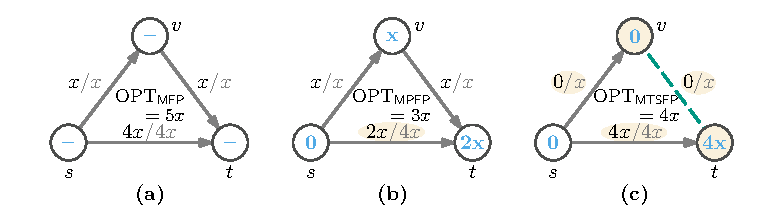
\includegraphics{switchplacement/figures/simple_switching_example_comparing_mf_mpf_mtsf.pdf}
    %
    \caption[A simple switching example that compares~\gls{mf}, 
    \gls{mpf}, and~\gls{mtsf}.]{%
    A network~\glssymbol{network} with three vertices and edges,
    capacities~\screentextcolor{KITblack50}{$\glssymbol{capacity}(\vertexa,\vertexb)$}
    \mbox{(\screentextcolor{KITblack50}{gray})}, one generator~$
    \glssymbol{generators}=\{\source\}$, one consumer~$\glssymbol{consumers} = 
    \{\sink\}$,
    susceptance~$\glssymbol{susceptance} \equiv 1$ for
    all~$(\vertexa,\vertexb)\in\glssymbol{edges}$, and voltage
    angles~\screentextcolor{THETA}{\vangle} (\screentextcolor{THETA}{blue}) for
    electrically feasible flows. The successive differences are marked
    (\hlhili{orange}). (a)~The~$\gls{mfp}(\glssymbol{network})$ is the problem
    that tries to congest all edges and has a value of~$\opt_{\gls{mfp}} = 5x$.
    (b)~The~$\gls{mpfp}(\glssymbol{network})$ with~$\opt_{\gls{mpfp}} = 3x$ is
    restricted by the path with the lowest capacity. (c)~Removing an edge with
    the lowest capacity (\screentextcolor{KITgreen}{dashed line}) helps to
    approach the~\gls{mf}. However, the value of~$\opt_{\gls{mtsfp}}$ is~$4x$. }%
    % 
    \label{ch:switching:sec:model:fig:simple_switching_example}%
\end{figure}%
%%%%%%%%%%%%%%%%%%%%%%%%%%%%%%%%%%%%%%%%%%%%%%%%%%%%%%%%%%%%%%%%%%%%%%%%%%%%%%%%
%

A flow is a function~$\glssymbol{flow}\colon\glssymbol{edges}\to\reals$ that satisfies
the
%
skew-symmetry property~$\glssymbol{flow}(\vertexa,\vertexb) = -\glssymbol{flow}(\vertexb,\vertexa)$
for all~$(\vertexa,\vertexb)\in\glssymbol{edges}$. 
%
Moreover, it has to satisfy the following flow conservation 
property~(\cref{ch:switching:sec:model:eq:flow_conservation,ch:switching:sec:model:eq:unlimited_demand_constraint,ch:switching:sec:model:eq:unlimited_generation_constraints}).
% 
For a vertex~$\vertexa\in\glssymbol{vertices}$ the~\emph{net flow} is denoted
by~$\glssymbol{netflow}(\vertexa) \coloneqq
\sum_{\{\vertexa,\vertexb\}\in\glssymbol{undirectededges}}\glssymbol{flow} 
(\vertexa,\vertexb)$.
%
Similar to~\acrlong{kcl} (\gls{kcl},
see~\cref{ch:switching:sec:model:eq:flow_conservation}) the conservation of flow
describes the flow at each vertex including the consumption or outflow to other
network layers, which is bounded by~$\realpowerdemandmin\geq 0$ and often
denoted as
demand~(\cref{ch:switching:sec:model:eq:unlimited_demand_constraint}), and
the generation limits
(\cref{ch:switching:sec:model:eq:unlimited_generation_constraints}).
%
% %%%%%%%%%%%%%%%%%%%%%%%%%%%%%%%%%%% EQUATIONS %%%%%%%%%%%%%%%%%%%%%%%%%%%%%%%%%%
\begin{align}%
\glssymbol{netflow}(\vertexa) &= 0 & \forall\vertexa\in
\glssymbol{vertices}\setminus
(\glssymbol{generators}\cup\glssymbol{consumers}),
\label{ch:switching:sec:model:eq:flow_conservation}\\%
%
-\infty\leq\glssymbol{netflow}(\vertexa) &\leq-\realpowerdemandmin(\vertexa) &
\forall\vertexa\in\glssymbol{consumers} ,
\label{ch:switching:sec:model:eq:unlimited_demand_constraint}\\%
%
0\leq\glssymbol{netflow}(\vertexa) &\leq \infty &
\forall\vertexa\in\glssymbol{generators}.%
\label{ch:switching:sec:model:eq:unlimited_generation_constraints}%
\end{align}%
%
A flow~\glssymbol{flow} is~\emph{feasible} if it obeys the thermal limits given
by the capacity constraints
(\cref{ch:switching:sec:model:eq:capacity_constraints}).

\begin{equation}%
  \fmagnitude{\glssymbol{flow}(\vertexa,\vertexb)}\leq\glssymbol{capacity}
  (\vertexa,\vertexb)
  \qquad\forall(\vertexa,\vertexb)\in\glssymbol{edges}.
  % 
  \label{ch:switching:sec:model:eq:capacity_constraints}%
\end{equation}%
% 
The~\emph{flow value}~$\glssymbol{flowvalue}(\glssymbol{network},\glssymbol{flow})$ of a
flow~\glssymbol{flow} on~\glssymbol{network} is defined
by~$\sum_{\vertexa\in\glssymbol{generators}}\glssymbol{netflow}(\vertexa)$. A
feasible flow~\glssymbol{flow} on~\glssymbol{network}
maximizing~$\glssymbol{flowvalue}(\glssymbol{network},\glssymbol{flow})$ is
called a~\acrlong{mf}~(\gls{mf}) and the problem of finding such a flow is
denoted by~$\gls{mfp}(\glssymbol{network})$. Its value is denoted
by~$\opt_{\gls{mfp}}(\glssymbol{network}) \coloneqq \max_{\glssymbol{flow}}
\glssymbol{flowvalue}(\glssymbol{network},\glssymbol{flow})$
(see~\cref{ch:switching:sec:model:fig:simple_switching_example}\screen{a}).%

However, a feasible flow neglects some physical constraints of a power flow
denoted as~\acrlong{kvl} (\gls{kvl}, \cref{ch:switching:sec:model:eq:KVL_dc_approx}).
%
%%%%%%%%%%%%%%%%%%%%%%%%%%%%%%%%%%% EQUATIONS %%%%%%%%%%%%%%%%%%%%%%%%%%%%%%%%%
\begin{align}%
  \glssymbol{susceptance}(\vertexa,\vertexb)\cdot (\glssymbol{voltageangle}(\vertexa) - \glssymbol{voltageangle}(\vertexb) -
  \glssymbol{voltageangleshift}(\vertexa,\vertexb)) &= \glssymbol{flow}(\vertexa,\vertexb)
  &\hspace*{-2mm}\forall
  (\vertexa,\vertexb)&\in\glssymbol{edges},%
  \label{ch:switching:sec:model:eq:KVL_dc_approx}%
  \\
  %
  \vanglemin(\vertexa) 
  \leq \hspace*{1.4mm}\glssymbol{voltageangle}(\vertexa)\hspace*{1.3mm} &
  \leq \vanglemax(\vertexa)&\forall\vertexa&\in\glssymbol{vertices},%
  \label{ch:switching:sec:model:eq:theta_bound}%
\end{align}%
% 
where the voltage angle is a
function~$\glssymbol{voltageangle}\colon\glssymbol{vertices}\to\reals$
describing the potential at each vertex. In general, absolute voltage angles are
used, \ie, the angle of one vertex---often the slack---is set to zero and the
others are determined from it~\cite[see][p. 40]{bollobas1998modern}. A deeper
discussion of the latter is available
in~\cref{ch:network-analyzes:sec:mathematical-model}. The voltage
angle~$\glssymbol{voltageangle}(\vertexa)$ of a
vertex~$\vertexa\in\glssymbol{vertices}$ is often limited
to~$\fmagnitude{\glssymbol{voltageangle}(\vertexa)}\leq 0.6$~radians
(see~\cref{ch:switching:sec:model:eq:theta_bound}) to improve the running
time~\parencite{Fis08,6345550}, but this may result in non-optimal solutions or
no solution at all. Note that the voltage angle differences are already covered
by the capacity
constraint~(\cref{ch:switching:sec:model:eq:capacity_constraints}) and thus, the
constraint is not mentioned here. In addition, in most~\gls{ieee} examples and
related works~$\glssymbol{voltageangleshift}\equiv 0$ representing the
transformer (phase shifter) final angle. The latter means that we assume to have
neither~\gls{facts} nor phase shift transformers on the lines. Thus, we neglect
them in the following.
% 
%%%%%%%%%%%%%%%%%%%%%%%%%%%%%%%%%%%%% FIGURE %%%%%%%%%%%%%%%%%%%%%%%%%%%%%%%%%%%
\begin{figure}[t!]%
    \centering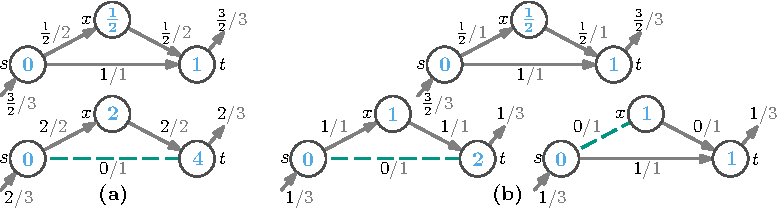
\includegraphics{switchplacement/figures/not_benefitial_simple_switching_example.pdf}
    %
    \caption[The Braess's Paradox highly depends on the network's parameters.]{%
    The Braess's Paradox highly depends on the network's parameter. A general
    observation on that was already given by~\textcite{Pas97}. This example
    network consists of three vertices, three edges, one generator, one load,
    susceptances~$\glssymbol{susceptance} \equiv 1$, and different capacity~$
    \textcolor{CAPACITY}{\glssymbol{capacity}(\edge)}$ settings
    (\textcolor{CAPACITY}{gray}) for all~$\edge\in\glssymbol{edges}$. (a) The
    capacities are chosen in such a way that switching is beneficial in that
    particular network~\glssymbol{network}. The~\gls{mpfp} has a value
    of~$\opt_{\gls{mpfp}}(\glssymbol{network}) = \nicefrac{3}{2}$, whereas
    the~\gls{mtsfp} has a value of~$\opt_{\gls{mtsfp}}(
    \glssymbol{network}) = 2$. (b) The capacities of the edges~$(\source,x)$
    and~$ (x,\sink)$ are set to~$1$. This small reconfiguration makes switching
    not beneficial anymore, since the~\gls{mpfp} has a value
    of~$\opt_{\gls{mpfp}} = \nicefrac{3}{2}
    =
    \opt_{\gls{mtsfp}}$ and any switching has a value of~$1$. }%
    %
    \label{ch:switching:sec:model:fig:when_switching_is_not_benefitial}%
\end{figure}%
%%%%%%%%%%%%%%%%%%%%%%%%%%%%%%%%%%%%%%%%%%%%%%%%%%%%%%%%%%%%%%%%%%%%%%%%%%%%%%%%
%

We call a feasible flow complying
with~\cref{ch:switching:sec:model:eq:KVL_dc_approx,ch:switching:sec:model:eq:theta_bound}
a \emph{feasible electrical flow}. A feasible electrical 
flow~\glssymbol{flow} on~\glssymbol{network}
% 
%
that maximizes~$\glssymbol{flowvalue}(\glssymbol{network},\glssymbol{flow})$ 
%
is called a maximum power flow~($\gls{mpf}$). The
corresponding problem is called the~\acrlong{mpfp}~(\gls{mpfp}) and is denoted
by~$\gls{mpfp}(\glssymbol{network})$.
%
%
The value of~$\gls{mpfp}(\glssymbol{network})$ is denoted
by~$\opt_{\gls{mpfp}}(\glssymbol{network})$ and is defined
by~$\max_{\glssymbol{flow}}\glssymbol{flowvalue}(\glssymbol{network},
\glssymbol{flow})$
(see~\cref{ch:switching:sec:model:fig:simple_switching_example}\screen{b}).
% 

For a subset~$\glssymbol{switched}\subseteq\glssymbol{undirectededges}$ we
consider the graph~$\glssymbol{graph}-\glssymbol{switched}$ and the
corresponding network~$\glssymbol{network}-\glssymbol{switched}$ where the
functions~\glssymbol{capacity} and~\glssymbol{susceptance} are restricted
to~$\glssymbol{edges}\setminus\glssymbol{switched}$.
%
We call~\glssymbol{switched} the set of switched edges (\ie, the switch is in
OFF-state for these edges). Typically not all possible switchings are feasible.
Feasibility in this context means that there is an electrically feasible flow
in~$\glssymbol{network}-\glssymbol{switched}$.
%
%
The problem of maximizing the flow value in~\glssymbol{network} while allowing
edges to be switched is called~\acrlong{mtsfp}~(\gls{mtsfp}) and its value is
denoted by~$\opt_{\gls{mtsfp}}(\glssymbol{network})
\coloneqq
% 
\max_{\glssymbol{switched}\subseteq\glssymbol{undirectededges}}
\opt_{\gls{mpfp}}(\glssymbol{network}-\glssymbol{switched})$ (see~\cref{ch:switching:sec:model:fig:simple_switching_example}\screen{c}). Such a flow
% 
obeys~\cref{ch:switching:sec:model:eq:flow_conservation,ch:switching:sec:model:eq:unlimited_demand_constraint,ch:switching:sec:model:eq:unlimited_generation_constraints,ch:switching:sec:model:eq:capacity_constraints_switching,ch:switching:sec:model:eq:linearized_switching_geq,ch:switching:sec:model:eq:linearized_switching_leq}. 
% 
Note that switching is not always beneficial as shown in~\cref{ch:switching:sec:model:fig:when_switching_is_not_benefitial}\screen{b}.
%
\begingroup
    %%%%%%%%%%%%%%%%%%%%%%%%%%%%%%%%%%% Problem %%%%%%%%%%%%%%%%%%%%%%%%%%%%%%%%%%%%
\begin{problem}[framed]{\acrlong{mtsfp}~$\gls{mtsfp}(\glssymbol{network})$}%
    Instance: & A network~\glssymbol{network}.\\
    % 
    Objective: & Find a
    set~$\glssymbol{switched}\subseteq\glssymbol{undirectededges}$ of switched
    edges such
    that~$\opt_{\gls{mpfp}}(\glssymbol{network}-\glssymbol{switched})$ is maximum
    among all choices of switched edges~\glssymbol{switched}.
\end{problem}%
    \label{ch:switching:problems:MTSF-Optimization_problem}
\endgroup
%
To model switching an edge we introduce a
function~$\glssymbol{switch}\colon\glssymbol{edges}\to\{0,1\}$, which is~$0$ if
an edge is switched and~$1$ otherwise.
%
To enforce the switching, the flow must be zero on the switched edges. We
therefore replace~\cref{ch:switching:sec:model:eq:capacity_constraints} with
\cref{ch:switching:sec:model:eq:capacity_constraints_switching}. This change is
not yet sufficient, since the KVL
(\cref{ch:switching:sec:model:eq:KVL_dc_approx}) shall only apply to the
non-switched edges. Hence, we modify this equation 
to~\cref{ch:switching:sec:model:eq:KVL_quadratic_switching}.%
%
%%%%%%%%%%%%%%%%%%%%%%%%%%%%%%%%%%% EQUATION %%%%%%%%%%%%%%%%%%%%%%%%%%%%%%%%%%
\begin{align}%
    \hspace*{-2.5mm}b(\vertexa,\vertexb)\!\cdot\! \switch(\vertexa,\vertexb)\cdot 
    (\glssymbol{voltageangle}
    (\vertexa) - \glssymbol{voltageangle}(\vertexb))
    &= \glssymbol{flow}(\vertexa,\vertexb) &\forall 
    (\vertexa,\vertexb)\in\glssymbol{edges},\hspace*{-1mm}
    \label{ch:switching:sec:model:eq:KVL_quadratic_switching}\\%
    %
    \fmagnitude{\glssymbol{flow}(\vertexa,\vertexb)}&\leq 
    \glssymbol{switch}(\vertexa,\vertexb)\cdot
    \glssymbol{capacity}(\vertexa,\vertexb)
    \hspace*{-1mm} &
    \forall(\vertexa,\vertexb)\in\glssymbol{edges}.\hspace*{-1mm}
    % 
    \label{ch:switching:sec:model:eq:capacity_constraints_switching}%
\end{align}%
%
\cref{ch:switching:sec:model:eq:KVL_quadratic_switching} can be linearized by
either adding two big-$M$ constraints
(\cref{ch:switching:sec:model:eq:linearized_switching_geq,ch:switching:sec:model:eq:linearized_switching_leq})
or one indicator constraints
(\cref{ch:switching:sec:model:eq:indicator_constraint}), where~$M$ is a suitably
large constant.
%
\begin{align}%
  \hspace*{-3mm}\glssymbol{susceptance}(\vertexa,\vertexb)\cdot
  (\glssymbol{voltageangle}(\vertexa) - \glssymbol{voltageangle}(\vertexb)) &+
  (1 - \glssymbol{switch}(\vertexa,\vertexb) ) M\geq
  \glssymbol{flow}(\vertexa,\vertexb)\hspace*{-2mm} &\forall
  (\vertexa,\vertexb)\in\glssymbol{edges},\hspace*{-1mm}
  \label{ch:switching:sec:model:eq:linearized_switching_geq}\\%
  %
  \hspace*{-3mm}\glssymbol{susceptance}(\vertexa,\vertexb)\cdot (
  \glssymbol{voltageangle}(\vertexa) - \glssymbol{voltageangle}(\vertexb)) &-
  (1 - \glssymbol{switch}(\vertexa,\vertexb) ) M\leq \glssymbol{flow}(\vertexa,\vertexb)\hspace*{-2mm} &\forall 
  (\vertexa,\vertexb)\in\glssymbol{edges},\hspace*{-1mm}
  \label{ch:switching:sec:model:eq:linearized_switching_leq}\\%
  % 
  \hspace*{-1mm}\glssymbol{switch}(\vertexa,\vertexb) = 1 \Rightarrow \glssymbol{susceptance}
  (\vertexa,\vertexb)\cdot(
  \glssymbol{voltageangle}(\vertexb) - \glssymbol{voltageangle}(\vertexa) )
  &\hphantom{- (1 - \glssymbol{switch}(\vertexa,\vertexb) ) M .} =
  \glssymbol{flow}(\vertexa,\vertexb) &\forall
  (\vertexa,\vertexb)\in\glssymbol{edges}.\hspace*{-1mm}
  \label{ch:switching:sec:model:eq:indicator_constraint}
  % 
\end{align}%
%
The parameter~$M$ must be reasonably large to not impose any implicit voltage
angle difference limit at the edge~$(\vertexa,\vertexb)\in\glssymbol{edges}$. In
general, one can choose~$M$ for each
edge~$(\vertexa,\vertexb)\in\glssymbol{edges}$ by~$M{(\vertexa,\vertexb)}$ equal
to~$\max\left\{\sum_{\edge\in\pi(\vertexa,\vertexb)}\glssymbol{susceptance}(\edge)^{-1}
\glssymbol{capacity} (\edge)\right\}$,
%
%
where the maximum ranges over all simple paths~$\fpath{}{\vertexa}{\vertexb}$
from~\vertexa to~\vertexb. It then suffices to set $M
=\max_{(\vertexa,\vertexb)\in\glssymbol{edges}}M{(\vertexa,\vertexb)}$~
\parencite{Bin01a}. However, it is \NP-hard to calculate the longest path
\parencite{Karger1997}. It is simpler to set~$M(\vertexa,\vertexb) =
\glssymbol{susceptance}(\vertexa,\vertexb) \cdot $
$\sum_{\edge\in\glssymbol{edges}}
\nicefrac{\glssymbol{capacity}(\edge)}
{\glssymbol{susceptance}(\edge)}$. If we restrict the voltage
angle~\glssymbol{voltageangle} to~$0.6$ radians
in~\cref{ch:switching:sec:model:eq:theta_bound}, which is
common~\parencite{6345550,5401077}, we can use~$M{(\vertexa,\vertexb)} =
1.2\cdot\fmagnitude{\glssymbol{susceptance}(\vertexa,\vertexb)}$. Note that this
decreases the solution space and possibly removes feasible and optimal
solutions. Thus, this restriction can improve the running time, but might lead
to other results and is thus debatable, from a physical point of view.
% 
In general, we have lower and upper bounds for
generators~$
\realpowergenerationmin,
\realpowergenerationmax
\colon
\glssymbol{generators}
\to
\posreals
\cup\{\infty\}$,
and demands~$
\realpowerdemandmin,
\realpowerdemandmax
\colon
\glssymbol{consumers}
\to
\posreals
\cup
\{\infty\}$ for~$\vertexa\in\glssymbol{consumers}$ such
that~\cref{ch:switching:sec:model:eq:unlimited_demand_constraint,ch:switching:sec:model:eq:unlimited_generation_constraints}
become~\cref{ch:switching:sec:model:eq:demand_constraint,ch:switching:sec:model:eq:generation_constraints},
respectively, and the network is defined by~$\dcnetworktuple$. A network with
these additional bounds is called~\emph{bounded}.
%
% %%%%%%%%%%%%%%%%%%%%%%%%%%%%%%%%%%% EQUATIONS %%%%%%%%%%%%%%%%%%%%%%%%%%%%%%%%%%
\begin{align}%
  -\realpowerdemandmax(\vertexa)\leq\glssymbol{netflow}(\vertexa) &\leq 
  -\realpowerdemandmin(\vertexa) & \forall\vertexa\in\glssymbol{consumers}
  \label{ch:switching:sec:model:eq:demand_constraint}\\%
  %
  \realpowergenerationmin(\vertexa)\leq\glssymbol{netflow}(\vertexa) &\leq 
  \realpowergenerationmax(\vertexa) & \forall\vertexa\in\glssymbol{generators}
  \label{ch:switching:sec:model:eq:generation_constraints}%
\end{align}%
%
A~$\gls{mtsf}$ obeying the latter constraints is a \emph{bounded~\gls{mtsf}}.
Note that fixing the demands~$\realpowerdemandmin (\vertexa) =
\realpowerdemandmax(\vertexa) = \realpowerdemand(\vertexa)$ and
generations~$\realpowergenerationmin(\vertexa) = \realpowergenerationmax
(\vertexa) = \realpowergeneration(\vertexa)$ leads to
a~\acrlong{dc}~\acrlong{feas} (\gls{dc}~\gls{feas}) also known as~\acrlong{pf}
(\gls{pf}) that is the search for a feasible electrical flow by given demands
and generations. We discussed the latter problem in more detail
in~\cref{ch:network-analysis}.

Suppose every generator~$\vertexa\in\glssymbol{generators}$ has its own
generation cost function~$\gamma_\vertexa\colon\reals\to\posreals$ representing
the cost for generating the power~$\glssymbol{netflow}(\vertexa)$.
%
The problem of minimizing the generation costs of all
generators~$\vertexa\in\glssymbol{generators}$ while maintaining a 
feasible electrical flow in a bounded network with $\realpowerdemandmin(\vertexa) = 
\realpowerdemandmax(\vertexa) = \realpowerdemand(\vertexa)$ (\ie,
% 
\cref{ch:switching:sec:model:eq:flow_conservation,ch:switching:sec:model:eq:capacity_constraints,ch:switching:sec:model:eq:capacity_constraints,ch:switching:sec:model:eq:KVL_dc_approx,ch:switching:sec:model:eq:theta_bound,ch:switching:sec:model:eq:demand_constraint,ch:switching:sec:model:eq:generation_constraints})
% 
is called~\acrlong{opfp}~$\gls{opfp}(\glssymbol{network})$. The
value of~$\gls{opfp}(\glssymbol{network})$ is denoted by~$\opt_{\gls{opfp}}(
\glssymbol{network}) = \min \sum_{\vertexa\in\glssymbol{generators}}
\fcost{\vertexa}(\glssymbol{netflow}(\vertexa))$. The problem of finding
a flow with value~$\opt_{\gls{opfp}}(\glssymbol{network})$
by allowing edges to be switched (\ie,
% 
\cref{ch:switching:sec:model:eq:flow_conservation,ch:switching:sec:model:eq:theta_bound,ch:switching:sec:model:eq:capacity_constraints_switching,ch:switching:sec:model:eq:linearized_switching_geq,ch:switching:sec:model:eq:linearized_switching_geq,ch:switching:sec:model:eq:demand_constraint,ch:switching:sec:model:eq:generation_constraints})
% 
is called~\acrlong{otsp}~$\gls{otsp}(\glssymbol{network})$ with 
value~$\opt_{\gls{otsp}}(\glssymbol{network})=
\min_{\glssymbol{switched}\subseteq\glssymbol{undirectededges}}\opt_{
\gls{opfp}}(
\glssymbol{network}\!-\!
\glssymbol{switched})$ with~$\glssymbol{switched}$ being the set of switched
edges.
% 
\begingroup
    %
%%%%%%%%%%%%%%%%%%%%%%%%%%%%%%%%%%% Problem %%%%%%%%%%%%%%%%%%%%%%%%%%%%%%%%%%%%
\begin{problem}[framed]{\acrlong{otsp}~$\gls{otsp}(\glssymbol{network})$}%
  % 
  Instance: & A network~\glssymbol{network}.\\%
  % 
  Objective: & Find a set~$\glssymbol{switched}\subseteq\glssymbol{edges}$ and
  an electrically feasible flow~\glssymbol{flow} in~$
  \glssymbol{network}-\glssymbol{switched}$ such that the sum of the generation
  costs~$\sum_{\vertexa\in\glssymbol{generators}}\gamma_\vertexa\left(
  \glssymbol{netflow}(\vertexa)\right)$ is minimized.%
  %
\end{problem}%
    \label{ch:switching:problems:OTS-Optimization_problem}
\endgroup
%
Note that neither the~\gls{mtsfp} nor the~\gls{otsp} minimize the number of
switches. This would result in a~$\min$-$\max$-problem  that is harder to solve
than the presented basic variants
(see~\cref{ch:switching:sec:problem-definition} on
Page~\pageref{ch:switching:sec:problem-definition}). From~\textcite[Lemma
4]{Leh15a} it further follows that the~\gls{mtsfp} and
the~\acrlong{mffp}~(\gls{mffp}) are polynomial-time solvable on trees. Thus, for
trees we get the following relationship.
% 
$$\opt_{\gls{mpfp}}(\glssymbol{network}) 
= \opt_{\gls{mtsfp}}(\glssymbol{network})
= \opt_{\gls{mffp}}(\glssymbol{network})
= \opt_{\gls{mfp}}(\glssymbol{network}).
% 
\label{ch:switching:structure:tree}
$$
% 
If it is clear, which network is being referred to, we may omit the explicit
reference~\glssymbol{network} and write~$\glssymbol{problems}$
and~$\opt_{\glssymbol{problems}}$ instead
of~$\glssymbol{problems}(\glssymbol{network})$
and~$\opt_{\glssymbol{problems}}(\glssymbol{network})$,
where~$\glssymbol{problems}$ is a particular problem~(\eg,
\gls{mtsfp}). The common constraints of~\gls{mtsfp} and~\gls{otsp} are the base
constraints for
the~\acrlong{rop}~(\gls{rop})~\parencite{van2011vehicle,COFFRIN2015144}
and~\gls{tnep}~\parencite{Hem13}.
% 
%%%%%%%%%%%%%%%%%%%%%%%%%%%%%%%%%%%%%%%%%%%%%%%%%%%%%%%%%%%%%%%%%%%%%%%%%%%%%%%
\begin{landscape}
    \begin{table}
        % 
        % latex table generated in R 3.2.2 by xtable 1.8-0 package
% Wed Jan 27 11:17:04 2016
% \vspace{-1.5cm}
{\setlength{\tabcolsep}{0.3em}}
{\renewcommand{\arraystretch}{1}}% for the vertical padding
% \footnotesize
\begin{tabular}{
  l>{\centering\arraybackslash}%
  m{1.5cm}>{\centering\arraybackslash}%
  m{3.0cm}>{\centering\arraybackslash}%
  m{1.7cm}cccc>{\centering\arraybackslash}%
  m{2.7cm}>{\centering\arraybackslash}%
  m{2.7cm}>{\centering\arraybackslash}%
  m{1.1cm}cc%
}%
\toprule
  & 
  & \multicolumn{6}{c}{\textbf{Network Properties}}
  & \multicolumn{2}{c}{\textbf{Complexity} }
  & \multicolumn{3}{c}{\textbf{Algorithms}}
  \\
%-------------------------------------------------------------------------------
%-------------------------------------------------------------------------------
 \cmidrule(lr){3-8}\cmidrule(lr){9-10}\cmidrule(lr){11-13}
  & \multirow[c]{-2}*{\textbf{Problem}}
  & \multicolumn{1}{c}{Graph Structure}
  & \multicolumn{1}{c}{Example}
  & \screentextcolor{GENERATOR}{$\fmagnitude{\glssymbol{generators}}$} 
  & \screentextcolor{CONSUMER}{$\fmagnitude{\glssymbol{consumers}}$}
  & \screentextcolor{SUSCEPTANCE}{$\glssymbol{susceptance}$}
  & \screentextcolor{CAPACITY}{$\glssymbol{capacity}$}
  & \multicolumn{1}{c}{Hardness}
  & \multicolumn{1}{c}{Reference}
  & \multicolumn{1}{c}{Name} 
  & \multicolumn{1}{c}{\screentextcolor{SUSCEPTANCE}{$\glssymbol{susceptance}$}}
  & \multicolumn{1}{c}{\screentextcolor{CAPACITY}{$\glssymbol{capacity}$}}
  \\
%-------------------------------------------------------------------------------
%-------------------------------------------------------------------------------
 \midrule\addlinespace
%-------------------------------------------------------------------------------
%-------------------------------------------------------------------------------
\rowcolor{Table-Line-Marker}
%-------------------------------------------------------------------------------
1\label{ch:switching:sec:exploit_structural_characteristics:tbl:tree}
& \gls{mtsfp} and~\gls{otsp}
& tree graphs
& \raisebox{-0.5cm}[0pt][0pt]{
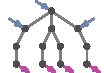
\includegraphics{switchplacement/figures/graph_structure-tree.pdf}%
}
& \screentextcolor{GENERATOR}{$\infty$}
& \screentextcolor{CONSUMER}{$\infty$}
& \screentextcolor{SUSCEPTANCE}{--}
& \screentextcolor{CAPACITY}{--}
& polynomial-time solvable
& 
\cref{ch:network-analyzes:sec:mathematical-model:lem:pf-matrix-is-tum}, 
\cref{ch:facts:thm:fvs},
\cref{ch:foundations:sec:graph-theoretical-flows} p.\ 
\pageref{ch:foundations:sec:graph-theoretical-flows:para:maximum-flow-problem}
& \gls{mf} & \screentextcolor{SUSCEPTANCE}{$\infty$} &
\screentextcolor{CAPACITY}{$\infty$}
\\\addlinespace\addlinespace
% 
2\label{ch:switching:sec:exploit_structural_characteristics:tbl:penrose_minor}
& \gls{mtsfp} and~\gls{otsp}
& penrose-minor-free graphs
& \raisebox{-0.5cm}[0pt][0pt]{
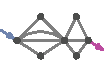
\includegraphics{switchplacement/figures/graph_structure-penrose_minor_free_graph.pdf}}
& \screentextcolor{GENERATOR}{1}
& \screentextcolor{CONSUMER}{1}
& \screentextcolor{SUSCEPTANCE}{--}
& \screentextcolor{CAPACITY}{--}
& polynomial-time solvable
& \cref{ch:switching:sec:exploit_structural_characteristics,ch:switching:sec:computing_one_dtp}
& \gls{dtp}
& \screentextcolor{SUSCEPTANCE}{$\infty$}
& \screentextcolor{CAPACITY}{$\infty$}
\\\addlinespace\addlinespace
% 
\rowcolor{Table-Line-Marker}
%-------------------------------------------------------------------------------
& \gls{mtsfp}
& series-parallel
& % --
& % --
& % --
& \screentextcolor{SUSCEPTANCE}{$\infty$}
& \screentextcolor{CAPACITY}{$\infty$}
& % --
& \parencite{Koc16}
& % --
& % --
& % --
\\
% 
\rowcolor{Table-Line-Marker}
%-------------------------------------------------------------------------------
\multirow{-2}*{3}
\label{ch:switching:sec:exploit_structural_characteristics:tbl:series_parallel}
& and~\gls{otsp}% \acrshort{mtsf} and~\acrshort{ots}
& graphs % series-parallel graphs
& \multirow{-2}*{\raisebox{-0.5cm}[0pt][0pt]{%{-\totalheight}
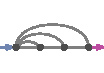
\includegraphics{switchplacement/figures/graph_structure-series_parallel_graph.pdf}}}
& \multirow{-2}*{\screentextcolor{GENERATOR}{1}}
& \multirow{-2}*{\screentextcolor{CONSUMER}{1}}
& \cellcolor{KITpalegreen15}\screentextcolor{SUSCEPTANCE}{$\infty$}
& \cellcolor{KITpalegreen15}\screentextcolor{CAPACITY}{$1$}
& \multirow{-2}*{\NP-hard}
& \cellcolor{KITpalegreen15}\cref{ch:switching:sec:complexity}
& \multirow{-2}*{--}
& \multirow{-2}*{\screentextcolor{SUSCEPTANCE}{--}} 
& \multirow{-2}*{\screentextcolor{CAPACITY}{--}}
\\\addlinespace\addlinespace
% 
4\label{ch:switching:sec:exploit_structural_characteristics:tbl:cactus}
& \gls{mtsfp} and~\gls{otsp}
& cacti with maximum degree of~$3$
& \raisebox{-0.5cm}[0pt][0pt]{%{-\totalheight}
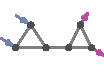
\includegraphics{switchplacement/figures/graph_structure-cacti_graph.pdf}}
& \screentextcolor{GENERATOR}{$\infty$}
& \screentextcolor{CONSUMER}{$\infty$}
& \screentextcolor{SUSCEPTANCE}{1}
& \screentextcolor{CAPACITY}{$\infty$}
& \NP-hard
& \parencite{Leh14}
& \gls{maxst} (see~\cref{ch:switching:sec:approximation_algorithm_on_cacti})
& \screentextcolor{SUSCEPTANCE}{--}
& \screentextcolor{CAPACITY}{--}
\\\addlinespace\addlinespace
% 
\rowcolor{Table-Line-Marker}
%-------------------------------------------------------------------------------
5\label{ch:switching:sec:exploit_structural_characteristics:tbl:2_level_tree}
& \gls{mtsfp} and~\gls{otsp}
& 2-level trees
& \raisebox{-0.5cm}[0pt][0pt]{%{-\totalheight}
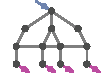
\includegraphics{switchplacement/figures/graph_structure-two_level_tree.pdf}}
& \screentextcolor{GENERATOR}{1}
& \screentextcolor{CONSUMER}{$\infty$}
& \screentextcolor{SUSCEPTANCE}{$\infty$}
& \screentextcolor{CAPACITY}{$\infty$}
& \NP-hard
& \parencite{Leh14}
& --
& \screentextcolor{SUSCEPTANCE}{--}
& \screentextcolor{CAPACITY}{--}
\\\addlinespace\addlinespace
% 
6\label{ch:switching:sec:exploit_structural_characteristics:tbl:plane_graph}
& \gls{mtsfp} and~\gls{otsp}
& planar graph with~$\max$ degree of~$3$
& \raisebox{-0.5cm}[0pt][0pt]{%{-\totalheight}
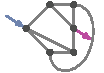
\includegraphics{switchplacement/figures/graph_structure-plane_graph.pdf}}
& \screentextcolor{GENERATOR}{1}
& \screentextcolor{CONSUMER}{1}
& \screentextcolor{SUSCEPTANCE}{$\infty$}
& \screentextcolor{CAPACITY}{1}
& strongly~\NP-hard
& \parencite{Leh14}
& --
& \screentextcolor{SUSCEPTANCE}{--}
& \screentextcolor{CAPACITY}{--}
\\\addlinespace\addlinespace
% 
\rowcolor{Table-Line-Marker}
%-------------------------------------------------------------------------------
& \gls{mtsfp}
& % --
& % --
& \screentextcolor{GENERATOR}{2}
& \screentextcolor{CONSUMER}{2}
& % --
& % --
& % --
& \parencite{Leh14}
& % --
& % --
& % --
\\
% 
\rowcolor{Table-Line-Marker}
%-------------------------------------------------------------------------------
\multirow{-2}*{7}
\label{ch:switching:sec:exploit_structural_characteristics:tbl:arbitrary_graph}
& \cellcolor{KITpalegreen15}\gls{otsp} 
& \multirow{-2}*{arbitrary graphs}
& \multirow{-2}*{\raisebox{-0.5cm}[0pt][0pt]{%{-\totalheight}
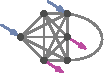
\includegraphics{switchplacement/figures/graph_structure-arbitrary_graph.pdf}}}
& \cellcolor{KITpalegreen15}\screentextcolor{GENERATOR}{1}
& \cellcolor{KITpalegreen15}\screentextcolor{CONSUMER}{$\infty$}
& \multirow{-2}*{\screentextcolor{SUSCEPTANCE}{$\infty$}}
& \multirow{-2}*{\screentextcolor{CAPACITY}{$\infty$}}
& \multirow{-2}*{non-\APX}
& \cellcolor{KITpalegreen15}\parencite{Leh14}
& \multirow{-2}*{--}
& \multirow{-2}*{\screentextcolor{SUSCEPTANCE}{--}} 
& \multirow{-2}*{\screentextcolor{CAPACITY}{--}}
\\\addlinespace\addlinespace
% 
%-------------------------------------------------------------------------------
%-------------------------------------------------------------------------------
   \bottomrule
\end{tabular}

        % 
        \vspace*{-2.0cm}
        % 
        \caption[Overview of results on the complexity of switching.]{Overview
        of known results on the complexity of the~\gls{mtsfp} and~\gls{otsp}.
        The complexity increases from top to bottom as shown in the hardness
        column. Note that the major aspects that influence the complexity of the
        problem are the graph structure of~\glssymbol{graph}, the number of
        \screentextcolor{GENERATOR} {generators~\glssymbol{generators}}, the
        number of
        \screentextcolor{CONSUMER}{consumers~\glssymbol{consumers}}, the
        \screentextcolor{SUSCEPTANCE}{susceptance~\glssymbol{susceptance}}, and the
        \screentextcolor{CAPACITY}{capacity~$\glssymbol{capacity}$}. If there
        are multiple results or if the results differ for~\gls{mtsfp}
        and~\gls{otsp}, we colored the relating entries
        in~\myhl{KITpalegreen15}{green}.}
        % 
        \label{ch:switching:sec:complexity:tbl:complexity-overview}
        % 
    \end{table}
\end{landscape}
% 
%%%%%%%%%%%%%%%%%%%%%%%%%%%%%%%%%%%%%%%%%%%%%%%%%%%%%%%%%%%%%%%%%%%%%%%%%%%%%%%%
\section{Complexity Considerations of using Discrete Control Units}
\label{ch:switching:sec:complexity}
%%%%%%%%%%%%%%%%%%%%%%%%%%%%%%%%%%%%%%%%%%%%%%%%%%%%%%%%%%%%%%%%%%%%%%%%%%%%%%%%
% 
In~\cref{ch:switching:sec:model}, we showed that switching introduces a
quadratic constraint
(see~\cref{ch:switching:sec:model:eq:KVL_quadratic_switching}). Note that models
with quadratic constraints and linear objectives are in
general~\NP-hard~\parencite[278]{Sah74}. The proof uses a reduction from
the~\acrlong{ssp} (\gls{ssp}; see~\textcite[p.245; MP2]{Gar79}
and~\textcite[p.447; MP5]{Aus99} for more information).
% 
However, the quadratic constraint can be replace by a big-M constraint
(see~\cref{ch:switching:sec:model:eq:linearized_switching_geq,ch:switching:sec:model:eq:linearized_switching_leq})
or an indicator constraint
(see~\cref{ch:switching:sec:model:eq:indicator_constraint}). Thus, we lose the
bilinearity and the constraint becomes linear.
% 
%%%%%%%%%%%%%%%%%%%%%%%%%%%%%%%%%%%%%%%%%%%%%%%%%%%%%%%%%%%%%%%%%%%%%%%%%%%%%%%%
\paragraph{Problem Definitions}
\label{ch:switching:sec:problem-definition}
%%%%%%%%%%%%%%%%%%%%%%%%%%%%%%%%%%%%%%%%%%%%%%%%%%%%%%%%%%%%%%%%%%%%%%%%%%%%%%%%
% 
In~\cref{ch:switching:sec:model}, we already defined the optimization
problems~\gls{mtsfp} and~\gls{otsp}. However, in this section we give a finer
granularity of the problem definitions concerning switching to increase the
understanding of the different problems that can be tackled.
% 
The first problem considers switching with a fixed number of preinstalled
switches---meaning~$\gls{switched}\subseteq
\gls{undirectededges}$ is already given---and is
called~$\gls{mtsfp}(\glssymbol{network},\glssymbol{switched})$ and its
value is defined by~$
\opt_{\gls{mtsfp}}(\glssymbol{network},\glssymbol{switched}) \coloneqq
\max_{\{\glssymbol{switch}(\edge)\in\{0,1\}\mid\edge\in
\glssymbol{switched}\}}\allowbreak
\opt_{\gls{mpfp}}(\glssymbol{network}-\bigcup\{\edge\mid\edge\in
\glssymbol{switched}\land\glssymbol{switch}(\edge)=0\})$. The problem is defined
in the following.
% 
\begingroup
    %%%%%%%%%%%%%%%%%%%%%%%%%%%%%%%%%%% Problem %%%%%%%%%%%%%%%%%%%%%%%%%%%%%%%%%%%%
\begin{problem}[framed]{\gls{mtsf}~Problem with Fixed Switches~$\gls{mtsfp}
(\glssymbol{network},\glssymbol{switched})$} 
    % 
    Instance: & A network~\glssymbol{network} and a
    set~$\glssymbol{switched}\subseteq\glssymbol{undirectededges}$.
    \\
    % 
    Objective: & Find a switching~$\glssymbol{switch}(\edge)\in\{0,1\}$ for
    all~$\edge\in\glssymbol{switched}$ such that~$\opt_{\gls{mpfp}}
    (\glssymbol{network}-\{\edge\mid\edge\in
    \glssymbol{switched}\land\glssymbol{switch}(\edge)=0\})$ is maximum among
    all choices of~$\glssymbol{switch}$.
    % 
\end{problem} 
%%%%%%%%%%%%%%%%%%%%%%%%%%%%%%%%%%%%%%%%%%%%%%%%%%%%%%%%%%%%%%%%%%%%%%%%%%%%%%%%
    \label{ch:switching:problems:MTSF_fixed_number_switches-optimization-problem}
\endgroup
% 
The next problem definition will be the first placement problem that relaxes the
definition in the sense that only the number of switches is fixed
by~$k\in\naturals$ with~$\fmagnitude{\glssymbol{switched}} = k$, but the
placement of the switches---meaning the
set~$\glssymbol{switched}\subseteq\glssymbol{undirectededges}$---is unknown.
Thus, we are interested in a maximum possible flow for a
network~\glssymbol{network} and a fixed number of switches~$
\fmagnitude{\glssymbol{switched}} = k$. The problem is called~$\gls{mtsfp}(
\glssymbol{network},k)$ and its value is defined by~$
% 
\opt_{\gls{mtsfp}}(\glssymbol{network},k)
\coloneqq
\max_{
  \glssymbol{switched}\subseteq\glssymbol{undirectededges}
}
\opt_{\gls{mpfp}}(\glssymbol{network}-\glssymbol{switched})
% 
$ with~$\fmagnitude{\glssymbol{switched}} = k$.%
%
\begingroup
    %%%%%%%%%%%%%%%%%%%%%%%%%%%%%%%%%%% Problem %%%%%%%%%%%%%%%%%%%%%%%%%%%%%%%%%%%%
\begin{problem}[framed]{\mtsf~Problem with~$k$-Switches~$\gls{mtsfp}(\glssymbol{network},k)$}
    % 
    Instance: & A network~\glssymbol{network} and a parameter~$k\in\naturals$.
    \\
    % 
    Objective: & Find a set~$\glssymbol{switched}\subseteq
    \glssymbol{undirectededges}$ of switches
    with~$\fmagnitude{\glssymbol{switched}} = k$ such that~$\opt_{\gls{mpfp}}
    (\glssymbol{network}-\glssymbol{switched})$ is maximum among all choices
    of~\glssymbol{switched}.
    % 
\end{problem} 
%%%%%%%%%%%%%%%%%%%%%%%%%%%%%%%%%%%%%%%%%%%%%%%%%%%%%%%%%%%%%%%%%%%%%%%%%%%%%%%%
    \label{ch:switching:problems:MTSF_with_k_switches-Optimization_problem}
\endgroup
% 
Assume that we have no limitation on the number of switches---meaning the number
of switches can be~$\fmagnitude{\glssymbol{switched}} =
\fmagnitude{\glssymbol{undirectededges}}=k$. Thus, the problem to find a maximum
power
flow in network~$\glssymbol{network}$ by allowing as many switches as possible
(\ie, some~$k\in\naturals$) is called~$
% 
  \gls{mtsfp}(\glssymbol{network})
% 
$ with value~$
% 
\opt_{\gls{mtsfp}}(\glssymbol{network})
\coloneqq
\max_{k}\opt_{\gls{mtsfp}}(\glssymbol{network},k)
% 
$.
% 
\begingroup
    %%%%%%%%%%%%%%%%%%%%%%%%%%%%%%%%%%% Problem %%%%%%%%%%%%%%%%%%%%%%%%%%%%%%%%%%%%
\begin{problem}[framed]{\acrlong{mtsfp}~$\gls{mtsfp}(\glssymbol{network})$}%
    Instance: & A network~\glssymbol{network}.\\
    % 
    Objective: & Find a
    set~$\glssymbol{switched}\subseteq\glssymbol{undirectededges}$ of switched
    edges such
    that~$\opt_{\gls{mpfp}}(\glssymbol{network}-\glssymbol{switched})$ is maximum
    among all choices of switched edges~\glssymbol{switched}.
\end{problem}%
    \label{ch:switching:problems:MTSF_with_k_switches-Optimization_problem:2}
\endgroup
% 
The latter problem allows as many switches as necessary to obtain a best
possible power flow. However, when there is only one generator and one demand
the maximum number of switches~$\fmagnitude{\glssymbol{switched}}$ is restricted
by~$\fmagnitude{\glssymbol{vertices}}-1$ that represents a tree. Removing more
edges would lead---independent on the generation limits---to an infeasible
solution, since some demands are cut-off from any generator. If we have multiple
generators and demands the maximum number would be restricted by a
forest~$\fmagnitude{\glssymbol{vertices}}-k$, where~$k$ represents the number of
connected components. Note that the number of connected components can be
still~$k=1$.

In general an desirable investigation is the minimum number of
switches---meaning the smallest~$k$---such that we get the same value
as~$\opt_{\gls{mtsfp}}(\glssymbol{network})$. This problem is called~$
% 
\opt_{\gls{mnsp}}(\glssymbol{network})
\coloneqq
\min_{
  \opt_{\gls{mtsfp}}(\glssymbol{network},k)
  =
  \opt_{\gls{mtsfp}
}(\network)} k
% 
$ with the value~$\opt_{\gls{mtsfp}}(\glssymbol{network})$. 
% 
\begingroup
    %%%%%%%%%%%%%%%%%%%%%%%%%%%%%%%%%%% Problem %%%%%%%%%%%%%%%%%%%%%%%%%%%%%%%%%%%%
\begin{problem}[framed]{\acrlong{mnsp}
    under~\gls{mtsf}~$\gls{mnsp}(\glssymbol{network},k)$} 
    % 
    Instance: & A network~\glssymbol{network} and~$k\in\naturals$.\\
    % 
    Question: & Is it possible to remove a set of edges~$
    \glssymbol{switched}\subseteq\glssymbol{edges}$
    such that $k = \fmagnitude{\glssymbol{switched}}$ is minimum among all
    choices of~$\opt_{\gls{mtsfp}}(\glssymbol{network})$?
    % 
\end{problem} 
%%%%%%%%%%%%%%%%%%%%%%%%%%%%%%%%%%%%%%%%%%%%%%%%%%%%%%%%%%%%%%%%%%%%%%%%%%%%%%%%
    \label{ch:switching:problems:MNS_under_MTSF-Optimization_problem}
\endgroup
% 
Note that similar definitions can be made for the~\gls{otsp}. An overview of the
switching related problems is given
in~\cref{app:problems:discrete-placement-problems}.
% 
\paragraph{Decision Problems}
% 
\gls{mtsfp} is an optimization problem that involves searching for the best
solution from some large set of solutions. Any optimization problem can be
transformed into a decision problem by asking whether the optimum value is at
least or at most~$k$ for some~$k\in\reals$. We denote the corresponding decision
problem for~$\gls{mtsfp}(\glssymbol{network})$ by~\kmtsfp.
%
\begingroup
    %%%%%%%%%%%%%%%%%%%%%%%%%%%%%%%%%%% Problem %%%%%%%%%%%%%%%%%%%%%%%%%%%%%%%%%%%%
\begin{problem}[framed]{\kMTSFP~\kmtsfp$(\glssymbol{network},k)$} 
    Instance: & A network~\glssymbol{network} and
    $k\in\posrationals$.\\
    % 
    Question: & Is it possible to remove a set of edges~\glssymbol{switched} such
    that there is an electrically feasible flow~\glssymbol{flow} in
    $\glssymbol{network}-\glssymbol{switched}$ with flow
    value~$\glssymbol{flowvalue}( \glssymbol{network} - 
    \glssymbol{switched}, \glssymbol{flow}) \geq k$?%
    % 
\end{problem} 
%%%%%%%%%%%%%%%%%%%%%%%%%%%%%%%%%%%%%%%%%%%%%%%%%%%%%%%%%%%%%%%%%%%%%%%%%%%%%%%%
    \label{ch:switching:problems:MNS_under_MTSF-Decision_Problem}
\endgroup
% 
Note that decision problems are often used to show that a particular problem
is~\NP-hard. We will use this problem
in~\cref{ch:switching:sec:complexity:subsec:np_hardness_Source_Sink_MTSF_capacity1}
to show that~$\gls{mtsfp}(\glssymbol{network})$ is~\NP-hard. An overview of the
switching decision problems can be found
in~\cref{app:problems:discrete-placement-problems}.
% 
%%%%%%%%%%%%%%%%%%%%%%%%%%%%%%%%%%%%%%%%%%%%%%%%%%%%%%%%%%%%%%%%%%%%%%%%%%%%%%%%
\subsection{Literature Overview}
\label{ch:switching:sec:complexity:subsec:overview}
%%%%%%%%%%%%%%%%%%%%%%%%%%%%%%%%%%%%%%%%%%%%%%%%%%%%%%%%%%%%%%%%%%%%%%%%%%%%%%%%
% 
We will see
in~\cref{ch:switching:sec:exploit_structural_characteristics:def:penrose-graph}
(see
also~\cref{ch:switching:sec:exploit_structural_characteristics:subsec:dtp_analyses,ch:switching:sec:exploit_structural_characteristics:fig:forbidden_minor})
that for single-source single-sink penrose-minor-free graphs
(see~\cref{ch:switching:sec:complexity:tbl:complexity-overview}--\screen{1})
the~$\gls{mtsfp}(\glssymbol{network})$ is poly\-no\-mi\-al-time solvable. We
will look at this structure
in~\cref{ch:switching:sec:exploit_structural_characteristics:subsec:dtp}.
However, \textcite{Koc16} showed that for arbitrary
susceptance~\glssymbol{susceptance} and capacity~$\glssymbol{capacity}$ this
problem is already~\NP-hard\footnote{We found out about that proof after the
publication of the later proof in~
\parencite{Gra18} thanks to Thomas William Brown.}.
In~\cref{ch:switching:sec:complexity:subsec:np_hardness_Source_Sink_MTSF_capacity1},
we will provide a different reduction that is also a generalization of the proof
of~\textcite{Koc16}. Contrary to series-parallel graphs, cactus graphs have the
special property that the cycles in a cactus do not share an edge. Thus, the
dependencies on the voltage angles of a vertex decrease. Though, for
single-source single-sink this problem is polynomial-time solvable, it becomes
already~\NP-hard for an arbitrary number of generators and consumers
(see~\cref{ch:switching:sec:complexity:tbl:complexity-overview}--\screen{3}).
\textcite[pp.8ff.; Section 5]{Leh14} motivated another non-standard graph
structure from the disaster management. The idea is that after a blackout
a~\gls{tso} will try to recover the power grid by establishing a tree-like
structure. The graph structure is denoted by N-level tree
(see~\cref{ch:switching:sec:complexity:tbl:complexity-overview}--\screen{4}),
which has a generator at the root and consumers at the leaves. For each level
there is a total order of the vertices that also defines the intra-level
neighbors of a vertex. The tree allows intra-level connections to direct
neighbors. Note that these intra-level connections cause cycles that share edges
with other cycles. Thus, this structure is more complex than a cactus. The next
graph structure that is more complex are planar graphs (see~
\cref{ch:switching:sec:complexity:tbl:complexity-overview}--\screen{5}) for
which \textcite[p.13; Section 7]{Leh14} show that the problem is strongly
\NP-hard for planar graphs with maximum degree of 3, one generator, one
consumer, and having unit capacities. Naturally this problems stays \NP-hard for
arbitrary graphs, but it is not possible for any~$\epsilon > 0$ to find an
approximation algorithm within a factor of~$2^{\bigO((\log n)^
{1-\epsilon})}$~\parencite[pp.10ff.]{Leh14}~\parencite[pp.95ff.]{Karger1997}.
% 
%%%%%%%%%%%%%%%%%%%%%%%%%%%%%%%%%%%%%%%%%%%%%%%%%%%%%%%%%%%%%%%%%%%%%%%%%%%%%%%
\subsection{NP-hardness of Source-Sink-MTSF on Series-Parallel-Graphs}
\label{ch:switching:sec:complexity:subsec:np_hardness_Source_Sink_MTSF_capacity1}
%%%%%%%%%%%%%%%%%%%%%%%%%%%%%%%%%%%%%%%%%%%%%%%%%%%%%%%%%%%%%%%%%%%%%%%%%%%%%%% 
% 
First we prove that~\gls{mtsfp} is in~\NP\ by providing a polynomial time
algorithm that is denoted by~$\mathtt{valid}(\glssymbol{network},
\glssymbol{switched})$. The polynomial algorithm specifies whether the set of
switched edges~\glssymbol{switched} is a valid solution for an
instance~\glssymbol{network}. It is not hard to determine that an
instance~\glssymbol{network} and a solution~\glssymbol{switched} are properly
defined (\cref{ch:switching:sec:model}). Checking whether a
switching~\glssymbol{switched} provides an electrically feasible flow that is at
least~$k$ can be done by~\acrlong{lp} (\gls{lp}) in polynomial time
(see~\cref{ch:switching:sec:model}).

To show that~\kmtsfp\ is also~\NP-hard we reduce the~\acrlong{ssp} to~\kmtsfp.
% 
%%%%%%%%%%%%%%%%%%%%%%%%%%%%%%%%%%%% FIGURE %%%%%%%%%%%%%%%%%%%%%%%%%%%%%%%%%%%
\begin{figure}[tb!]
    \centering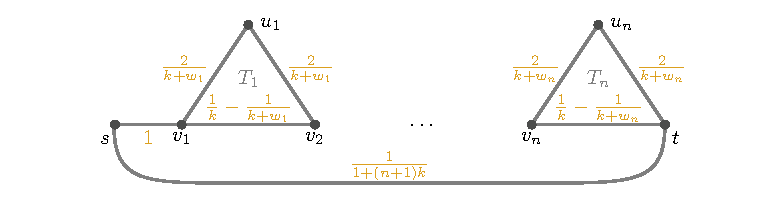
\includegraphics[page=1]
    {switchplacement/figures/hardness_proof.pdf}
    %
    \vspace*{1.3mm}
    \caption[A network constructed from~\gls{ssp}.]{A
    network~\glssymbol{network} constructed from an instance of~\gls{ssp}
    having one source~$\source\in\glssymbol{generators}$ (\ie, $
    \fmagnitude{\glssymbol{generators}}\equiv 1$) and one
    sink~$\sink\in\glssymbol{consumers}$ (\ie, $
    \fmagnitude{\glssymbol{consumers}}\equiv 1$).
    All edges $ (\vertexa,\vertexb)\in\glssymbol{edges}$ have
    a~\screentextcolor{CAPACITY}{capacity}
    of~\screentextcolor{CAPACITY}{$\glssymbol{capacity}\equiv1$} and the
    \screentextcolor{SUSCEPTANCE}{susceptances~\glssymbol{susceptance}}
    are shown next to the edges.}
    %
    \label{ch:switching:sec:complexity:fig:reduction}
\end{figure}
%
%
\begingroup
    \begin{problem}[framed]{\acrlong{ssp}~$\gls{ssp}(W,k)$}
    Instance: & A finite set of numbers~$W=\{w_1,w_2,\dots,w_n\}$
    with~$w_i\in\naturals$ and a~$k\in\naturals$.\\ %
    Question: & Is there a set of elements~$x_1,\dots,x_n\in\{0,1\}$ such that 
    %
    $\sum_{j=1}^{n}w_jx_j = k$?
\end{problem}
    \label{ch:switching:problems:subset-sum-decision-problem}
\endgroup
%
\begin{lemma}
    \kmtsfp\ is~\NP-complete even if there is only one source and one sink in
    the network and all edge capacities are~$1$.
\end{lemma}
% 
\begin{proof}
  We show the~\NP-hardness by reducing~\gls{ssp} to this
  restricted~\gls{mtsfp}-variant in polynomial time. Since~\gls{ssp} is
  % 
  weakly~\NP-complete~\parencite{Gar79}, \gls{mtsfp} is~\NP-hard, too.
 %
 Given an~\gls{ssp}-instance~$(W, k)$ we construct an instance
 of~\gls{mtsfp} that allows a flow of~$2$ if and only if there is a solution
 of the~\gls{ssp}-instance. We may assume without loss of generality that
 no element of~$W$ is larger than~$k$ as these elements are never part of any
 solution. In the constructed network~\glssymbol{network} there is one
 source~$\{\source\}\eqqcolon\glssymbol{generators}$ (\ie, $
 \fmagnitude{\glssymbol{generators}}\equiv 1$) and one sink~$
 \{\sink\}\eqcolon\glssymbol{consumers}$ (\ie, $
 \fmagnitude{\glssymbol{consumers}}\equiv 1$;
 see~\cref{ch:switching:sec:complexity:fig:reduction}). All
 edges~$\edge\in\glssymbol{edges}$ have
 capacity~$\glssymbol{capacity} \equiv 1$. There is one edge from~\source to~\sink
 with susceptance~$\nicefrac{1}{(1+(n+1)k)}$, where~$n=\fmagnitude{W}$. For each
 element~$w_i\in W$ we build a triangle with vertices~$\vertex_i$, $\vertexa_i$,
 and~$\vertex_ {i+1}$. We
 set~$\glssymbol{susceptance}(\vertex_i,\vertexa_i)\coloneqq
 \glssymbol{susceptance}
 (\vertexa_i,\vertex_{i+1})\coloneqq\nicefrac{2}{(k+w_i)}$
 and~$\glssymbol{susceptance}(\vertex_i,\vertex_{i+1})\coloneq\nicefrac{1}{k} -
 \nicefrac{1}{(k+w_i)}$. Note that the triangles for~$w_i$ and~$w_{i+1}$ have
 the vertex~$\vertex_{i+1}$ in common. We set~$v_{n+1}=t$ and add the
 edge~$(\source,\vertex_1)$ with
 susceptance~$\glssymbol{susceptance}(\source,\vertex_1) = 1$. Note that the
 edge~$(\source,\vertex_1)$ is necessary when we do not switch any triangle,
 since this would exceed the flow of one in the upper part.
 
 To achieve a flow of~$2$ in the network both edges incident to~\source must be
 saturated. In particular, the flow through the chain of triangles is~$1$
 and~$\glssymbol{voltageangledifference}(\source,\sink)=1+(n+1)k$. Consider the
 triangle~$T_i$ for the element~$w_i\in W$. In this triangle~$v_i$ acts as a
 source and~$\vertex_{i+1}$ as a sink. There are two paths from~$\vertex_i$
 to~$\vertex_{i+1}$ in~$T_i$: The direct path consisting only of the
 edge~$(\vertex_i,\vertex_{i+1})$ and the path via~$u_i$. In any solution
 to~\glssymbol{network} at most one of these paths may be switched as otherwise
 the total flow in~\glssymbol{network} is at most~$1$. If no edge in~$T_i$ is
 switched
 (\cref{ch:switching:sec:complexity:fig:switching_triangles_hardness}\screen{a}),
 we obtain~$\glssymbol{voltageangledifference}(\vertex_i,\vertex_{i+1})\equiv k$
 for one unit flowing through~$T_i$. If the edge~$(\vertex_i,\vertex_{i+1})$ is
 switched
 (\cref{ch:switching:sec:complexity:fig:switching_triangles_hardness}\screen{b}),
 we have~$\glssymbol{voltageangledifference}( \vertex_i, \vertex_{i+1} ) = k +
 w_i$. If an edge incident to~$\vertexa_i$ is switched
 (\cref{ch:switching:sec:complexity:fig:switching_triangles_hardness}\screen{c}),
 the flow on~$(\vertex_i,\vertex_{i+1})$ must be equal to~$1$ and we get
% 
%%%%%%%%%%%%%%%%%%%%%%%%%%%%%%%%%%%% FIGURE %%%%%%%%%%%%%%%%%%%%%%%%%%%%%%%%%%%
\begin{figure}[tb!]
    \centering
    % 
    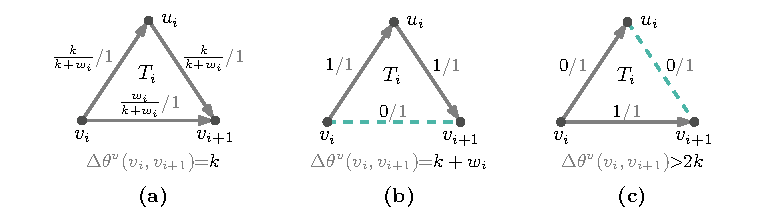
\includegraphics[page=1,trim={0 0.5mm 0 0}, clip]
    {switchplacement/figures/switching_triangles_in_hardness_proof.pdf}
    % 
    \caption[Possible ways to switch in a triangle in a network constructed
    from~\gls{ssp}]{ Possible ways to switch the triangles~$T_i$ in a
    network~\glssymbol{network} with corresponding angle differences and flows.
    (a)~If no edges are switched the angle difference is~$k$. (b)~If the
    edge~$(v_i,v_{i+1})$ is \screentextcolor{KITgreen70}{switched}, the angle
    difference is~$k+w_i$. (c)~If an edge incident to~$u_i$ is
    \screentextcolor{KITgreen70}{switched},
    the angle difference is larger than~$2k$. }
    % 
    \label{ch:switching:sec:complexity:fig:switching_triangles_hardness}
\end{figure}
 % 
 \begin{align*}
  \glssymbol{voltageangledifference}(\vertex_i,\vertex_{i+1})
   = \frac{1}{\frac{1}{k} - \frac{1}{k+w_i}}
   = \frac{k(k+w_i)}{w_i}
   = \frac{k^2}{w_i} + k
   > 2k.
 \end{align*}
 % 
 Note that in any
 case~$\glssymbol{voltageangledifference}(\vertexb_i,\vertexb_{i+1})\geq k$. If
 in any triangle~$T_i$ an edge incident to~$\vertexa_i$ is switched, we have
 % 
 \begin{align*}
  \glssymbol{voltageangledifference}(\source,\sink)
  &= \glssymbol{voltageangledifference}(\source,v_1) + \sum_{i=1}^n 
  \glssymbol{voltageangledifference}(\vertex_i,\vertex_{i+1}) \\
  &> 1 + (n-1)k + 2k
  = 1+ (n+1)k,
 \end{align*}
 % 
 which contradicts~$\glssymbol{voltageangledifference}(\source,\sink)=1+(n+1)k$.
 Hence, only the edges~$(\vertex_i,\vertex_{i+1})$ for~$i=1,\dots,n$ may be
 switched.
 
 If there is a set~\glssymbol{switched} of edges in~\glssymbol{network} such
 that removing them from the network yields a maximum flow~\glssymbol{flow}
 in~$\glssymbol{network}-\glssymbol{switched}$ with
 throughput~$\glssymbol{flowvalue}(\network, \glssymbol{flow}) \equiv 2$, we can
 construct a solution to the corresponding~\gls{ssp}-instance as follows.
 Let~$x_i = 1$ if~$(v_i,v_{i+1})\in
 \glssymbol{switched}$ and~$x_i=0$ otherwise. By the argumentation above we
 have~$\glssymbol{voltageangledifference}(\vertex_i,\vertexb_{i+1}) = k + w_i$
 if~$x_i = 1$ and~$\glssymbol{voltageangledifference}
 (\vertexb_i,\vertexb_{i+1})=k$ otherwise. Hence, we have
 % 
 \begin{align*}
 1+(n+1)k
 &=\glssymbol{voltageangledifference}(\source,\sink)\\
 &= \glssymbol{voltageangledifference}(\source,v_1) 
 + 
 \sum_{i=1}^n\glssymbol{voltageangledifference}(v_i,v_{i+1})\\
 &= 1 + \sum_{i=1}^n(k+x_i w_i)\\
 &= 1 + nk +\sum_{i=1}^n x_i w_i.
 \end{align*}
 % 
 and therefore~$\sum_{i=1}^n x_i w_i = k$ as required by
 the~\gls{ssp}-instance.
 
 If the~\gls{ssp}-instance has a solution, \ie, $\sum_{i=1}^n x_i w_i = k$
 for a suitable assignment of the~$x_i$, we define~$\glssymbol{switched} \coloneqq
 \{
 (\vertexb_i,\vertexb_{i+1}) \mid x_i=1\}$. We claim that after switching these
 edges the remaining network~$\glssymbol{network}-\glssymbol{switched}$ admits a
 power flow with value~$2$. Setting~$\glssymbol{voltageangle}(\source)=0$
 and~$\glssymbol{voltageangle}(\vertexb_i) = 1 + \sum_{j=1}^{i-1}(k + x_i w_i)$
 induces a feasible electrical flow of~$1$ on the triangle chain by the
 arguments above. We further note that
 % 
 \begin{align*}
 \glssymbol{voltageangledifference}(\source,\sink)
 &= \glssymbol{voltageangledifference}(\source,\vertexb_1) + \sum_{i=1}^n\glssymbol{voltageangledifference}(\vertexb_i,\vertexb_{i+1})\\
 &= 1 + \sum_{i=1}^n(k+x_iw_i)\\
 &= 1 + nk + \sum_{i=1}^n x_i w_i\\
 &= 1 + (n+1)k.
 \end{align*}
 % 
 Hence, we have~$\glssymbol{flow}(\source,\sink)\equiv 1$ and the total flow
 in~$\glssymbol{network}-\glssymbol{switched}$ is~$2$.
 
 The size of the constructed network is linear in~$\fmagnitude{W}$ and all
 parameters are polynomial in~$k$. Hence, the reduction from~\gls{ssp}
 to~\gls{mtsfp} runs in polynomial time. Since~\gls{ssp}
 is~\NP-complete~\parencite{Gar79}, this reduction implies that~\gls{mtsfp}
 is~\NP-hard even if we restrict ourselves to networks with unit capacities and
 only one source and one sink.
\end{proof}
% 
%
%%%%%%%%%%%%%%%%%%%%%%%%%%%%%%%%%%%%%%%%%%%%%%%%%%%%%%%%%%%%%%%%%%%%%%%%%%%%%%%
\section{Network Modeling}\label{ch:switching:sec:network_modeling}
%%%%%%%%%%%%%%%%%%%%%%%%%%%%%%%%%%%%%%%%%%%%%%%%%%%%%%%%%%%%%%%%%%%%%%%%%%%%%%%
%
The model presented in~\cref{ch:switching:sec:model} places no restriction on
the network. Our algorithms and proofs are often simpler if the underlying
network has a specific form.
% 
%%%%%%%%%%%%%%%%%%%%%%%%%%%%%%%%%%%% FIGURE %%%%%%%%%%%%%%%%%%%%%%%%%%%%%%%%%%%%
\begin{figure}[t!]%
% 
\centering
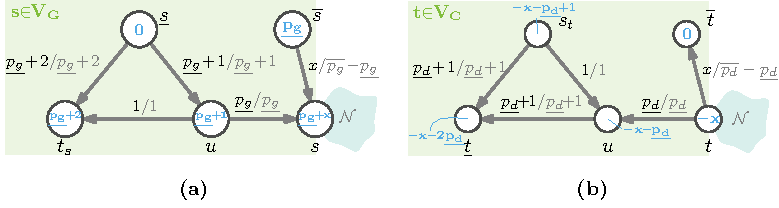
\includegraphics{switchplacement/figures/bounded_unbounded_mtsf_transformation.pdf}%
%
\caption[The transformation of an unbounded into a bounded network.]{
  A bounded network can be transformed to an unbounded network by
  adding substructures to its generator and consumer vertices. (a)~A
  \myhl{KITpalegreen15}{generator~$\source\in\glssymbol{generators}$} in a
  bounded~\gls{mtsfp} can be transformed to a generator in an
  unbounded~\gls{mtsfp} by modifying
  the~\myhl{KITcyanblue15}{network~$\glssymbol{network}$} at the source.
  Thereby, a generator with non-zero lower bound generation can be replaced by a
  construction of a cycle with generator~$\underline{\source}$ and
  consumer~$\sink_{\source}$ forcing a generation
  of~\glssymbol{realpowergenerationmin} on edge~$(\vertexa,\source)$, and a
  generator~$\overline{\source}$ allowing a generation in total of up
  to~\glssymbol{realpowergenerationmax} at vertex~\source.
  (b)~For~\myhl{KITpalegreen15}{consumers~\sink} to model the upper bound it
  suffices to add an edge~$(\overline{\sink},\sink)$ and a minimum demand
  of~\glssymbol{realpowerdemandmin} to~$\overline{\sink}$. To model the lower
  bound, a triangle that configures the voltage angles in such a fashion that
  there is a feasible power flow only if at least the lower demand is satisfied.
  % 
  }
  % 
\label{ch:switching:sec:network_modeling:fig:bounded_unbounded_mtsf_transformation}%
\end{figure}%
%%%%%%%%%%%%%%%%%%%%%%%%%%%%%%%%%%%%%%%%%%%%%%%%%%%%%%%%%%%%%%%%%%%%%%%%%%%%%%%%

Without loss of generality we may assume that in the network
$\glssymbol{network} \coloneqq$ (\glssymbol{graph},
\glssymbol{generators},\glssymbol{consumers}, $\glssymbol{capacity}$,
\glssymbol{susceptance},
\realpowerdemandmin) all generators and consumers are degree\nobreakdash-1
vertices. We achieve this by adding an edge with infinite capacity and a
susceptance of~$1$ between each generator or
consumer~$\vertexb\in(\glssymbol{generators}\cup\glssymbol{consumers})$ and a new
vertex~$\vertexa_{\vertexb}$. The new vertex~$\vertexa_{\vertexb}$ then acts as a
generator or consumer and~\vertexb becomes an intermediate vertex. We use this
assumption especially
in~\cref{ch:switching:sec:exploit_structural_characteristics}, where we restrict
our network to certain graph classes.

We can shrink the network~\glssymbol{network} by contracting degree-2 vertices.
For this we introduce the \emph{susceptance norm} of a path
$\fpath{}{\vertexa}{\vertexb}$, which is defined as
%
\begin{equation}%
    \bnorm{\fpath{}{\vertexa}{\vertexb}}
    \coloneqq
    \sum_{\edge\in\fpath{}{\vertexa}{\vertexb}}
    \glssymbol{susceptance}(\edge)^{-1},
    % 
    \label{eq:bnorm}%
\end{equation}%
% 
and gives us a distance metric on power grids. 
% 
The susceptance norm is a norm, since it fulfills the axioms given
by~\textcite{Ban22}.
% 
\begin{enumerate}
    \item $\norm{\vv{x}}{}\hspace{7.2mm}\equiv 0$ if and only if $\vv{x}\equiv
    \vv{0}$
    (neutral element),
    \item $\norm{ s \cdot \vv{x} }{}\hspace{3mm}\equiv \fmagnitude{s}\cdot\norm{\vv{x}}{}$ 
    \hspace*{21.5mm}(absolute homogeneity),
    \item $\norm{\vv{x}+\vv{y}}{}\leq\norm{\vv{x}}{} + \norm{\vv{y}}{}$ 
    \hspace*{16.5mm}(triangular inequality).
\end{enumerate}
% 
Applying the following lemma we
can simplify~\glssymbol{network} by contracting paths to single edges.
%
%%%%%%%%%%%%%%%%%%%%%%%%%%%%%%%%%% LEMMA %%%%%%%%%%%%%%%%%%%%%%%%%%%%%%%%%
\begin{lemma}%
  A simple path~$\pathu$ in~\glssymbol{network} whose internal vertices have
  degree 2 in~\glssymbol{network} and are neither generators nor consumers is
  equivalent to a single edge~\edge with capacity~$\glssymbol{capacity}
  (\edge)\coloneqq\min_{(\vertexa,\vertexb)\in\pathu}\glssymbol{capacity}
  (\vertexa,\vertexb)$
  and susceptance~$\glssymbol{susceptance}(\edge)\coloneqq\nicefrac{1}{
\bnorm{\pathu}}$.%
\label{ch:switching:sec:network_modeling:lem:series_contraction}
\end{lemma}%
%
Note that if we assume that all generator and consumer vertices have degree 1,
they are never internal vertices of any simple path. Note
that~\cref{ch:switching:sec:network_modeling:lem:series_contraction} is
equivalent to the
transformation~\cref{ch:network-analyzes:sec:mathematical-model:sim:series_contraction}
presented in~\cref{ch:network-analyzes:sec:reduction-transformation-rules}.

\textcite{Leh14,Leh15a} showed that the bounded~\gls{mtsfp} is~\NP-hard on
cacti (\ie, a graph consisting of edge disjoint cycles). We can transform a
bounded~\gls{mtsfp} with network~\dcnetworktuple to an
unbounded~\gls{mtsfp}. We model the upper bounds by adding
edges~$(\vertexa,\vertexb)$ with appropriate capacities at
vertices~$\vertexa\in(\glssymbol{generators}\cup\glssymbol{consumers})$. To
model a
% 
non-zero lower generation bound~$\glssymbol{realpowergenerationmin}$ at a
generator, we replace it by the construction shown
in~\cref{ch:switching:sec:network_modeling:fig:bounded_unbounded_mtsf_transformation}\screen{a},
which is based on a structure used by~\textcite{Leh14}. The cycle with
generator~$\underline{\source}$ and consumer~$\sink_{\source}$
with~$\glssymbol{realpowerdemandmin}(\sink_\source) =
\glssymbol{realpowergenerationmin} + 2$ forces a flow
of~$\glssymbol{realpowergenerationmin}$ on the edge~$(\vertexa,\source)$ and the
generator~$\overline{\source}$ is able to add the remaining generation capacity.
Note that the cycle can be omitted if~$\glssymbol{realpowergenerationmin} \equiv
0$. For consumers we just add an edge~$(\overline{\sink},\sink)$ with a capacity
of~\glssymbol{realpowerdemandmax} to model the upper bound. In addition, the
minimum demand is modeled by a triangle for which the voltage angle
configuration enforces a minimum demand of~\glssymbol{realpowerdemandmin}
(\cref{ch:switching:sec:network_modeling:fig:bounded_unbounded_mtsf_transformation}\screen{b}).
%
\begin{lemma}%
  Every bounded~\gls{mtsfp} can be transformed into an
  unbounded~\gls{mtsfp} on a network with size linear
  in~$\fmagnitude{\glssymbol{vertices}}$ and~$\fmagnitude{\glssymbol{edges}}$.
  % 
  \label{lem:bounded_unbounded_mtsf_transformation}%
\end{lemma}%
%%%%%%%%%%%%%%%%%%%%%%%%%%%%%%%%%%%% FIGURE %%%%%%%%%%%%%%%%%%%%%%%%%%%%%%%%%%%%
\begin{figure}[t!]%
  \centering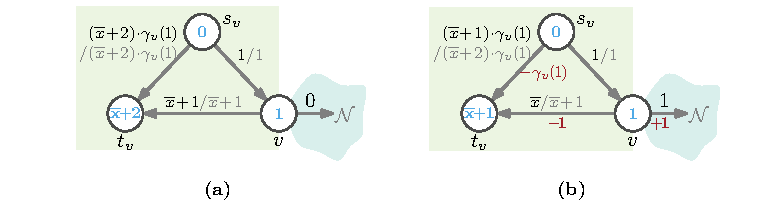
\includegraphics{switchplacement/figures/ots_mtsf_transformation.pdf}
  %
  \caption[Transformation from an~\gls{otsp}- to an~\gls{mtsfp}-instance.]{
    Transforming an~\gls{otsp}-instance to an~\gls{mtsfp}-instance is
    possible by adding triangles at consumer vertices. The
    edge~$\edge=(\source_\vertex,\sink_\vertex)$ and the other two edges have
    susceptances~$\glssymbol{susceptance}(\edge)=\cost_\vertex(1)$ and~$1$,
    respectively. (a)~The maximum flow in a triangle is obtained by injecting no
    power to the network~\glssymbol{network} from~\vertex. (b)~Per injected unit
    of flow from~\vertex to~\glssymbol{network}, there is a decrease in flow
    value by~$\cost_\vertex(1)$ (\textcolor{KITred}{red}) in a triangle.}
  % 
  \label{fig:ots_mtsf_transformation}%
\end{figure}%
%
%
\textcite[Lemma 2]{Leh14} show that
every~\gls{mtsfp}-instance can be transformed to an equivalent
\gls{otsp}-instance while maintaining the network structure. The idea is
basically that we pay for each unit a consumer is not used to its maximum
capacity~\glssymbol{realpowerdemandmax}
meaning~$\glssymbol{realpowerdemandmax}(\vertexa)-\glssymbol{netflow}
(\vertexa)\neq 0$ and we
pay~$\fmagnitude{\glssymbol{realpowerdemandmax}(\vertexa)-\glssymbol{netflow}
(\vertexa)}$ units. This transformation is done by defining a generator cost
function~$\gamma\colon\glssymbol{generators}\cup\glssymbol{generators}'\to\posreals$
with~$\vertexa\in\glssymbol{generators}'$ if~$\vertexa\in\glssymbol{consumers}$
and~$\gamma_\vertexa (1)\equiv 1$ with~$\vertexa\in\glssymbol{generators}'$
and~$\gamma_\vertexa(1)\equiv 0$ for all~$\vertexa\in\glssymbol{generators}$. In
addition, the consumptions are fixed
meaning~$\glssymbol{realpowerdemandmin}(\vertexa) =
\glssymbol{realpowerdemandmax}(\vertexa) =
\glssymbol{realpowerdemand}(\vertexa)$ for all~$\vertexa\in\glssymbol{consumers}$. Thus, while
maximizing the power flow a generator~$\vertexa\in\glssymbol{generators}'$
produces~$\glssymbol{realpowerdemandmax}(\vertexa)-\glssymbol{netflow}(\vertexa)$ units of
flow.

We present the reverse transformation for
\gls{otsp} with linear cost functions. Let~\dcnetworktuple be a bounded
network, where each consumer~$\vertex\in\glssymbol{consumers}$ has a fixed
demand~$\glssymbol{realpowerdemand}(\vertex) =
\glssymbol{realpowerdemandmin}(\vertex) =
\glssymbol{realpowerdemandmax}(\vertex)$. At each
generator~$\vertex\in\glssymbol{generators}$ with cost~$\cost_{\vertex}(1)$ per
generated unit of power we add a triangle consisting of~\vertex, another
generator~$\source_{\vertex}$ and a consumer~$\sink_{\vertex}$ as shown
in~\cref{fig:ots_mtsf_transformation}. The
edge~$(\source_\vertex,\sink_\vertex)$ has susceptance~$\cost_{\vertex}(1)$ and
the other two edges have susceptance~$1$. We denote the resulting network
by~$\glssymbol{network}'$.
%
If~$\vertex$ injects no power into the original network
(\cref{fig:ots_mtsf_transformation}\screen{a}), all its generated power flows
along~$(\vertex, \sink_\vertex)$ to~$\sink_\vertex$. The flow in this triangle
is then maximized by sending $1$ unit from $\source_{\vertex}$ via~\vertex to
$\sink_\vertex$ and $(\maxexcess_\vertex+2)\cdot\cost_{\vertex}(1)$ units
directly on $(\source_\vertex, \sink_\vertex)$. Per unit of flow injected
by~\vertex into the original network, the angle difference
$\glssymbol{voltageangledifference}(\vertex, \sink_{\vertex})$ decreases by~$1$
(\cref{fig:ots_mtsf_transformation}\screen{b}). Therefore,
$\glssymbol{voltageangledifference}(\source_\vertex, \sink_\vertex)$ also
decreases by $1$ and the flow~$\glssymbol{flow}(\source_\vertex,
\sink_{\vertex})$ by~$\cost_\vertex(1)$. Hence, a feasible flow
in~$\glssymbol{network}$ with cost~$k$ can be transformed to a feasible flow
in~$\glssymbol{network}'$ with flow value~$M-k$, where~$
M
=
\sum_{\vertex\in\glssymbol{generators}}
\left((\glssymbol{realpowergenerationmax}(\vertex)+2)\cdot\cost_\vertex(1)
+
\glssymbol{realpowergenerationmax}(\vertex) + 1\right)
% 
$. This leads to the following lemma.
% 
\begin{lemma}
    \label{lem:ots_msf_transformation}
    For every~\gls{otsp}-instance~\dcnetworktuple with fixed
    demands~$\glssymbol{realpowerdemand}(\vertex) =
    \glssymbol{realpowerdemandmin}(\vertex) =
    \glssymbol{realpowerdemandmax}(\vertex)$ and linear cost
    functions~$\cost_{\vertex}$ for each
    consumer~$\vertex\in\glssymbol{consumers}$ there is
    an~\gls{mtsfp}-instance~$\glssymbol{network}'$ and a
    constant~$M\in\posreals$ such that for every~$k\in\posreals$ we
    have~$\opt_{\gls{otsp}}(\glssymbol{network})\le k$ if and only
    if~$\opt_{\gls{mtsfp}}(\glssymbol{network}')\ge M-k$. Moreover, the size
    of~$\glssymbol{network}'$ is linear in the size of~\glssymbol{network}.
% 
\end{lemma}
% 
The previous lemma and the result of~\textcite[Lemma 2]{Leh14} provide a
possibility to interchangeably apply algorithms found for~\gls{mtsfp}
to~\gls{otsp} (and vice versa) by a simple graph transformation.

% 
%%%%%%%%%%%%%%%%%%%%%%%%%%%%%%%%%%%%%%%%%%%%%%%%%%%%%%%%%%%%%%%%%%%%%%%%%%%%%%%
\section{MTSF on Source-Sink-Networks}
\label{ch:switching:sec:exploit_structural_characteristics}
%%%%%%%%%%%%%%%%%%%%%%%%%%%%%%%%%%%%%%%%%%%%%%%%%%%%%%%%%%%%%%%%%%%%%%%%%%%%%%%
%
\textcite{Fis08} found in their experiments that \emph{Wheatstone Bridges}
\parencite{905717} (bridges or short-cut edges in a cycle with four edges) can
be associated with \emph{Braess's Paradox}~\parencite{Bra05,Pal12,Nag10}, in
which adding a line to a network (even with zero cost) can increase the cost of
using that network
(see~\cref{ch:related-work:sec:braess-paradox}).
These structures are often removed by switches in their results. In the
following, we denote Wheatstone Bridges by
%
\emph{cycle
chords}~\parencite[p.~225]{online:ISGCI:Information_System_on_Graph_Class_Inclusions:V2_0,west_introduction_2000},
since a \emph{bridge} in a graph is an edge whose removal disconnects the graph,
which is not what we mean here.
%
The structure---meaning cycle and chord together---is denoted by \emph{diamond
graph}. An observation of~\textcite{Fis08} is the following.
%
%%%%%%%%%%%%%%%%%%%%%%%%%%%%%%%%%%   LEMMA %%%%%%%%%%%%%%%%%%%%%%%%%%%%%%%%
\begin{observation}
    The~\gls{otsp} and thus the~\gls{mtsfp} try to remove an edge
    set~\gls{switched} in such a way that the remaining graph is often
    chordless.
    % 
    \label{obs:wheatstone_bridges}
\end{observation}
%
We will show in this section that~\cref{obs:wheatstone_bridges} does not apply
in general. However, \textcite{Fis08} empirically show on their test case that
this is often the case. \textcite{Lei15b} prove that placing ideal~\gls{facts}
in such a way that the remaining grid is a tree results in a~\gls{mpf}, which is
equivalent to the~\gls{mf}. This observation indicates that the power flow is
equivalent to the graph theoretical flow on trees as only determined by the
conservation of flow
(\gls{kcl},~\cref{ch:switching:sec:model:eq:flow_conservation})~\parencite[see][Lemma~4]{Leh15a}.
However, power grids are meshed (\ie, they contain cycles) for reliability
reasons. Each mesh in a power grid has to obey the~\gls{kvl}
(\cref{ch:switching:sec:model:eq:KVL_dc_approx}), meaning the sum of all voltage
angle differences is zero. These additional constraints are not only the
difference to a graph-theoretical flow, but make most of the problems hard to
solve even in the~\gls{dc} model. In addition, they lead to~Braess's Paradox and
make switching beneficial
(see~\cref{ch:related-work:sec:braess-paradox}).

The idea is to reach a graph-theoretical flow by exploiting the network
structure~\glssymbol{network}. The upper and lower bound for~\gls{mtsf}
are given by~$\opt_{\gls{mfp}}$ and~$\opt_{\gls{mpfp}}$, respectively.
%
%%%%%%%%%%%%%%%%%%%%%%%%%%%%%%%%%%%% LEMMA %%%%%%%%%%%%%%%%%%%%%%%%%%%%%%%%%%%%
\begin{lemma}
    $\opt_{\gls{mpfp}}\leq\opt_{\gls{mtsfp}}\leq\opt_{\gls{mfp}}$.
    % 
    \label{lem:opt_relation_mpf_msf_mf}
\end{lemma}
%
Transmission switching problems formulated as~\gls{milp} models have highly
coupled constraints~(see~\cref{ch:switching:sec:model}). Cycles
add~\gls{kvl} constraints (\cref{ch:switching:sec:model:eq:KVL_dc_approx})
to the problem, which are highly coupled with each other as the sum over the
voltage angle differences in each cycle has to be zero
(\cref{ch:switching:sec:model:fig:simple_switching_example}). Thus, we get the
following observation.
%s
%%%%%%%%%%%%%%%%%%%%%%%%%%%%%%%%%% OBSERVATION %%%%%%%%%%%%%%%%%%%%%%%%%%%%%%%%%
\begin{observation}%
  The relation~$\opt_{\gls{mpfp}} < \opt_{\gls{mfp}}$ can only be caused
  by cycles.
  %
  \label{obs:complex_cycles}
\end{observation}%
%
In this section we study~\gls{mtsfp} on networks that have only one 
generator vertex~\source and one consumer vertex~\sink. We call such 
networks~\emph{\source-\sink-networks}.
% 
Let~$\paths(\vertexa,\vertexb)$ denote
the set of all paths between two vertices~\vertexa and~\vertexb. We denote
the smallest capacity of any edge on a
path~$\pathu\in\paths(\vertexa,\vertexb)$ by
%
%%%%%%%%%%%%%%%%%%%%%%%%%%%%%%%%%%%%  EQUATI%%%%%%%%%%%%%%%%%%%%%%%%%%%%%%%%%%%
\begin{align}%
    \fmincapacity{}{\pathu}\coloneqq
    \min_{(\vertexa,\vertexb)\in\pathu}
    \fcapacity{}{\vertexa}{\vertexb}.
    % 
    \label{eq:edge_min_capacity}
    % 
\end{align}%
%  

From~\cref{ch:switching:sec:model:eq:capacity_constraints,ch:switching:sec:model:eq:KVL_dc_approx}
we get the following function to calculate the maximum voltage angle difference
on any~\vertexa-\vertexb-path~$\fpath{}{\vertexa}{\vertexb}\in\paths
(\vertexa,\vertexb)$.
% 
\begin{align}
    % 
    \glssymbol{voltageangledifference}(\fpath{}{\vertexa}{\vertexb})&
    \coloneqq\!
    \bnorm{\fpath{}{\vertexa}{\vertexb}}\cdot\fmincapacity{}{\fpath{}
      {\vertexa}{\vertexb}}.
    % 
    \label{eq:update_function}
    % 
\end{align}
% 
% 
For~$\fpath{1}{\vertexa}{\vertexb},$
$\fpath{2}{\vertexa}{\vertexb}\in\paths(\vertexa,\vertexb)$ we
define~$\fpath{1}{\vertexa}{\vertexb}\leq\fpath{2}{\vertexa}{\vertexb}$
if and only if~$\glssymbol{voltageangledifference}(\fpath{1}{\vertexa}{\vertexb})$ 
$\leq\glssymbol{voltageangledifference}(\fpath{2}{\vertexa}{\vertexb})$.
% 
%%%%%%%%%%%%%%%%%%%%%%%%%%%%%%%%%%%%%%%%%%%%%%%%%%%%%%%%%%%%%%%%%%%%%%%%%%%%%%%%
\subsection{The Dominating Theta Path (DTP)}
\label{ch:switching:sec:exploit_structural_characteristics:subsec:dtp}
%%%%%%%%%%%%%%%%%%%%%%%%%%%%%%%%%%%%%%%%%%%%%%%%%%%%%%%%%%%%%%%%%%%%%%%%%%%%%%%%
% 
The intuition that electricity follows the path of the least resistance leads us
towards shortest paths. However, in power grids the shortest path is not always
the restricting path.%
%
%%%%%%%%%%%%%%%%%%%%%%%%%%%%%%%%%%%% FIGURE %%%%%%%%%%%%%%%%%%%%%%%%%%%%%%%%%%%%
\begin{figure}[tb!]
    \centering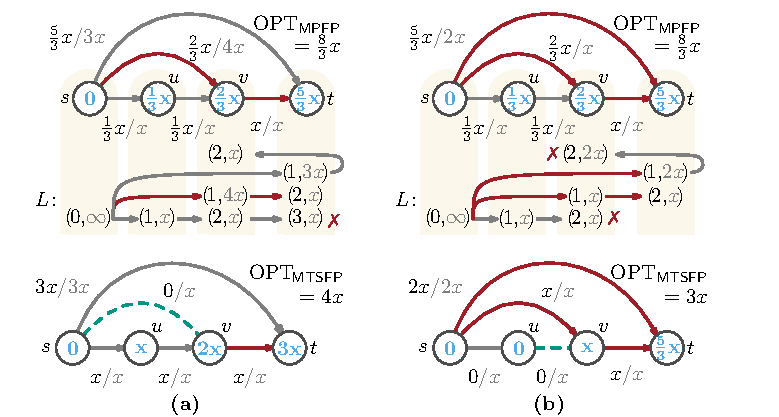
\includegraphics{switchplacement/figures/comparing_delta_theta_path.pdf}
    %
    \caption[An example and counterexample for the~\gls{dtp} calculation.]
    {%
    A network~\glssymbol{network} with four vertices and five edges, one
    generator~$\glssymbol{generators}=\{\source\}$, one
    consumer~$\glssymbol{consumers}=\{\sink\}$,
    capacities~\screentextcolor{KITblack50}{$\capacity(\vertexa,\vertexb)$}
    \mbox{(\screentextcolor{KITblack50}{gray})}, susceptance~$\glssymbol{susceptance}
    (\vertexa,\vertexb)=1$ for all $(\vertexa,\vertexb)\in\glssymbol{edges}$,
    and voltage angles~\screentextcolor{THETA}{$\vangle(\vertexa)$}
    (\screentextcolor{THETA}{blue} in the vertices) for all
    vertices~$\vertexa\in\vertices$. Note for the label calculation that the
    underlying graph~\graph is undirected. The algorithm computing the~\gls{dtp}
    saves a set of labels~\myhl{HiLi!50}{$\glssymbol{labels}$} for each vertex
    starting at vertex~\source with label~$(0,\infty)$. The 
    \screentextcolor{KITred}{red edges} represent the~\gls{dtp} from~\source
    to~\sink. (a)~The cross~\screentextcolor{KITred}{\ding{55}} means that the
    label~$(3,x)$ is dominated by the label~$(2,x)$ at vertex~\sink. In
    addition, it is not sufficient to compare only the voltage angle
    differences~\glssymbol{voltageangledifference}, since we would drop
    the~\gls{dtp} path~$[\source, (\source,\vertexb),\vertexb]$ at
    vertex~\vertexb, which would lead to incorrect results. Switching
    edge~$(\source,\vertexb)$ (\screentextcolor{KITgreen}{green dashed edge})
    results in a solution of the~\gls{mtsfp}. (b)~The~\gls{dtp} is not always
    unique. In addition, for general graphs the switched edge of the~\gls{mtsfp}
    is not always on the~\gls{dtp}. }%
    % 
    \label{fig:comparing_delta_theta_path} 
\end{figure}
% 
An~\source-\sink-network is often restricted (dominated) by the path with
the smallest voltage angle difference. However, it does not seem feasible to
give a general bound for that. %
The smallest voltage angle difference between a vertex~\vertexa and a
vertex~\vertexb is denoted by~$\glssymbol{voltageangledifferencemin}(\vertexa,\vertexb) \coloneqq
\min\glssymbol{voltageangledifference}\left(\fpath{}{\vertexa}
{\vertexb}\right)$ with $
\fpath{}{\vertexa}{\vertexb}\in\paths(\vertexa,\vertexb)$. 
% 
% 
We call the path that minimizes~$\glssymbol{voltageangledifference}(\fpath{}{\vertexa}{\vertexb})$
\acrlong{dtp} (\gls{dtp}) and denote it by~$\fpath{\dtp}{\vertexa}
{\vertexb}$. Its
value is
denoted by~$\opt_{\gls{dtp}}(\vertexa,\vertexb)$. 
%  
%
We are mainly interested in~\source-\sink-paths, since the power flows from
generators~\source to consumers~\sink.
% 
%%%%%%%%%%%%%%%%%%%%%%%%%%%%%%%%%% ALGORITHM %%%%%%%%%%%%%%%%%%%%%%%%%%%%%%%%%%%
%
% \wormhole{bit:ch:switching:sec:exploit_structural_characteristics:subsec:dtp:alg:shortest_theta_path}
\def\HiLi{\leavevmode\rlap{\hbox to \hsize{\color{HiLi}\leaders\hrule
height .9\baselineskip depth 1.3ex\hfill}}}
\begin{algorithm}[tb!]%
\SetAlgoLined
  % 
  % 
  \KwData{A network~$\glssymbol{network} = 
  (\glssymbol{graph},\glssymbol{generators},\glssymbol{consumers},\glssymbol{capacity},\glssymbol{susceptance})$.}
  % 
  \KwResult{$\fpath{\glssymbol{dtp}}{\source}{\sink}$,
  $\glssymbol{voltageangledifferencemin}(\source,t)$, and
  $\glssymbol{paretolabels}(\vertex)$ with~$\vertex\in\glssymbol{vertices}$.}
  % 
  % INITIALIZATION %%%%%%%%%%%%%%%%%%%%%%%%%%%%%%%%%%%%%%%%%%%%%%%%%%%%%%%%%%%%
  $\glssymbol{paretolabels}(\vertexa) \coloneqq \glssymbol{labels}(\vertexa)
  \coloneqq
  \emptyset \hspace{1em}\forall\vertexa\in\glssymbol{vertices}$%
  \Comment*{\color{KITblack30}Initialization}%
  \label{alg:initialization_begin}
  
  $\glssymbol{priorityqueue}\coloneqq\emptyset$\;
  
  $\glssymbol{labels}(\source) \coloneqq \left\{(0, \infty)\right\}$%
  \Comment*{\color{KITblack30} Special label for source~$\source$}%
  \label{ch:switching:sec:exploit_structural_characteristics:subsec:dtp:alg:shortest_theta_path:line:source_init}

  \screen{\HiLi}
  $\glssymbol{priorityqueue}.\myinsert\big((0,\infty),\source,\mathrm{key}((0,\infty))\big)$\; 
  \label{alg:initialization_end}
  %
  % LOOP UNTIL QUEUE IS EMPTY %%%%%%%%%%%%%%%%%%%%%%%%%%%%%%%%%%%%%%%%%%%%%%%%%
  \While(\Comment*[f]{\color{KITblack30}Visit all
  vertices}){$\glssymbol{priorityqueue}\not=\emptyset$} { % while
    % $\vertices:=\vertices\setminus\{\vertexa\}$\;
    %
    $(\glssymbol{label},\vertexa,\mathrm{key}) \coloneqq \glssymbol{priorityqueue}.\deleteMin()$\;
    \label{ch:switching:sec:exploit_structural_characteristics:subsec:dtp:alg:shortest_theta_path:line:min_key}
    $\glssymbol{paretolabels}(\vertexa) \coloneqq
    \glssymbol{paretolabels}(\vertexa) \cup \{
    \glssymbol{label} \}$\;
    \label{ch:switching:sec:exploit_structural_characteristics:subsec:dtp:alg:shortest_theta_path:line:paretolabels}
    % UPDATE ADJACENT VERTICES %%%%%%%%%%%%%%%%%%%%%%%%%%%%%%%%%%%%%%%%%%%%%%%%
    \For(\Comment*[f]{\color{KITblack30}Check adjacent vertices}){$\forall
    \{\vertexa,\vertexb\}\in\glssymbol{undirectededges}$
    \label{alg:check_adjacent_vertices}}{
    % 
      % MODIFIED UPDATE FUNCTION %%%%%%%%%%%%%%%%%%%%%%%%%%%%%%%%%%%%%%%%%%%%%%
      $\fmincapacity{}{\fpath{}{\source}{\vertexa,\vertexb}} \coloneqq
      \min\left(\glssymbol{label}[1],
      \capacity(\vertexa,\vertexb)
      \right)$\;
      % 
      \def\HiLi{\leavevmode\rlap{\hbox to \hsize{\color{HiLi}\leaders\hrule
      height 1.\baselineskip depth 1.70ex\hfill}}}
      \screen{\HiLi}
      $\labnew(\vertexb)\coloneqq\left(\glssymbol{label} [0]
            +\frac{1}{\glssymbol{susceptance}(\vertexa,\vertexb)},\fmincapacity{}{
                  \fpath{}{\source}{\vertexa,\vertexb}}\right)$\;
      % 
      \label{ch:switching:sec:exploit_structural_characteristics:subsec:dtp:alg:shortest_theta_path:line:update_function_alg}
      %
      % DECIDE WETHER UPDATE OR NOT %%%%%%%%%%%%%%%%%%%%%%%%%%%%%%%%%%%%%%%%%
      \def\HiLi{\leavevmode\rlap{\hbox to \hsize{\color{HiLi}\leaders\hrule
      height .8\baselineskip depth 1.3ex\hfill}}}
      \screen{\HiLi}
      \If{$\isReachable(\glssymbol{vertices}\setminus\{\vertexb\},\glssymbol{label},\source)$
        \label{ch:switching:sec:exploit_structural_characteristics:subsec:dtp:alg:shortest_theta_path:line:check_reachability}}
      {
        \uIf{$\labnew(\vertexb)\in\glssymbol{labels}(\vertexb)$
          \label{ch:switching:sec:exploit_structural_characteristics:subsec:dtp:alg:shortest_theta_path:line:check}}{
          $\parent(\labnew(\vertexb)) \coloneqq \parent(\labnew(\vertexb)) \cup 
          \{\glssymbol{label}\}$\;
        }
        \ElseIf{\kwnot $\glssymbol{labels}(\vertexb)$ \kwdominates $\labnew(\vertexb)$ 
          \label{ch:switching:sec:exploit_structural_characteristics:subsec:dtp:alg:shortest_theta_path:line:check_dominance}}
        {
          $\glssymbol{labels}(\vertexb).\deleteDominatedLabels(\labnew(\vertexb))$\;
          $\glssymbol{priorityqueue}.\deleteDominatedLabels(\labnew(\vertexb), \vertexb)$\;
            \label{ch:switching:sec:exploit_structural_characteristics:subsec:dtp:alg:shortest_theta_path:line:delete_dominated_Q}
          $\glssymbol{labels}(\vertexb).\myinsert(\labnew(\vertexb))$\;
            \label{ch:switching:sec:exploit_structural_characteristics:subsec:dtp:alg:shortest_theta_path:line:insert_L}
          $\glssymbol{priorityqueue}.\myinsert(\labnew(\vertexb),\vertexb,
            \mathrm{key}(\labnew(\vertexb)))$\;
            \label{ch:switching:sec:exploit_structural_characteristics:subsec:dtp:alg:shortest_theta_path:line:insert_Q}
          $\parent(\labnew(\vertexb)) \coloneqq \{\glssymbol{label}\}$\;
        } % else if
      } % if
    } % for
  } \vspace{-2mm} % while
  \Return{\hspace{-.08cm}$
    \left (
      \begin{tabular}{l}
      $\!\!\!\!\!\!~\fpath{\glssymbol{dtp}}{\source}{\sink}\coloneqq\getPaths
      (\source,\sink),\,\,$\Comment{
      \color{KITblack30}Build paths from \parent\hphantom{-}\!\!\!\!\!}\\ 
      $\!\!\!\!\glssymbol{voltageangledifferencemin}(\source,t)\coloneqq 
      \min_{\glssymbol{label}\in\glssymbol{paretolabels}(\sink)}\{\glssymbol{label}
      [0]\cdot\glssymbol{label} [1]\},\!\!\!$\\      % $\tree_{\dtp}:=\parent(\cdot),$ 
      $\!\!\!\glssymbol{paretolabels}(\cdot)$
      \end{tabular}
    \right )
  $
  }\;
  \caption{\acrlong{dtp}~(\gls{dtp}) Algorithm}%
\label{ch:switching:sec:exploit_structural_characteristics:subsec:dtp:alg:shortest_theta_path}%
\end{algorithm}% 
% 

Note that, unlike shortest paths, a~\gls{dtp} from~\source to~\sink via another
vertex~\vertexb and a~\gls{dtp} from~\source to~\vertexb may have no common
edges. For example in the top part
of~\cref{fig:comparing_delta_theta_path}\screen{a} a~\gls{dtp} to~\vertexb goes
via~\vertexa, but not the~\gls{dtp} to~\sink. To compute a~\gls{dtp} we
therefore minimize over two objectives~$\bnorm{\cdot}$
and~$\glssymbol{mincapacity}(\cdot)$. For this we perform a multi-objective
search, where we search for Pareto-optimal solutions, \ie, we look for paths
that are not dominated by other paths with regards to the objective functions
(in our case the susceptance norm~$\bnorm{\cdot}$ and minimum
capacity~$\glssymbol{mincapacity}(\cdot)$). Note that in general multi-objective
search is already~\NP-hard for two objective functions~\parencite{Gar79}
(see~\cref{ch:switching:sec:exploit_structural_characteristics:subsec:dtp:fig:non_poly_number_of_labels}).
%
\begin{definition}[Label Domination Criteria]
    % 
    Each~\source-\vertexa-path~$\pathu$ in~\glssymbol{network} defines a
    label~$\lab=(\bnorm{\pathu},\glssymbol{mincapacity}(\pathu))$ at~\vertexa.
    % 
    A label~$(\bnorm{\pathu_1}, \glssymbol{mincapacity}(\pathu_1))$
    \emph{dominates} another label~$(\bnorm{\pathu_2},
    \glssymbol{mincapacity}(\pathu_2))$ if
    $\bnorm{\pathu_1}\leq\bnorm{\pathu_2}$ and
    $\glssymbol{mincapacity}(\pathu_1)\le\glssymbol{mincapacity}(\pathu_2)$. 
    % 
\end{definition}
% 
% 
The Pareto set~$\glssymbol{paretolabels}(\vertexa)$ of labels at a
vertex~$\vertexa\in\glssymbol{vertices}$ is then defined as the set of
nondominated labels of all~\source-\vertexa-paths
(\cref{ch:switching:sec:exploit_structural_characteristics:subsec:dtp:alg:shortest_theta_path:line:paretolabels}).
%
These Pareto sets can be computed by a natural extension of Dijkstra's algorithm
(see~\cref{ch:switching:sec:exploit_structural_characteristics:subsec:dtp:alg:shortest_theta_path})
known as the
% 
\emph{multi-criteria shortest-path} algorithm~\parencite{MARTINS1984236}. At
each vertex~$\vertexa\in\glssymbol{vertices}$ a set of nondominated labels~$
\glssymbol{labels}(\vertexa)$
% 
is stored. Note that in general, each label may correspond to 
% 
multiple~\source-\vertexa-paths. As it is necessary to represent all these
paths, we store for each label a set of~\parent-pointers. The latter point to
labels that correspond to paths shortened by one vertex. The merging of labels
ensures the polynomial size of label sets.

%
The labels in the priority queue~\glssymbol{priorityqueue} are compared
by~$\bnorm{\cdot}$.
% 
% 
At the beginning of each iteration a label with the minimum susceptance norm is
extracted from~\glssymbol{priorityqueue}. This label belongs to a
vertex~\vertexa. Then, new labels for all neighbors of~\vertexa are computed
(\cref{ch:switching:sec:exploit_structural_characteristics:subsec:dtp:alg:shortest_theta_path:line:update_function_alg}). First, it is checked
whether there is a path~$\fpath{}{\source}{\vertexa}$ that corresponds to~
\glssymbol{label} and does not contain the neighbor~\vertexb
(\cref{ch:switching:sec:exploit_structural_characteristics:subsec:dtp:alg:shortest_theta_path:line:check_reachability},
\cref{ch:switching:sec:exploit_structural_characteristics:subsec:reachibility_test}). Extending this path to~\vertexb then
still gives a simple path. If the computed label already exists
in~$\glssymbol{labels}(\vertexb)$, the~\parent-pointers are updated. Otherwise,
if it is not dominated, it is added to~$\glssymbol{labels}(\vertexb)$
and~\glssymbol{priorityqueue}
(\cref{ch:switching:sec:exploit_structural_characteristics:subsec:dtp:alg:shortest_theta_path:line:insert_L,ch:switching:sec:exploit_structural_characteristics:subsec:dtp:alg:shortest_theta_path:line:insert_Q}).
Before that, all labels dominated by the new labels are removed. Here, only
labels at the same vertex are considered, \ie, in
\cref{ch:switching:sec:exploit_structural_characteristics:subsec:dtp:alg:shortest_theta_path:line:delete_dominated_Q} only the dominated labels
at~\vertexb are removed.
%
\begin{lemma}%
\cref{ch:switching:sec:exploit_structural_characteristics:subsec:dtp:alg:shortest_theta_path} computes a correct~\acrlong{dtp}~(\gls{dtp}).
\label{lem:correctDTP}
\end{lemma}%
% 
Note that the proof for the next lemma is based on the proof for the 
\emph{multi-criteria shortest-path} algorithm by~\textcite{MARTINS1984236}.
% 
\begin{proof}
    At any step of~\cref{ch:switching:sec:exploit_structural_characteristics:subsec:dtp:alg:shortest_theta_path} there is a set of
    labels~$\glssymbol{labels}(\vertexa)$ associated with each vertex
    $\vertexa\in\glssymbol{vertices}$. We first show that at any step no label
    in~$\glssymbol{labels}(\vertexa)$ is dominated by any other label in the same
    set.
    %
    % Base case
    %
    After the initialization there is only one label. Hence, it is not
    dominated. 
    %
    % Induction step 
    %
    %%%%%%%%%%%%%%%%%%%%%%%%%%%%%%%%%% FIGURE %%%%%%%%%%%%%%%%%%%%%%%%%%%%%%%%%%
    \begin{figure}
    % 
    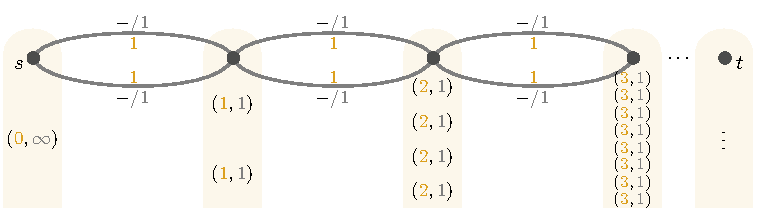
\includegraphics[page=1]{switchplacement/figures/DTP_non_poly_num_labels.pdf}
    % 
    \caption[An example, where the~\gls{dtp} produces exponential many labels.]
    {%
    An example, where the~\gls{dtp} produces exponential many labels. The edges
    are given with
    the~\textcolor{SUSCEPTANCE}{susceptances~\glssymbol{susceptance}} and
    \textcolor{CAPACITY}{capacities~\glssymbol{capacity}}. The sets of labels
    are marked at the vertices. The number of labels increases from the
    source~\source for each vertex in the chain exponentially by either choosing
    the upper or lower edge.
    }%
    % 
    \label{ch:switching:sec:exploit_structural_characteristics:subsec:dtp:fig:non_poly_number_of_labels}
    % 
    \end{figure}
     
    Suppose that there are no dominated labels in any label set before an iteration.
    We show that this property still holds after the iteration.
    First, a label~$(\bnorm{\fpath{}{\source}{\vertexa}},$ 
    $\glssymbol{mincapacity}(\fpath{}{\source}{\vertexa}))$ with the 
    minimum susceptance norm among all labels in~\glssymbol{priorityqueue} is
    dequeued (\cref{ch:switching:sec:exploit_structural_characteristics:subsec:dtp:alg:shortest_theta_path:line:min_key}). This label
    corresponds to a path~$\fpath{}{\source}{\vertexa}$ from~\source 
    to~\vertexa. Then, the labels for neighbors of~\vertexa are computed
    (\cref{ch:switching:sec:exploit_structural_characteristics:subsec:dtp:alg:shortest_theta_path:line:update_function_alg} based
    on~\cref{eq:update_function}). Since these labels are only added if they are
    not dominated and labels dominated by them are removed
    from~$\glssymbol{labels}(\vertexb)$, the label sets still do not contain
    dominated labels. Moreover, the new labels also correspond to simple paths
    as it is tested whether~\vertex already lies
    on~$\fpath{}{\source}{\vertexa}$. Note that previously extracted labels
    from~\glssymbol{priorityqueue} are not removed since their susceptance norm
    is less than the one of~$\lab_\textrm{new}(\vertexb)$. In particular, all
    labels extracted from~\glssymbol{priorityqueue} will be present in the final
    label sets.

    Secondly, we prove that in the end we have~$\glssymbol{paretolabels}
    (\vertexb)\subseteq\glssymbol{labels}(\vertexb)$ for
    all~$\vertexb\in\glssymbol{vertices}$. Assume that this was not the case.
    Then, there is a label~$\lab\in\glssymbol{paretolabels}(\vertexb)$ that is
    not included in~$\glssymbol{labels} (\vertexb)$ for
    some~$\vertexb\in\glssymbol{vertices}$. We pick such a label with the
    minimum susceptance norm. This label corresponds to a path~$\pathu(\source,
    \vertexb)$. Denote the vertex before~\vertexb by~\vertexa. 
    Since the subpath~$\pathu(\source, \vertexa)$ from~$\source$ to~$\vertexa$ has~$
    \bnorm{\pathu(\source,\vertexa)} < \bnorm{\pathu(\source,\vertexb)}$, the 
    label for this subpath is present in~$\glssymbol{labels}(\vertexa)$. But in the
    iteration in which this label was processed, all neighbors of~\vertexa were
    explored. In particular, the label~\lab for~\vertexb was computed and added
    to~$\glssymbol{labels}(\vertexb)$. Moreover, it was never removed
    from~$\glssymbol{labels}(\vertexb)$ later, since it is not dominated. This
    contradicts the existence of~\lab.
    % 
    Since~$\glssymbol{paretolabels}(\vertexa)\subseteq\glssymbol{labels}(\vertexa)$
    and~$\glssymbol{labels}(\vertexa)$ contains no dominated labels, we
    conclude~$\glssymbol{paretolabels}(\vertexa)=\glssymbol{labels}(\vertexa)$.
    The~\gls{dtp} is then computed by minimizing
    over~$\glssymbol{labels}(\sink)$.
\end{proof}
% 
%%%%%%%%%%%%%%%%%%%%%%%%%%%%%%%%%% FIGURE %%%%%%%%%%%%%%%%%%%%%%%%%%%%%%%%%%
\begin{figure}[tb!]
    \centering
    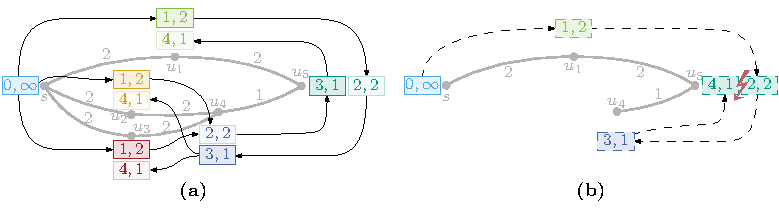
\includegraphics{switchplacement/figures/dtp_labels_to_colored_dag.pdf}
    %
    \caption[The directed label graph after an {\gls{dtp}}-algorithm
    execution.]{%
    A network~\glssymbol{network} and the corresponding directed graph on
    the labels computed during the execution of the {\gls{dtp}}-algorithm.
    All edges~$(\vertexa,\vertexb)\in\glssymbol{edges}$ have
    susceptance~$\textcolor{SUSCEPTANCE}{\glssymbol{susceptance}\equiv 1}$.
    Two labels have the same color if and only if they belong to the same
    vertex in~\glssymbol{network}. (a) To test whether the label~$(4,1)$
    at~$\vertexa_3$ shall be inserted into the graph, we search for a
    rainbow path from the label at~\source to the new label~$(4,1)$. The
    slightly colored labels produce no~\gls{dtp} from that particular
    vertex. (b) The rainbow path avoids cycles and ensures that the paths
    remain simple. 
    }%
    % 
    \label{ch:switching:sec:exploit_structural_characteristics:fig:dtp_labels_to_colored_dag}
\end{figure}
% 
A counterexample for monotone voltage angle paths is given in~\cref{ch:switching:sec:exploit_structural_characteristics:fig:labels_and_does_not_lie_on_monoton_theta_paths} 
confirming~\cref{ch:switching:sec:exploit_structural_characteristics:lem:dtp-monotony}.
%
\begin{lemma}
    The~\acrlong{dtp} (\gls{dtp}) is not necessarily on a monotone voltage
    angle path.
    % 
    \label{ch:switching:sec:exploit_structural_characteristics:lem:dtp-monotony}
\end{lemma}  
% 
%%%%%%%%%%%%%%%%%%%%%%%%%%%%%%%%%%%%%%%%%%%%%%%%%%%%%%%%%%%%%%%%%%%%%%%%%%%%%%%%
\subsection{DTP without Merging the Labels}
\label{ch:switching:sec:exploit_structural_characteristics:subsec:DTP_without_label_merging}
%%%%%%%%%%%%%%%%%%%%%%%%%%%%%%%%%%%%%%%%%%%%%%%%%%%%%%%%%%%%%%%%%%%%%%%%%%%%%%%%
% 
The~\cref{ch:switching:sec:exploit_structural_characteristics:subsec:dtp:alg:shortest_theta_path}
for the~\gls{dtp} can be implemented using the merging of equivalent labels or
without merging. Neglecting the merging of labels would mean that we
remove~\cref{ch:switching:sec:exploit_structural_characteristics:subsec:dtp:alg:shortest_theta_path:line:check_reachability}
that avoids cycles
and~\cref{ch:switching:sec:exploit_structural_characteristics:subsec:dtp:alg:shortest_theta_path:line:check}
that merges the labels. Thus, the reachability check is neglected, but we have
to add cycle checks that are also done by the reachability test
(see~\cref{ch:switching:sec:exploit_structural_characteristics:subsec:reachibility_test}).
The implementation stores a set of visited vertices~$\glssymbol{vertices}'$ for
every label. Using a simple union operation on these set, we are able to check
for cycles. In worst-case we have to
save~$\bigO(\fmagnitude{\glssymbol{vertices}})$ elements per vertex in that set.
Thus, a label consists in that case of~$(\bnorm{\cdot}, \glssymbol{mincapacity}
(\cdot),\glssymbol{vertices}')$. Note that this method can lead to exponential
many labels as exemplified
in~\cref{ch:switching:sec:exploit_structural_characteristics:subsec:dtp:fig:non_poly_number_of_labels}.
However, the reachability test leads to an exponential running time
(see~\cref{ch:switching:sec:exploit_structural_characteristics:subsec:reachibility_test,ch:switching:sec:exploit_structural_characteristics:eq:runtime_exp_DTP}).% %%%%%%%%%%%%%%%%%%%%%%%%%%%%%%%%%%%%%%%%%%%%%%%%%%%%%%%%%%%%%%%%%%%%%%%%%%%%%%%%
\subsection{Reachability Test}
\label{ch:switching:sec:exploit_structural_characteristics:subsec:reachibility_test}
%%%%%%%%%%%%%%%%%%%%%%%%%%%%%%%%%%%%%%%%%%%%%%%%%%%%%%%%%%%%%%%%%%%%%%%%%%%%%%%%
% 
\cref{ch:switching:sec:exploit_structural_characteristics:subsec:dtp:alg:shortest_theta_path}
repeatedly tests whether the new labels correspond to simple paths in the
network
(\cref{ch:switching:sec:exploit_structural_characteristics:subsec:dtp:alg:shortest_theta_path:line:check_reachability}
of
\cref{ch:switching:sec:exploit_structural_characteristics:subsec:dtp:alg:shortest_theta_path}).
For this it is checked whether the label at vertex~\source is reachable
from~\vertexa via
\parent-pointers from the label~\glssymbol{label} when all labels at~\vertexb
are ignored. The labels and the pointers together form a directed acyclic graph,
where the labels have the same color if and only if they belong to the same
vertex in network~\glssymbol{network}
(see~\cref{ch:switching:sec:exploit_structural_characteristics:fig:dtp_labels_to_colored_dag}).
We call a path whose vertices all have different colors a \emph{rainbow path}.
%
%%%%%%%%%%%%%%%%%%%%%%%%%%%%%%%%%%%% FIGURE %%%%%%%%%%%%%%%%%%%%%%%%%%%%%%%%%%%%
\begin{figure}[t!]
  \centering
  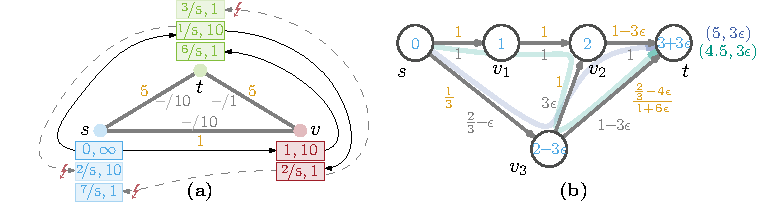
\includegraphics{switchplacement/figures/labels_and_does_not_lie_on_monoton_theta_paths.pdf}
  %
  \caption[\gls{dtp} problematic cases.]{%
  The graphs represent two problematic cases. (a) An example that shows that it
  does not suffice that the labels consist
  of~$(\bnorm{\cdot},\glssymbol{mincapacity}(\cdot))$, but has to include the
  set of visited vertices~$\glssymbol{vertices}'$. (b) Shows an example that
  the~\gls{dtp} is not necessarily on a monotone voltage angle path. Let~$0 <
  \epsilon \ll \nicefrac{2}{3}$ then the green path represents the~\gls{dtp}
  from~\source to~\sink. }%
  % 
  \label{ch:switching:sec:exploit_structural_characteristics:fig:labels_and_does_not_lie_on_monoton_theta_paths}
\end{figure}
%
\begingroup
    %%%%%%%%%%%%%%%%%%%%%%%%%%%%%%%%%%% Problem %%%%%%%%%%%%%%%%%%%%%%%%%%%%%%%%%%%%
\begin{problem}[framed]{\acrlong{strp}~$\gls{strp}(
\glssymbol{graph},c,\source,\sink)$}
    Instance: & A directed acyclic graph~$\glssymbol{graph} =
    (\glssymbol{vertices},\glssymbol{edges})$, a
    coloring~$\col\colon\glssymbol{vertices}\to\naturals$, and $\source,
    \target\in\glssymbol{vertices}$.\\
    % 
    Question: & Is there an~\source-\target-path~$\pathu$ in~\glssymbol{graph}
    such that all vertices of~$\pathu$ have different colors?
\end{problem} 
    \label{ch:switching:problems:Rainbow_s_t_path-Decision_Problem}
\endgroup
%
An algorithm to test whether there is a~\acrlong{strp} (\gls{strp}) in
undirected graphs was presented by~\textcite[Theorem~11]{Uch13}. It runs
in~$\bigO(k2^k \fmagnitude{\glssymbol{edges}}\fmagnitude{\glssymbol{vertices}})$
time, where~$k$ is the number of colors, $\fmagnitude{\glssymbol{edges}}$ the
number of edges, and~$\fmagnitude{\glssymbol{vertices}}$ the number of vertices
in~\glssymbol{graph}. We give a different algorithm for directed graphs, which
can be implemented to run in~$\bigO(k2^k\fmagnitude{\glssymbol{edges}})$ time.
The main work is done
by~\cref{ch:switching:sec:exploit_structural_characteristics:alg:compute_colors}.
It additionally gets a set~$\forbidden$ of forbidden colors as input and ignores
all vertices of these colors. To decide whether there is a rainbow path from a
vertex~\source to a vertex~\target, we initially set~\forbidden to~$\emptyset$.
We compute for each vertex~\vertex a set of
colors~$\colorlabels_\forbidden(\vertex)$. A color~\col is in the
set~$\colorlabels_\forbidden(\vertex)$ if and only if any
rainbow~\source-\vertex-path~$\fpath{}{\source}{\vertex}$ contains a vertex with
color~\col with the additional constraint that no vertex of~$\fpath{}{\source}
{\vertex}$ is colored with a color in~$\forbidden$
(in~\cref{ch:switching:sec:exploit_structural_characteristics:alg:compute_colors}~\cref{ch:switching:sec:exploit_structural_characteristics:alg:compute_colors:5,ch:switching:sec:exploit_structural_characteristics:alg:compute_colors:6}).
For each vertex~\vertexb and all its incoming edges~$(\vertexa,\vertexb)$ we
recursively compute all necessary colors for the rainbow paths to $\vertexa$
such that~$\col(\vertexb)$ is forbidden. The
set~$\colorlabels_\forbidden(\vertexb)$ is then equal to the intersection of
these color sets together with~$\col(\vertexb)$. Throughout the algorithm we
use~$\naturals$ to indicate that there is no rainbow path with the given
restrictions.

During the
execution~\cref{ch:switching:sec:exploit_structural_characteristics:alg:compute_colors}
may be called several times with the same parameters. To speed up the
computation one may store the results instead of recomputing them every time.
Further, we find a relation between~$\colorlabels_\forbidden(\vertex)$
and~$\colorlabels_{\forbidden'}(\vertex)$ for a vertex~\vertex and two sets of
forbidden colors~\forbidden and~$\forbidden'$. If every color of a vertex
before~\vertex in the topological order is either both in~\forbidden
and~$\forbidden'$ or neither in~\forbidden nor~$\forbidden'$, we
have~$\colorlabels_\forbidden(\vertex) =
\colorlabels_{\forbidden'}(\vertex)$. In particular, if no vertex
before~$\vertex$ is colored by any color in~$\forbidden$, we
have~$\colorlabels_\forbidden(\vertex)=\colorlabels_\emptyset(\vertex)$. This
property can also be used to reduce the number of recursive calls.

Alternatively, the set of colors~$\colorlabels_\forbidden(\vertex)$ at a
vertex~\vertex can be computed by traversing all paths from~\source to~\vertex,
checking if no two vertices are colored the same and finally taking the common
colors of all rainbow paths. This may be faster if there are only
few~\source-\vertex-paths or if many of the paths can be eliminated quickly
because they are not rainbow paths.
% 
%%%%%%%%%%%%%%%%%%%%%%%%%%%%%%%%%% ALGORITHM %%%%%%%%%%%%%%%%%%%%%%%%%%%%%%%%%%%
\begin{algorithm}[tb!]
    \SetAlgoLined
    % 
    \KwData{%
        A directed label network~$\coloredgraph=(\glssymbol{graph}=
        (\glssymbol{vertices},\glssymbol{edges}),\col, \source)$,
        where~$\col\colon\glssymbol{vertices}\to\naturals$ is the coloring
        and~$\source\in\glssymbol{vertices}$ is the fixed source of the network,
        $\vertexb\in\glssymbol{vertices}$, and a
        set~$\forbidden\subseteq\naturals$ of forbidden colors. }
    % 
    \KwResult{%
        The intersection of the colors of all rainbow 
        \source-\vertexb-paths, or~$\naturals$ if there are no such paths. }

    \lIf(\Comment*[f]{\color{KITblack30}Not a rainbow path?})
        {$\col(\vertexb)\in\forbidden$}%
    {%
        \Return{\naturals}
        \label{ch:switching:sec:exploit_structural_characteristics:alg:compute_colors:1}
    } % if
    \lIf(\Comment*[f]{\color{KITblack30}Base case})
        {$\source=\vertexb$}%
    {%
        \Return{$\{\col(\source)\}$}%
        \label{ch:switching:sec:exploit_structural_characteristics:alg:compute_colors:2}
    } % if
    $\colorlabels_\forbidden(\vertexb) \coloneq \naturals$\;
    \label{ch:switching:sec:exploit_structural_characteristics:alg:compute_colors:3}
    %  
    \For(\Comment*[f]{\color{KITblack30}All incoming edges into~\vertexb}){
        $(\vertexa,\vertexb)\in\edges$
    }{
        $C'\coloneqq\computeColors\left(\coloredgraph, \vertexa, 
        \forbidden\cup\{\col(\vertexb)\}\right)$\Comment*
        {\color{KITblack30}Incoming cut}
        \label{ch:switching:sec:exploit_structural_characteristics:alg:compute_colors:5}
        % 
        $\colorlabels_\forbidden(\vertexb) \coloneqq 
        \colorlabels_\forbidden(\vertexb) \cap C'$\;
        \label{ch:switching:sec:exploit_structural_characteristics:alg:compute_colors:6}
    } % for
    $\colorlabels_\forbidden(\vertexb) \coloneqq \colorlabels_\forbidden
    (\vertexb) \cup \{\col(\vertexb)\}$\;
    \label{ch:switching:sec:exploit_structural_characteristics:alg:compute_colors:8}
    % 
    \Return{$\colorlabels_\forbidden(\vertexb)$}\;
    \label{ch:switching:sec:exploit_structural_characteristics:alg:compute_colors:9}
    % 
    \caption{computeColors}
    % 
    \label{ch:switching:sec:exploit_structural_characteristics:alg:compute_colors}
\end{algorithm}
% 
%%%%%%%%%%%%%%%%%%%%%%%%%%%%%%%%%%%%%%%%%%%%%%%%%%%%%%%%%%%%%%%%%%%%%%%%%%%%%%%%
%%%%%%%%%%%%%%%%%%%%%%%%%%%%%%%%%%%%%%%%%%%%%%%%%%%%%%%%%%%%%%%%%%%%%%%%%%%%%%%%
\subsection{Analyses of the DTP}
\label{ch:switching:sec:exploit_structural_characteristics:subsec:dtp_analyses}
%%%%%%%%%%%%%%%%%%%%%%%%%%%%%%%%%%%%%%%%%%%%%%%%%%%%%%%%%%%%%%%%%%%%%%%%%%%%%%%%
% 
Examples of this algorithm are shown 
% 
in the upper part of~\cref{fig:comparing_delta_theta_path}\screen{a}
and~\screen{b}. Note that there are at most~$\fmagnitude{\glssymbol{edges}}$
different values of~$\glssymbol{mincapacity}(\cdot)$
since there are at most~$\fmagnitude{\glssymbol{edges}}$ different labels saved per vertex
assuming that we merge and have a penrose-minor free graph with direction. This
bound is tight. Consider for example two vertices with~$\fmagnitude{\glssymbol{edges}}$
parallel lines, where line~$i$ has capacity~$i$ and
susceptance~$\nicefrac{1}{i}$.
%
\begin{lemma}
  For each~$\vertexa\in\glssymbol{vertices}$ we have~$\fmagnitude{
    \glssymbol{labels}(\vertexa)}\le\fmagnitude{\glssymbol{edges}}$.
  \label{ch:switching:sec:exploit_structural_characteristics:lem:label_set_bound}
\end{lemma}
%
Note that for arbitrary graphs the labels are of the form~$(\bnorm{\cdot},
\glssymbol{mincapacity}(\cdot),\glssymbol{vertices}')$, which results in
exponential many
labels. The non-negativity of the susceptance norm and capacity implies that
processed labels~$\glssymbol{paretolabels}(\cdot)$ will not be removed. This is
denoted as \emph{label setting}. In contrast, negativity would imply that there
may exist a path such that processed labels have to be updated by labels of
vertices on the negative path. In addition, all adjacent labels of the updated
labels have to be corrected and so forth. Algorithms working like this are
called \emph{label correcting} and do not perform as efficiently as label
setting algorithms.
% 
The running time
of~\cref{ch:switching:sec:exploit_structural_characteristics:subsec:dtp:alg:shortest_theta_path}
depends on the subroutine \texttt{isReachable} for which no polynomial bound is
known. Note that these tests are easy for labels that correspond to exactly one
path, \ie, labels that were not merged. On realistic power grid instances the
algorithm performs well since merging is rare.
% 
If we use a Fibonacci-heap~\glssymbol{priorityqueue} to store labels, the
operation~\myinsert is in~$\bigO(1)$, \deleteMin is amortized in~$\bigO(\log
\fmagnitude{\glssymbol{vertices}})$~\parencite{715934}, \deleteDominatedLabels is
in~$\bigO(\fmagnitude{\glssymbol{edges}})$, and~\isReachable
(see~\cref{ch:switching:sec:exploit_structural_characteristics:subsec:reachibility_test})
runs in~$\bigO (2^{\fmagnitude{\glssymbol{vertices}}} 
\fmagnitude{\glssymbol{vertices}}\cdot\fmagnitude{\glssymbol{edges}})$
time. The initialization is in~$\bigO(\fmagnitude{\glssymbol{vertices}})$ time
(\crefrange{alg:initialization_begin}{alg:initialization_end}). There
are~$\bigO(\fmagnitude{\glssymbol{vertices}}\cdot\fmagnitude{\glssymbol{edges}})$
\deleteMin operation, since every vertex can have up
to~$\fmagnitude{\glssymbol{edges}}$ labels. There
arise~$\bigO(\fmagnitude{\glssymbol{edges}}^2)$ operations of all other methods, since we
do these operation for all incident
edges~$\sum_{\vertexa\in\glssymbol{vertices}}
\deg(\vertexa) = 2\fmagnitude{\glssymbol{edges}}$~\parencite{Eul36}
(\cref{alg:check_adjacent_vertices}) and each vertex can have at
most~$\fmagnitude{\glssymbol{edges}}$ labels. Thus, the algorithm runs in time% 
% 
% 
\begin{align}
T\coloneq&\,\bigO\big(\fmagnitude{\glssymbol{vertices}}\cdot
\fmagnitude{\glssymbol{edges}}\cdot
T_{\deleteMin}
  + \fmagnitude{\glssymbol{edges}}^2\cdot \notag\\ &\left( T_{\myinsert} + T_{\isReachable}
    + T_{\deleteDominatedLabels} \right)
\big)\\
% 
=&\,\bigO\left(\fmagnitude{\glssymbol{vertices}}\cdot\fmagnitude{\glssymbol{edges}}\cdot
\log \fmagnitude{\glssymbol{vertices}} +
  2^{\fmagnitude{\glssymbol{vertices}}}\fmagnitude{
  \glssymbol{vertices}}\cdot\fmagnitude{\glssymbol{edges}}^3\right).
  % 
  \label{ch:switching:sec:exploit_structural_characteristics:eq:runtime_exp_DTP}
  %
%
\end{align}
% 
The following lemma results directly from the previous discussion.
% 
\begin{lemma}
  
\cref{ch:switching:sec:exploit_structural_characteristics:subsec:dtp:alg:shortest_theta_path}
runs in~$\bigO\left(2^{\fmagnitude{\glssymbol{vertices}}}\fmagnitude{\glssymbol{vertices}}\cdot\fmagnitude{\glssymbol{edges}}^3\right)$ time.
\end{lemma}
% 
% 
On general graphs we cannot assume that the switched edges are either tight
edges (\ie, bottleneck edges that are congested) or on the~\gls{dtp}
(in~\cref{fig:comparing_delta_theta_path}\screen{b} edge~$(\vertexa,\vertexb)$
is not on the~\gls{dtp}).
% 
%
In the following, we restrict our graph classes of the
network~\glssymbol{network} to~\source-\sink-networks (\ie, there is only
one~$\source\in\glssymbol{generators}$ and one~$\sink\in\glssymbol{consumers}$)
and try to solve the~\gls{mtsfp} on them. We identify structures, where
it is easy to switch. The following lemma shows at which point it is beneficial
to switch on simple cycles.
%
%%%%%%%%%%%%%%%%%%%%%%%%%%%%%%%%%%%% LEMMA %%%%%%%%%%%%%%%%%%%%%%%%%%%%%%%%%%%%
\begin{lemma}
  Let~\glssymbol{network} be a simple cycle with one generator~\source and one
  consumer~\sink, and let~$
  \fpath{}{\source}{\sink}\in\paths(\source,\sink)\setminus\fpath{\gls{dtp}}
  {\source}{\sink}$. The Braess's Paradox exists if and only
  if~$~\opt_{\gls{mpfp}}(\fpath{}{\source}{\sink})$ $>
  \opt_{\gls{mpfp}}(\glssymbol{network})$.
  % 
  \label{ch:switching:sec:exploit_structural_characteristics:lem:braess-paradox-path-cycle}
\end{lemma}
%  
%
\begin{proof}
%
It suffices to show that removing
edge~$\edge_{\min}(\fpath{\gls{dtp}}{\source}{\sink})\coloneqq
\argmin_{\edge\in\fpath{\gls{dtp}}{\source}{\sink}}\capacity(\edge)$ results
in~$\opt_{\gls{mpfp}}(\glssymbol{network}-\{\edge_{\min}\}) > \opt_{
\gls{mpfp}} (\glssymbol{network})$ and thus,
it holds~$\opt_{\gls{mtsfp}}(\glssymbol{network}) > \opt_{\gls{mpfp}}(
\glssymbol{network})$.
% 
The flow on the path~$\fpath{}{\source}{\sink}$ is defined by the
ratio~$\nicefrac{
\glssymbol{voltageangledifference}(\fpath{}{\source}{\sink})}{\bnorm{\fpath{}{\source}{\sink}}
}$ (\cref{ch:switching:sec:model:eq:KVL_dc_approx,eq:bnorm}). 
% 
The smallest voltage angle difference~$\glssymbol{voltageangledifferencemin}(\source,\sink)$
restricts the flow on the other path~$
\fpath{}{\source}{\sink}$. Thus, the term~$\nicefrac{
\glssymbol{voltageangledifferencemin}(\source,\sink)}{\bnorm{\fpath{}{\source}{\sink}}
}$ is the maximum possible flow on path~$\fpath{}{\source}{\sink}$.
%
% 
The value $\opt_{\gls{mpfp}}(\fpath{}{\source}
{\sink}) > \opt_{\gls{mpfp}}(\glssymbol{network})$ holds if and only if
% 
\begin{align*}
\frac{\glssymbol{voltageangledifference}(\fpath{}{\source}{\sink})}{\bnorm{\fpath{}{\source}{\sink}}} 
%
& >
%
\glssymbol{voltageangledifferencemin}(\source,\sink)
\cdot
\frac{\bnorm{\fpath{}{\source}{\sink}}
+ 
\bnorm{\fpath{\gls{dtp}}{\source}{\sink}}}
%
{\bnorm{\fpath{}{\source}{\sink}}
\cdot\bnorm{\fpath{\gls{dtp}}{\source}{\sink}}}.
%
% 
\end{align*}
Thus, switching an edge~$\edge_{\min}$
on~$\fpath{\gls{dtp}}{\source}{\sink}$
increases the total flow on the cycle and makes switching beneficial.
\end{proof}
% 
% 
We now generalize this result to a more complex graph class. Following the
construction in~\cref{ch:switching:sec:network_modeling}, we assume that all
generator and consumer vertices have degree~$1$. A diamond graph is a simple
graph on four vertices and five edges consisting of two triangle facets
identified along an edge. Moreover, we denote its degree-$3$ vertices as
\emph{girdle} vertices and its degree-2 vertices as its \emph{tip} vertices.
Furthermore, we call the combination of a \emph{kite} and a \emph{dart} graph
representing both diamond graphs with an additional edge on one of the tip and
the girdle vertices, respectively, a \emph{penrose} graph
(\cref{ch:switching:sec:exploit_structural_characteristics:fig:forbidden_minor}).
These additional edges basically represent either a generator edge or a consumer
edge, but not both the same. We emphasize this by the following definition.
% 
%%%%%%%%%%%%%%%%%%%%%%%%%%%%%%%%%%%% FIGURE %%%%%%%%%%%%%%%%%%%%%%%%%%%%%%%%%%%%
\begin{figure}[t!]
  \centering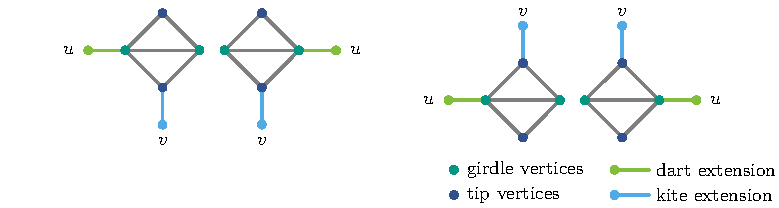
\includegraphics{switchplacement/figures/forbidden_minor.pdf}
  %
  \caption[A description of penrose-minors.]{All cases show penrose-minors,
  where~\vertexa and~\vertexb are either generators or consumers, but not both
  the same. They are a combination of a \screentextcolor{KITcyanblue}{kite
  graph} (\ie, diamond graph with an additional edge on one of the
  \screentextcolor{KITseablue}{tip vertices}) and
  a~\screentextcolor{KITpalegreen}{dart graph} (\ie, diamond graph with an
  additional edge on one of the
  \screentextcolor{KITgreen}{girdle vertices}).  
  }%
  \label{ch:switching:sec:exploit_structural_characteristics:fig:forbidden_minor}
\end{figure}
% 
\begin{definition}[Penrose Graph]
    A \emph{penrose} graph is a kite graph with an additional edge incident to
    one of the girdle vertices, or similarly, a dart graph with an additional
    edge on one of the tip vertices.
    % 
    \label{ch:switching:sec:exploit_structural_characteristics:def:penrose-graph}
\end{definition}
% 
A \emph{minor} of a network~\glssymbol{network} is obtained
from~\glssymbol{network} by contracting and deleting edges, as well as deleting
isolated vertices (\ie, vertices without incident edges).
% 
A~\emph{penrose-minor-free graph} is a graph 
% 
without a penrose graph as a minor.
%

In the following, we consider penrose-minor-free graphs with one
generator~\source and one consumer~\sink. Note that each block, \ie, a maximal
biconnected subgraph, of such graphs consist of one or more parallel paths. The
start and end vertices of the paths act as generator and consumer for the block.
Note that the blocks can be considered separately. Let~\block be a block
and~\vertexa and~\vertexc the start and end vertices of its paths. The flow
value~\glssymbol{flowvalue} of an~\gls{mpf} from~\vertexa to~\vertexc is
%
%%%%%%%%%%%%%%%%%%%%%%%%%%%%%%%%%%% EQUATION %%%%%%%%%%%%%%%%%%%%%%%%%%%%%%%%%%%
% 
$
% 
%
%
\glssymbol{flowvalue} = 
%%%%%%%
\glssymbol{voltageangledifferencemin}(\vertexa, \vertexc)
%
\cdot
%
\sum_{\pathu\in\glssymbol{pathset}(\vertexa,\vertexc)} 
\frac{1}{\bnorm{\pathu}}.%
%
$
%
To increase the flow value, either of the factors has to be increased. Switching
cannot increase the sum, but only the angle difference on the~\gls{dtp}. Thus,
the following result holds.
% 
\begin{lemma}
    Switching on~penrose-minor-free graphs is only beneficial
    on~\gls{dtp}{s}.
    % 
    \label{ch:switching:sec:exploit_structural_characteristics:lem:switching_in_DTP}
\end{lemma}
% 
From~\cref{ch:switching:sec:exploit_structural_characteristics:lem:switching_in_DTP}
we know that we only need to consider edges on a~\gls{dtp} for switching.
In~\cref{ch:switching:sec:exploit_structural_characteristics:alg:msf_series_parallel_structures}
for each block~\block\ we remove the edge with the smallest capacity
on~$\fpath{\gls{dtp}}{\source}{\sink}$ in~\block and update
the~$\gls{dtp}(\source,\sink)$. If we get a better value
for~\glssymbol{flowvalue}, we save it. We repeat this procedure until there is
no path from~\source to~\sink.
% 
The correctness of~\cref{ch:switching:sec:exploit_structural_characteristics:alg:msf_series_parallel_structures} follows directly 
from the correctness of the~\gls{dtp}-Algorithm 
(\cref{ch:switching:sec:exploit_structural_characteristics:subsec:dtp:alg:shortest_theta_path}) and~\cref{ch:switching:sec:exploit_structural_characteristics:lem:switching_in_DTP}.
% 
\begin{theorem}
  
\cref{ch:switching:sec:exploit_structural_characteristics:alg:msf_series_parallel_structures}
  computes a correct~\gls{mtsf} on penrose-minor-free graphs with one generator
  and one consumer.
  % 
  \label{ch:switching:sec:exploit_structural_characteristics:lem:algo2_correct_msf_on_st_diamond_graphs}
\end{theorem}
%
% 
%%%%%%%%%%%%%%%%%%%%%%%%%%%%%%%%%% ALGORITHM %%%%%%%%%%%%%%%%%%%%%%%%%%%%%%%%%%%
\wormhole{bit:ch:switching:sec:exploit_structural_characteristics:alg:msf_series_parallel_structures}
\def\HiLi{\leavevmode\rlap{\hbox to \hsize{\color{KITyellow15}\leaders\hrule
height .9\baselineskip depth 1.5ex\hfill}}}
\begin{algorithm}[tb!]%
\SetAlgoLined
  % 
  \SetKwFunction{blockCutTree}{blockCutTree}
  % 
  \KwData{A network~$\glssymbol{network} = 
  (\glssymbol{graph},\glssymbol{generators},\glssymbol{consumers},\glssymbol{capacity},\glssymbol{susceptance})$.}
  % 
  \KwResult{$\dtp(\source,t)$,
  $\parent\colon\glssymbol{vertices}\to\glssymbol{vertices}$, and
  $\lab\colon\glssymbol{vertices}\!\to\posreals\times\posreals$.}
  % 
  % INITIALIZATION %%%%%%%%%%%%%%%%%%%%%%%%%%%%%%%%%%%%%%%%%%%%%%%%%%%%%%%%%%%%
  $\glssymbol{switched} \coloneqq \emptyset$\;
  $\blocks\ \coloneqq \blockCutTree(\glssymbol{network})$
  \Comment*{\color{KITblack30}Biconnected components}
  $(\pathu_{\glssymbol{dtp}}, \deltaangle_{\min}, \parent, \glssymbol{labels}(\cdot)) \coloneqq \dtp
  (\glssymbol{network})$\Comment*
  {
  \color{KITblack30}see {\hypersetup{linkcolor=KITblack30}
  \cref{ch:switching:sec:exploit_structural_characteristics:subsec:dtp:alg:shortest_theta_path}}}
  \For{$\block\in\blocks$}
  {
    $\glssymbol{switched}' \coloneqq \emptyset$\;
    \While{$\glssymbol{labels}(\sink)\ne\emptyset$}
    {
      %
      $\glssymbol{switched}' 
      \coloneqq 
      \glssymbol{switched}'
      \cup
      \edge_{\min}(\fpath{\glssymbol{dtp}}{\source}{\sink})$\;
      % 
      \If
      {$\opt_{\gls{mpfp}}(\block-\glssymbol{switched}')\geq\opt_{\gls{mpfp}}
      (\block-
      \glssymbol{switched})$}
      {
        $\glssymbol{switched} \coloneqq \glssymbol{switched} \cup 
        \glssymbol{switched}'$\Comment*{\color{KITblack30}Save switched
        lines in~\glssymbol{switched}}
      }
      $(\pathu_{\dtp}, \glssymbol{voltageangledifference}_{\min}, \parent, \lab)
      \coloneqq
      \dtp
      (\block-\glssymbol{switched}')$\Comment*{
      \color{KITblack30}Update}
    }
  }%for  
  \Return{$\left(\opt_{\gls{mpfp}}(\glssymbol{network}-\glssymbol{switched}),\glssymbol{switched}\right)$}\;
  \caption{\gls{mtsf}\ Algorithm for Penrose-Minor-Free~\glssymbol{network}}%
  \label{ch:switching:sec:exploit_structural_characteristics:alg:msf_series_parallel_structures}%
\end{algorithm}%
%
Switching is~\NP-hard in series-parallel graphs, which generalize
penrose-minor graphs, and leads to the next lemma that was proven in~\cref{ch:switching:sec:complexity:subsec:np_hardness_Source_Sink_MTSF_capacity1}.
% 
\begin{lemma}
    \gls{mtsfp} is~\NP-hard even if there is only one source and one sink in
    the network and all edge capacities are~$1$.
\end{lemma}

A general observation in power grids is that shortest paths are somehow
connected to switching a line, since the betweenness centrality is negatively
correlated to switching lines~\parencite{4438889}.
% 
Though switched edges on general graphs are not always on~\gls{dtp}{s},
\cref{ch:switching:sec:exploit_structural_characteristics:subsec:dtp:alg:shortest_theta_path} gives us a new criterion focusing on switching by
using~\gls{dtp}{s} instead of the shortest paths. We define
the~\gls{dtp} centrality based on the number of~\gls{dtp}{s} through
an edge.
% 
\begin{definition}
% 
    Let~\glssymbol{network} be a power grid. The~\gls{dtp} betweenness
    centrality~$c_{\sbc}\colon\glssymbol{edges}\to\posreals$ is defined by
    \begin{equation}
        c_{\sbc}(\edge) \coloneqq 
        \frac{1}{m_B}\sum_{\source\in\glssymbol{vertices}}
        \sum_{\sink\in\glssymbol{vertices}\setminus\{\source\}}
        \frac{\sigma_{\gls{dtp}}(\source, \sink, \edge)}{\sigma_{\gls{dtp}}(\source,
        \sink)},
    \end{equation}
    where~$\sigma_{\gls{dtp}}(\source, \sink, \edge)$ is the number
    of~\gls{dtp}{s} between~\source and~\sink that use~\edge,
    $\sigma_{\gls{dtp}}(\source,
    \sink)$ is the total number of~\gls{dtp}{s} from~\source to~\sink 
    and~$m_B = \fmagnitude{\glssymbol{vertices}}
    (\fmagnitude{\glssymbol{vertices}} - 1)$ is a normalizing constant.
    % 
    \label{ch:switching:sec:exploit_structural_characteristics:def:dtp_betweenness_centrality}
    % 
\end{definition}
% 
% 
For directed and undirected graphs, the normalization factor is the same, since
the algorithm operates on the directed label graph. However, we normalize the
number of~\gls{dtp}{s} already by the number of~\gls{dtp}{s} between~\source
and~\sink. Note that in power grids we do not necessarily check all pairs of
vertices, but the paths between all
generators~$\source\in\glssymbol{generators}$ and
consumers~$\sink\in\glssymbol{consumers}$. Thus, we define the following
centrality that differs in the base---meaning generators and consumers instead
of all vertices---and normalization constant.
% 
\begin{definition}%
    % 
    Let~\glssymbol{network} be a power grid. The switching
    centrality~$c_{\scu}\colon\glssymbol{edges}\to\posreals$ is defined by%
    \begin{equation}%
        c_{\scu}(\edge) \coloneqq
        \frac{1}{m_B}\sum_{\source\in\glssymbol{generators}}
        \sum_{\sink\in\glssymbol{consumers}}
        \frac{\sigma_{\gls{dtp}}(\source, \sink,
        \edge)}{\sigma_{\gls{dtp}}
        (\source,
     \sink)},%
    \end{equation}%
    where~$\sigma_{\gls{dtp}}(\source, \sink, \edge)$ is the number
    of~\gls{dtp}-paths between~\source and~\sink that use edge~\edge,
    $\sigma_{\gls{dtp}}(\source, \sink)$ is the total number of~\gls{dtp}-paths
    from~\source to~\sink
    and~$m_B=\fmagnitude{\glssymbol{generators}}\cdot\fmagnitude{\glssymbol{consumers}}$
    is a normalizing constant.%
    % 
    \label{ch:switching:sec:exploit_structural_characteristics:def:s_t_dtp_betweenness_centrality}%
    % 
\end{definition}%
% 
% 
%%%%%%%%%%%%%%%%%%%%%%%%%%%%%%%%%%%%%%%%%%%%%%%%%%%%%%%%%%%%%%%%%%%%%%%%%%%%%%%%
%%%%%%%%%%%%%%%%%%%%%%%%%%%%%%%%%%%%%%%%%%%%%%%%%%%%%%%%%%%%%%%%%%%%%%%%%%%%%%%%
\section{Computing one DTP in Polynomial Time}
\label{ch:switching:sec:computing_one_dtp}
%%%%%%%%%%%%%%%%%%%%%%%%%%%%%%%%%%%%%%%%%%%%%%%%%%%%%%%%%%%%%%%%%%%%%%%%%%%%%%%%
% 
\begin{figure}[t!]
    % 
    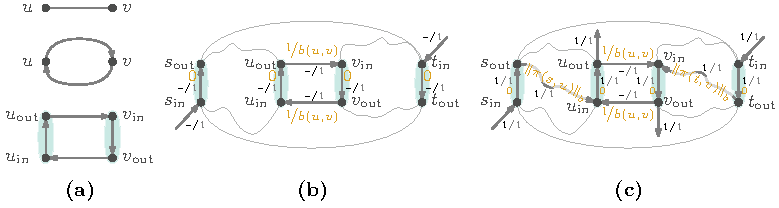
\includegraphics{switchplacement/figures/polynomial_dtp_direct_edges.pdf}
    % 
    \caption[Necessary graph transformation to calculate a polynomial algorithm.]
    {The necessary graph transformations to calculate a~\gls{dtp} in polynomial
    time. (a) The transformation from an undirected graph to a directed graph
    that is bidirected by transforming edge~$\{\vertexa,\vertexb\}$ to two
    directed edges~$(\vertexa,\vertexb), (\vertexb,\vertexa)$. To have a vertex
    disjoint path, each vertex~\vertexa is split into two
    vertices~$\vertexa_{\mathrm{in}},\vertexa_{\mathrm{out}}$ with one
    additional edge~$(\vertexa_{\mathrm{in}},\vertexa_{\mathrm{out}})$. (b) The
    transformed network~$\glssymbol{network}''$ with
    capacities~$\glssymbol{capacity}\equiv 1$ and edges
    costs~$\gamma(\vertexa_{\mathrm{out}},\vertexb_{\mathrm{in}}) =
    \nicefrac{1}{\glssymbol{susceptance}(\vertexa_{\mathrm{out}},\vertexb_{
    \mathrm{in}})}$ for an external edge
    and~$\gamma(\vertexa_{\mathrm{in}},\vertexa_{\mathrm{out}}) = 0$ for a
    vertex internal edge. (c) The resulting minimum-cost flow~\glssymbol{flow}
    for an edge~$\edge_{\min} = (\vertexa,\vertexb)$. }%
    % 
    \label{ch:switching:sec:computing_one_dtp:fig:poly-alg}
    % 
\end{figure}
% 
The previous algorithm computes all~\gls{dtp}{s} between two vertices~\vertexa
and~\vertexb, but has an exponential running time or uses exponential space
dependent on the implementation. In this section, we present a polynomial time
algorithm to calculate the~\gls{dtp}. However, instead of calculating
all~\gls{dtp}{s} between two vertices~\vertexa and~\vertexb this algorithm
computes only one~\gls{dtp}. Thus, it cannot be used for the centrality
measurement. Recall
from~\cref{ch:switching:sec:exploit_structural_characteristics:subsec:dtp} that
a label~$(\bnorm{\fpath{}{\source}{\vertexa}},
\glssymbol{mincapacity}(\fpath{}{\source}{\vertexa}))$ consists of the
susceptance norm---representing the electrical distance---and the minimum
capacity along a path~$\fpath{}{\source}{\vertexa}$. Thus, fixing the edge with
the smallest capacity and calculating a shortest path from that particular edge
to the source and sink vertex using the susceptance norm~$\bnorm{\cdot}$ is
equivalent to the bicriterial shortest path.
% 
%%%%%%%%%%%%%%%%%%%%%%%%%%%%%%%%%% ALGORITHM %%%%%%%%%%%%%%%%%%%%%%%%%%%%%%%%%%%
% \begin{algorithm}[tb!]
%   \SetAlgoLined
%   \SetKwFunction{kwfTodo}{todo}
%   \SetKwFunction{isMarked}{isMarked}
%   \SetKwFunction{kwfUnmark}{unmark}
%   \SetKwFunction{kwfMark}{mark}
%   \SetKwFunction{kwfPush}{push\_back}
%   \SetKwFunction{kwfParent}{parent}
%   \SetKwFunction{kwfDelMin}{delMin}
%   \SetKwFunction{kwfInsert}{insert}
%   \SetKwFunction{kwfSplit}{split}
%   \SetKw{kwfrom}{from}
%   \SetKw{kwto}{to}
%   \SetKw{kwcontinue}{continue}
%   \SetKw{kwfalse}{false}
%   \SetKw{kwtrue}{true}
%   % 
%   \KwData{ A directed graph~$\graph=
%   (\vertices,\edges, \susceptance)$ with transformed edge weights~$\susceptance$,
%   a source~$\source\in\vertices$, and a shortest path tree~$T$ of~$\graph$.}
%   % 
%   \KwResult{Shortest Pairs of Disjoint Paths.}
%   % 
%   % INITIALIZATION %%%%%%%%%%%%%%%%%%%%%%%%%%%%%%%%%%%%%%%%%%%%%%%%%%%%%%%%%%%%
%   $\labels(\vertexa)\coloneq\emptyset; p(\vertexa) \coloneq q(\vertexa) \coloneq
%   \mathrm{NULL};
% \hspace{1em}\forall\vertexa\in\vertices$%
%   \Comment*{\color{KITblack30}Initialization}%
%   \label{alg:initialization_begin}
%   $d(\vertexa) \coloneq \infty\hspace{1em}\forall\vertexa\in\vertices\setminus
%   \{\source\}$\;
%   $d(\source)  \coloneq 0$\;
%   $S \coloneq T$\;
%   % $$\;
%   % 
%   % USING DIJKSTRAS ALGORITHM AND MAINTAINING UNLABELED SUBTREES %%%%%%%%%%%%%%
%   \While(\Comment*[f]{\color{KITblack30}Dijkstra's Algorithm})
%   {$Q\not=\emptyset$}
%   { % while
%     $(d, \vertexb, key) \coloneq Q.\kwfDelMin()$\; 
%     % Splitting S into new Subtrees S'(u) with u unlabled neighbor of v
%     $\{S'(\vertexa)\}_{\vertexa\in
%     N(\vertexb)} \coloneq \kwfSplit(S,\vertexb)$\;
%     % Calculate distances d() and p(), q()
%     \For(\Comment*[f]{\color{KITblack30}Calculate distances and set pointer})
%     {$(\vertexa,\vertexc)\in\edges\setminus T \land \vertexa,\vertexc\in S \land 
%       (\vertexa = \vertexb \lor S'(\vertexa) \not= S'(\vertexc))$}{
%       \If{$d(\vertexb) + \frac{1}{\susceptance(\vertexa,\vertexc)} < d(\vertexc)$}{
%         $d(\vertexc) \coloneq d(\vertexb) + \frac{1}{\susceptance(\vertexa,\vertexc)}$\;
%         $p(\vertexc) \coloneq \vertexa$; $q(\vertexc) \coloneq \vertexb$\;
%         $Q.\kwfInsert(\vertexc,d(\vertexc))$\;
%       }  
%     } % for
%   } % while
%   % 
%   % CONSTRUCTING PATHS %%%%%%%%%%%%%%%%%%%%%%%%%%%%%%%%%%%%%%%%%%%%%%%%%%%%%%%%
%   % Initialization
%   \Comment{\color{KITblack30}Constructing Paths}
%   $\kwfMark(\vertexa) := \kwfalse\hspace{1em}\forall\vertexa\in\vertices$\;
%   $path = \emptyset$\;
%   \While(\Comment*[f]{\color{KITblack30}Constructing Paths Initialization})
%   {$\vertexc\not=\source$}
%   { % while
%     $\vertexc \coloneq \sink$\;
%     $\kwfMark (\vertexa) \coloneq \kwtrue$\;
%     $\vertexc \coloneq q(\vertexc)$
%   }
%   % Backward search
%   \While(\Comment*[f]{\color{KITblack30}Backward search})
%   {$\vertexc\not=\source$}
%   { % while
%     \uIf{$\isMarked(\vertexc)$}{
%       $\kwfMark(\vertexc) \coloneq \kwfalse$\;
%       $path.\kwfPush(p(\vertexc),\vertexc)$\;
%       $\vertexc \coloneq p(\vertexc)$\;
%     } % if
%     \Else{
%       $y \coloneq T.\kwfParent(\vertexc)$\;
%       $path.\kwfPush(y,\vertexc)$\;
%       $\vertexc \coloneq y$\;
%     }
%   }
% %       \Return{$\colorlabels_\forbidden(\vertexb)$}
%   \caption{Shortest Pair of Disjoint Paths~\citep{NET:NET3230140209}}
%   \label{ch:switching:sec:exploit_structural_characteristics:alg:disjoint_paths}
% \end{algorithm}
% 
Assume that one knows an edge~$\edge_{\min}$ on the~\gls{dtp} from~\source
to~\sink with the minimum capacity. We then need to find a
shortest~\source-\sink-path~\pathu via~$\edge_{\min}$, where all edges
of~\pathu\ have capacity at least~$\glssymbol{capacity}(\edge_{\min})$.
Let~$\glssymbol{network}'$ be the network obtained from~\glssymbol{network} when
all edges with capacity smaller than~$\glssymbol{capacity}(\edge_{\min})$ are
removed. Searching for a shortest~\source-\sink-path via~$\edge_{\min}$ is then
equivalent to searching two disjoint paths~$\pathu_1$ and~$\pathu_2$
from~\source and~\sink to the endpoints of~$\edge_{\min}$
in~$\glssymbol{network}'$ such that~$\bnorm{\pathu_1}+\bnorm{\pathu_{2}}$ is
minimum.

These paths can be found by running a minimum-cost flow algorithm in a suitable
graph, which is obtained in the following way. First, we denote the endpoints
of~$\edge_{\min}$ by~\vertexa and~\vertexb, and remove~$\edge_{\min}$. We
replace each undirected edge by directed edges in both directions (bidirected
graph). Finally, each vertex~\vertexc is split into two
vertices~$\vertexc_\mathrm{in}$ and~$\vertexc_\mathrm{out}$, which are joined by
the directed edge $(\vertexc_\mathrm{in},\vertexc_\mathrm{out})$. We call these
edges \emph{internal}. The incoming and outgoing edges of~\vertexc are then
placed at~$\vertexc_\mathrm{in}$ and~$\vertexc_\mathrm{out}$, respectively. All
edges of the resulting graph get a capacity of~$1$. The cost of the internal
edges is set to~$0$. All other edges correspond to an edge~$\edge$ in the input
network, and we set their costs to
$\nicefrac{1}{\glssymbol{susceptance}(\edge)}$. The
vertices~$\source_\mathrm{out}$ and~$\sink_\mathrm{out}$ produce one unit of
flow each, while~$\vertexa_\mathrm{in}$ and~$\vertexb_\mathrm{in}$ consume one
unit each. We call the resulting network~$\glssymbol{network}''$.

Let~$\glssymbol{flow}$ be a minimum-cost flow from~\vertexa to~\vertexb with
flow value~$2$. We can decompose~$\glssymbol{flow}$ into two unit flows
from~$\source_\mathrm{in}$ and~$\sink_\mathrm{in}$, which correspond to disjoint
paths~$\pathu_1$ and~$\pathu_2$ from~\source and~\sink to the endpoints~\vertexa
and~\vertexb (\ie, endpoints of the removed edge~$\edge_{\min}$).
% 
\begin{lemma}
    The shortest~\source-\sink-path~\pathu via~$\edge_{\min}$
    in~$\glssymbol{network}_{\glssymbol{capacity}(\edge_{\min})}$ has
    susceptance
    norm~$\bnorm{\pathu}=\flowcost(\glssymbol{flow})+\bnorm{\edge_{\min}}$. If
    the edge on~\pathu with the minimum capacity is known, \pathu can be
    computed in polynomial time.
    % 
    \label{ch:switching:sec:exploit_structural_characteristics:lem:min_cost_flow_dtp}
\end{lemma}
% 
\begin{proof}
    Constructing $\glssymbol{network}''$ as described above and computing the minimum-cost
    flow~$\glssymbol{flow}$ is possible in polynomial time. The
    flow~\glssymbol{flow} can be
    decomposed into two unit flows, \eg, by running a depth-first search. The
    edge capacities of~$1$ ensure that these two flows follow two edge-disjoint
    paths. Since each vertex of~$\glssymbol{network}''$ has only one incoming or one
    outgoing edge, these paths are vertex-disjoint as well. Further, they
    correspond to two paths~$\pathu_1$ and~$\pathu_2$ in~$\glssymbol{network}'$,
    where~$\pathu_1$ connects~\source with an endpoint of~$\edge_{\min}$
    and~$\pathu_2$ connects~\sink with the other endpoint of~$\edge_{\min}$.
    Together with~$\edge_{\min}$ we hence obtain an
    \source-\sink-path~\paths via~$\edge_{\min}$ 
    with~$\bnorm{\pathu}=\flowcost(\glssymbol{flow})+\bnorm{\edge_{\min}}$. The last
    property follows immediately from the definition of the costs
    in~$\glssymbol{network}''$. As~$\glssymbol{flow}$ has minimum cost, the
    constructed path~\pathu has
    minimum susceptance norm among all~\source-\sink-paths
    via~$\bnorm{\pathu}=\flowcost(\glssymbol{flow})+\bnorm{\edge_{\min}}$
    in~$\glssymbol{network}'$.
\end{proof}

Since we assumed that~$\edge_{\min}$ was an edge with minimum capacity on
a~\gls{dtp} between~\source and~\sink, the path~\pathu is a~\gls{dtp}.
However, $\edge_{\min}$ is unknown. We therefore repeat this procedure for each
edge in the network and pick the path with the smallest angle difference.
\cref{ch:switching:sec:exploit_structural_characteristics:lem:min_cost_flow_dtp}
then guarantees that this results in a~\gls{dtp}.
% 
%%%%%%%%%%%%%%%%%%%%%%%%%%%%%%%%%%%%%%%%%%%%%%%%%%%%%%%%%%%%%%%%%%%%%%%%%%%%%%%
%%%%%%%%%%%%%%%%%%%%%%%%%%%%%%%%%%%%%%%%%%%%%%%%%%%%%%%%%%%%%%%%%%%%%%%%%%%%%%%
\section{Approximation Algorithm on Cacti}
\label{ch:switching:sec:approximation_algorithm_on_cacti}
%%%%%%%%%%%%%%%%%%%%%%%%%%%%%%%%%%%%%%%%%%%%%%%%%%%%%%%%%%%%%%%%%%%%%%%%%%%%%%%
%
%%%%%%%%%%%%%%%%%%%%%%%%%%%%%%%%%% ALGORITHM %%%%%%%%%%%%%%%%%%%%%%%%%%%%%%%%%%%
\begin{algorithm}[tb!]
\SetAlgoLined
  % 
  \KwData{A network~$\glssymbol{network} = 
  (\glssymbol{graph},\glssymbol{generators},\glssymbol{consumers},\glssymbol{capacity},\glssymbol{susceptance})$.}
  % 
  \KwResult{ $\opt_{\gls{mpfp}}(\glssymbol{network}-\glssymbol{switched})$, and
  switched edges~$\glssymbol{switched}$. }
  % 
  $\glssymbol{switched} = \emptyset$\;
  $\glssymbol{cycles}$ = \algodfs($\glssymbol{network}$)\;
  % 
  \For{$\glssymbol{cycle}\in\glssymbol{cycles}$}{%
      $\glssymbol{switched} = \glssymbol{switched}
      \cup
      \{\argmin_{\forall\edge\in\glssymbol{cycle}}(\glssymbol{capacity}(\edge))\}$\;
  }
  % 
  \Return{$\left(\opt_{\gls{mfp}}(\glssymbol{network}-\glssymbol{switched}),\glssymbol{switched}\right)$}\;
  \caption{Factor~$2$-Approximation Algorithm for Cacti}
  \label{ch:switching:sec:approximation_algorithm_on_cacti:alg:factor_2_approximation}
\end{algorithm}
%
% 
\textcite{Leh14} showed that the bounded~\gls{mtsfp} on cacti is~\NP-hard by
using a reduction from subset sum. Subset sum is weakly~\NP-hard and a fully
polynomial-time approximation scheme (\gls{fptas})
exists~\parencite{krps-fptasSubsetSum-2003}.
% 
In this section, we present an approximation algorithm for~\gls{mtsfp} on
cacti with approximation factor 2. Recall
from~\cref{ch:switching:sec:network_modeling} that it is always possible to
transform a bounded~\gls{mtsfp} into an unbounded~\gls{mtsfp}
(\cref{lem:bounded_unbounded_mtsf_transformation}).

In the following, we assume that our underlying graph~\glssymbol{graph}
of~\glssymbol{network} is a cactus. Unlike
in~\cref{ch:switching:sec:exploit_structural_characteristics} we allow multiple
generators and consumers.
% 
The basic idea for our algorithm
(\cref{ch:switching:sec:approximation_algorithm_on_cacti:alg:factor_2_approximation})
is to remove from each cycle the edge with the smallest capacity. Since we
presume that~\glssymbol{network} is a cactus, cycles are independent concerning
the voltage angle difference, since they do not share an edge. Cycle detection
can be done via a~\acrlong{dfs}~(\gls{dfs})
in~$\bigO(\fmagnitude{\glssymbol{vertices}})$ time,
where~$\fmagnitude{\glssymbol{vertices}}$ is the number of vertices. Finding
the edge with minimum capacity in each cycle is done during the~\gls{dfs}.
% 
% 
Note that the remaining structure is a tree that is equivalent to
a~\acrlong{maxst} (\gls{maxst}). The running time of~\gls{maxst} is in
general~$\bigO(\fmagnitude{\glssymbol{edges}}~\alpha(\fmagnitude{\glssymbol{edges}},
\fmagnitude{\glssymbol{vertices}}))$~\parencite{Cha00}, where~$\alpha$ is the
inverse of the Ackermann function (\ie, $\alpha$ grows very slowly). Note
that~\gls{maxst} on cacti runs also in~$\bigO
(\fmagnitude{\glssymbol{vertices}})$ time.
% 
The maximum flow on trees can be realized
in~$\bigO(\fmagnitude{\glssymbol{vertices}})$ time by using the pseudoflow
algorithm~\parencite{Hoc08}. Thus, the algorithm runs
in~$\bigO(\fmagnitude{\glssymbol{vertices}})$ time.
%
%%%%%%%%%%%%%%%%%%%%%%%%%%%%%%%%%%%% LEMMA %%%%%%%%%%%%%%%%%%%%%%%%%%%%%%%%%%%%
\begin{lemma}
    Let~$\glssymbol{network}=
    (\glssymbol{graph},\glssymbol{generators},\glssymbol{consumers},\glssymbol{capacity},\glssymbol{susceptance})$
    be a power grid and let~\glssymbol{switched} be the set
    $\argmin_{\forall\edge\in\glssymbol{cycle}}$ $\glssymbol{capacity}(\edge)$
    of switched edges for all cycles~$\glssymbol{cycle}\in\glssymbol{cycles}$.
    Then there exist a feasible electrical flow~$\glssymbol{flow}'$
    on~$\glssymbol{network}-\glssymbol{switched}$ such
    that~$\glssymbol{flowvalue}(\glssymbol{flow}')=
    \nicefrac{1}{2}~\opt_{\gls{mf}}(\glssymbol{network})$.% 
    %
    \label{ch:switching:sec:approximation_algorithm_on_cacti:lem:half_flow}
\end{lemma}
%
\begin{proof}
Let~$\glssymbol{flow}^\star$ be a~\gls{mf} with value~$\opt_{\gls{mfp}}$
on~\glssymbol{network}. By reducing the flow on each edge by one half
(see~\cref{ch:switching:sec:approximation_algorithm_on_cacti:eq:half_flow}), we
get a flow~\glssymbol{flow} on~\glssymbol{network} with a value of~$\nicefrac{1}
{2}~\opt_{\gls{mf}}$.
Applying~\cref{ch:switching:sec:approximation_algorithm_on_cacti:alg:factor_2_approximation}
% 
returns a set of switched edges~$\glssymbol{switched} =
\bigcup_{\glssymbol{cycle}\in\glssymbol{cycles}}
\argmin_{\forall\edge\in\glssymbol{cycle}}\glssymbol{capacity} (\edge)$.
% 
We decompose each cycle~$\glssymbol{cycle}\in\glssymbol{cycles}$ into an
edge~$\edge_{\min}$ having the smallest capacity on the cycle~\glssymbol{cycle}
(\cref{ch:switching:sec:approximation_algorithm_on_cacti:eq:capacity_flow_behavior})
and into the remaining part denoted as path~$\pathu$. Since the flow
on~$\edge_{\min}$ is~$\nicefrac{1}{2}\glssymbol{flow}^\star(\edge_{\min})$ it
can be rerouted on the remaining part~$\pathu$ of~\glssymbol{cycle}
(\cref{ch:switching:sec:approximation_algorithm_on_cacti:eq:rerouted_flow}). We
denote the rerouted flow by~$\glssymbol{flow}'$. For any~$\edge\in\pathu$ we
have
%
%%%%%%%%%%%%%%%%%%%%%%%%%%%%%%%%%%% EQUATION %%%%%%%%%%%%%%%%%%%%%%%%%%%%%%%%%%
\begin{align}
  \fmagnitude{\glssymbol{flow}(\edge)} = 
  \fmagnitude{\nicefrac{1}{2}~\glssymbol{flow}^\star(\edge)}&
  \leq\nicefrac{1}{2}~\glssymbol{capacity}(\edge),& 
  %
  \label{ch:switching:sec:approximation_algorithm_on_cacti:eq:half_flow}\\
  %%%%%%%%%%%%%%%%%%%%%%%%%%%%%%%%%%%%%%%%%%%%%%
  %
  %%%%%%%%%%%%%%%%%%%%%%%%%%%%%%%%%%%%%%%%%%%%%%
  \fmagnitude{\glssymbol{flow}(\edge_{\min})}
  \leq\nicefrac{1}{2}~\glssymbol{capacity}(\edge_{\min}) &\leq
  \nicefrac{1}{2}~\glssymbol{capacity}(\edge),&
  %
  \label{ch:switching:sec:approximation_algorithm_on_cacti:eq:capacity_flow_behavior} 
  \\
  %%%%%%%%%%%%%%%%%%%%%%%%%%%%%%%%%%%%%%%%%%%%%%
  \fmagnitude{\glssymbol{flow}'(\edge)} =
  \fmagnitude{\glssymbol{flow}(\edge_{\min}) + 
  \glssymbol{flow}(\edge)}&\leq\glssymbol{capacity}(\edge).&
  % 
  \label{ch:switching:sec:approximation_algorithm_on_cacti:eq:rerouted_flow}
\end{align}
% 
\end{proof}
%
% 
\begingroup
% \tikzset{font={\fontsize{8pt}{12}\selectfont}}
\begin{center}%
    \begin{figure}[t!]%
        \begin{subfigure}[b]{.498\textwidth}%
            \centering%
            \resizebox {\columnwidth} {!} {%
                \includegraphics{switchplacement/plots/plot-SwitchingBetweenness_nesta_case189_edin-dtpbc-mpf-cutY-StandAlone.pdf}%
            }%
            \label{ch:switching:sec:evaluation:plot:a:SwitchingBetweenness_nesta_case189_edin_dtpbc_mpf_cutY}%
            \caption{}%
        \end{subfigure}%
        \hfill%
        \begin{subfigure}[b]{.498\textwidth}%
            \centering%
            \resizebox {\columnwidth} {!} {%
                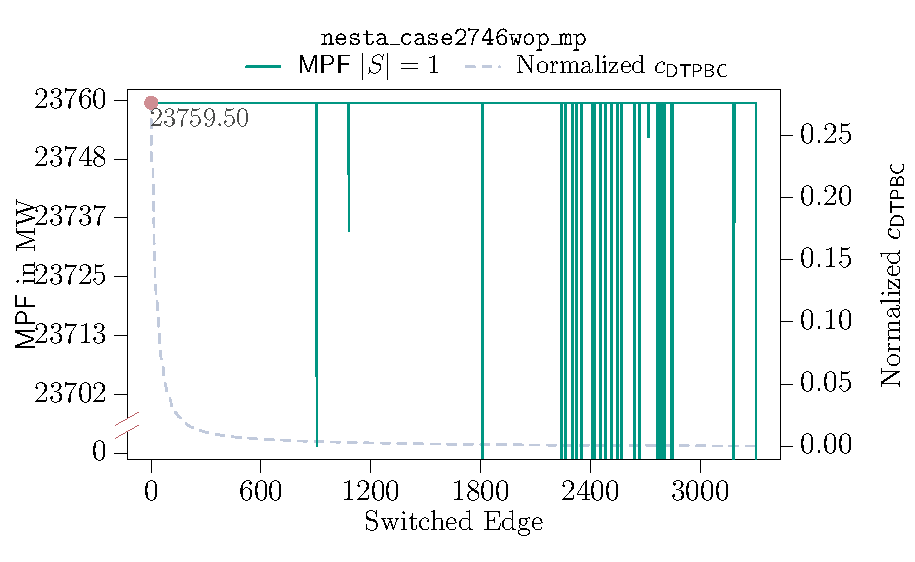
\includegraphics{switchplacement/plots/plot-SwitchingBetweenness_nesta_case2746wop_mp-dtpbc-mpf-cutY-StandAlone.pdf}%
            }%
            \label{ch:switching:sec:evaluation:plot:a:SwitchingBetweenness_nesta_case2746sp_mp_dtpbc_mpf_cutY}%
            \caption{}%
        \end{subfigure}%
        % 
    
        % 
        \hspace{-0.3cm}
        \begin{subfigure}[b]{.498\textwidth}%
            \centering%
            \resizebox {.865\columnwidth} {!} {
                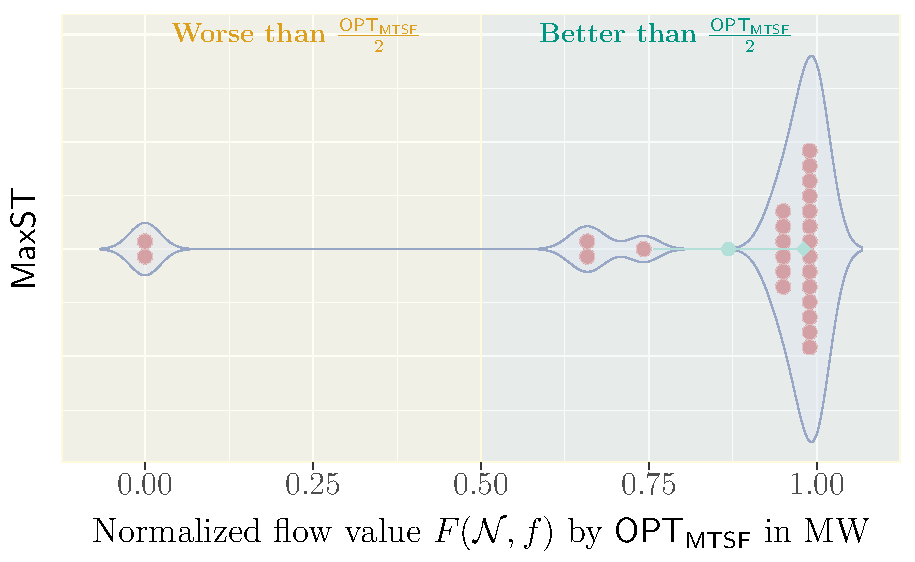
\includegraphics{switchplacement/plots/plot-maxst-vs-mtsf-violin-swarm-StandAlone.pdf}
                \label{ch:switching:sec:evaluation:plot:twoApproximation_violin}%
            }
            \caption{}%
        \end{subfigure}%
        % 
        \hfill%
        % 
        \begin{subfigure}[b]{.498\textwidth}%
            \centering%
            \resizebox {\columnwidth} {!} {
                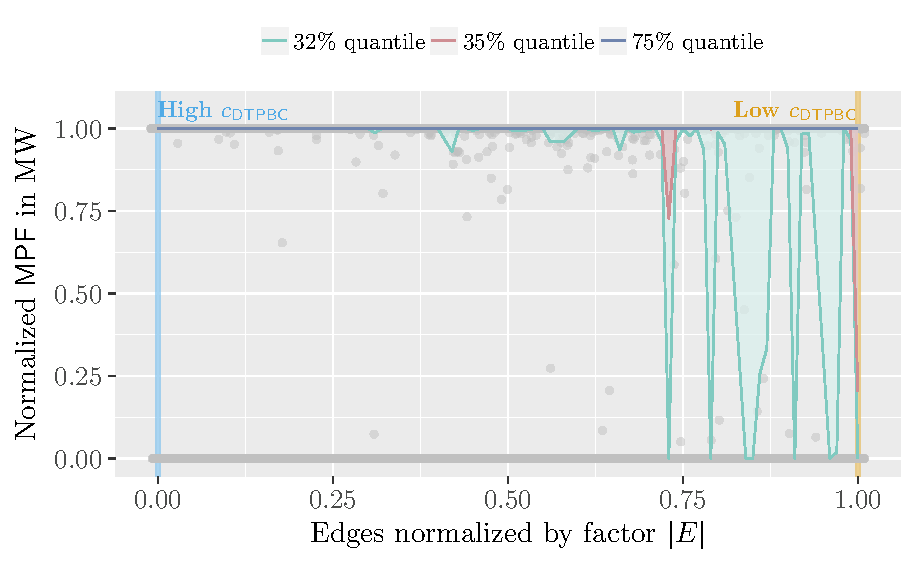
\includegraphics{switchplacement/plots/plot_dtp_betweenness_centrality_all_quantiles-StandAlone.pdf}
                % 
                \label{ch:switching:sec:evaluation:plot:dtp_betweenness_centrality_all_quantiles}%
            }%
            \caption{}%
            \label{ch:switching:sec:evaluation:fig:simulations:dtp}
        \end{subfigure}%
        % 
        %
        \caption[Simulation results for switching.]{Simulation evaluation using
        the data
        from~\cref{ch:switching:sec:evaluation:tbl:MTSF_MPF_PF_MF_long}~for~(c)
        and aggregating the results
        from~\crefrange{fig:Switching_Betweenness_Centrality_Plot_Cut_Y_3_to_24}
        {fig:Switching_Betweenness_Centrality_Plot_Cut_Y_162_to_3012} into (d)
        including (a) and (b). (a) and (b) show the
        \texttt{nesta\_case189\_edin} and \texttt{2746wop\_mp}, respectively,
        with the gray dashed line being the centrality of the edges (x-axis) and
        the green line the~\gls{mpf}~(y-axis). (c)~The~$2$-approximation on
        cacti using~\gls{maxst} is tested on arbitrary graphs. The global
        optimum~$\opt_{\gls{maxst}}$ is reached at~$1$ and the proven factor for
        cacti is at~$\nicefrac{1}{2}$. The green left (with range) and right
        point show the mean and median, respectively. (d)~The aggregated data
        are normalized with regards to the edges and~\gls{mpf}
        using~$\fmagnitude{\glssymbol{edges}}$ and the~\gls{mpf} of each of the
        network. The edges are ranked from highest to lowest~$c_{\sbc}$. The
        quantiles show that 32~\% of the test cases give worse results than the
        green line while switching an edge with low centrality.}%
        % 
        \label{ch:switching:sec:evaluation:fig:simulations}
    \end{figure}
\end{center}
\endgroup
% 
Recall that~$\opt_{\gls{mfp}}$ is an upper bound for~$\opt_{\gls{mtsfp}}$ and
that~\gls{mfp} and~\gls{mtsfp} are equal on trees. Thus,
from~\cref{ch:switching:sec:approximation_algorithm_on_cacti:lem:half_flow}
follows~\cref{ch:switching:sec:approximation_algorithm_on_cacti:thm:cacti_2_approximation}. %the next
% 
% 
%%%%%%%%%%%%%%%%%%%%%%%%%%%%%%%%%%%% THEOREM %%%%%%%%%%%%%%%%%%%%%%%%%%%%%%%%%%
\begin{theorem}
\label{ch:switching:sec:approximation_algorithm_on_cacti:thm:cacti_2_approximation}
% 
\cref{ch:switching:sec:approximation_algorithm_on_cacti:alg:factor_2_approximation}
is a factor~$2$-approximation algorithm for the~\gls{mfp} and~\gls{mtsfp} problem
on cacti.
\end{theorem}
% 
Note that an approximation ratio of~$\nicefrac{1}{2}$ does not provide a good
guarantee in the worst case. However, compared to other heuristics it gives
guarantees and can be used as an initial step for heuristics.
% 
% \clearpage
%%%%%%%%%%%%%%%%%%%%%%%%%%%%%%%%%%%%%%%%%%%%%%%%%%%%%%%%%%%%%%%%%%%%%%%%%%%%%%%
\section{Simulations}  
\label{ch:switching:sec:evaluation}
%%%%%%%%%%%%%%%%%%%%%%%%%%%%%%%%%%%%%%%%%%%%%%%%%%%%%%%%%%%%%%%%%%%%%%%%%%%%%%%
% 
We simulated\footnote{\href{https://i11www.iti.kit.edu/projects/mtsf/index}{https://i11www.iti.kit.edu/projects/mtsf/index}} 
% 
our~\gls{dtp}~betweenness centrality and 2-approximation algorithms for
penrose-minor-free graphs and cacti, respectively, on arbitrary graphs.
% 
By arbitrary graph we mean the~\gls{nesta} benchmark sets~\parencite{Cof14b},
which are based on the~\gls{ieee} benchmark
% 
sets~\parencite{online:IEEEtestData,Zimmerman2011a,4075418,Bil70,online:TheUniversityOfEdinburgh:SchoolOfMathematics:PowerSystemsTestCaseArchive,crow2015computational,Dem77,Gra03,780914,
Jos16,6120344,5589973,4113721,Woo13} and 
incorporate 
% 
realistic data such as thermal line limits. Note that we run our simulations on
arbitrary power grids, since there are not a lot of benchmark sets presenting
cacti namely \nestacase{3}, \texttt{4\_gs}, and~\texttt{9\_wscc} 
% 
% 
or~\source-\sink-networks available.
% 
%
Recall from~\cref{ch:switching:sec:model} that we have a disjoint set of
generators and consumers. This theoretical assumption cannot be found in any
benchmark set and realistic power grid. Thus, we have to modify the data in such
a way that we still provide a realistic benchmark set and comply with the
assumptions to avoid infinite generator production at buses having both
generators and consumers
(see~\cref{ch:switching:sec:model:eq:unlimited_generation_constraints,ch:switching:sec:model:eq:unlimited_demand_constraint}).
In addition, we only allow to consume a real power demand~$p_d$ at a real power
generator (see bus data's column three in the~\gls{ieee} Common Data
Format~\parencite{4075293}). All other consumers have an infinite maximum demand
(\cref{ch:switching:sec:model:eq:demand_constraint}). The results for the
problems in~\cref{ch:switching:sec:model} are shown
in~\cref{ch:switching:sec:evaluation:tbl:MTSF_MPF_PF_MF_long}.

For the 2-approximation, we use~\gls{maxst}
(\cref{ch:switching:sec:approximation_algorithm_on_cacti}) on different
benchmark data sets and compare the results with the~\gls{milp}
from~\cref{ch:switching:sec:model}. The algorithm~\gls{maxst} gives very good
results even though operating on arbitrary graphs
(see~\cref{ch:switching:sec:evaluation:tbl:MTSF_MPF_PF_MF_long}). Nearly
all---meaning~$93~\%$---of the results are better than the approximation factor
and~$82~\%$ are at most~$7~\%$ from the optimum value~$\opt_{\gls{mtsfp}}$
(see~\cref{ch:switching:sec:evaluation:fig:simulations}\screen{c}). Note
that~$36~\%$ of the results even reach the optimal value (cases equal
to~$\opt_{\gls{mtsfp}}$ have gray markers
in~\cref{ch:switching:sec:evaluation:tbl:MTSF_MPF_PF_MF_long}). Thus, the
expected quality on arbitrary graphs is much better than the proven
approximation ratio of~$2$ on cacti
(\cref{ch:switching:sec:approximation_algorithm_on_cacti}). There are two cases
worse than the approximation factor, because there is no feasible power flow for
the resulting networks~$\glssymbol{network}-\gls{switched}_{\gls{maxst}}$. There
are three cases in which the number of switched lines in the $2$-approximation
is greater than~$\opt_{\gls{mtsfp}}$. %Note that we do not optimize the number of
%switches.

The~\gls{dtp} is exact for~\source-\sink-penrose-minor-free graphs. There is no
benchmark case providing this structure. However, since the~\gls{dtp} represents
a distance measure, which marks interesting paths for switching, we introduced
the~\gls{dtp}-betweenness centrality
in~\cref{ch:switching:sec:exploit_structural_characteristics:def:dtp_betweenness_centrality}.
To estimate the relation of the power flow and the different edges having
different centrality values~$c_\sbc$ for the different benchmark cases with
different assorted characteristics, we calculated the~\gls{mpf} for the network
after removing a single edge~\edge with centrality~$c_\sbc(\edge)$ from the
network and decreasingly order the normalized edges by the centrality. Note that
we normalized the~\gls{mpf} and edge index by the network's~$\opt_{\gls{mpfp}}$
value and~$\fmagnitude{\gls{edges}}$, respectively. The normalization is
necessary to aggregate all cases
from~\crefrange{fig:Switching_Betweenness_Centrality_Plot_Cut_Y_3_to_24}
{fig:Switching_Betweenness_Centrality_Plot_Cut_Y_162_to_3012} into one plot.
The~$32~\%$ and~$35~\%$ quantiles
in~\cref{ch:switching:sec:evaluation:fig:simulations}\screen{d} show cut points
where the~\gls{mpf} decreases while switching an edge. These quantiles show
that~$32~\%$ of the test cases at low centrality result in worse results than
the plotted line. This effect happens mainly with edges having a small~$c_\sbc$
(\ie, the normalized edge index is close to~$1$). For the~$35~\%$ quantile there
are only deflections at edges with low centrality. Note, that the line at zero
represents~\nestacase{57}, \nestacase{2383}, and~\nestacase{3012}, where
switching of an edge leads to a network with no feasible~\gls{mpf}. Note that
deflection at edges with low centrality motivates the algorithm also
for~\gls{rop}, since edges with low centrality are more essential for the power
grid to get into a stable operation and should be considered first.
%
\begin{landscape}
    \begin{table}
        \centering
        \caption[Switching Results using the~\gls{nesta} Benchmark Sets.]{
        The~\gls{pf}, \gls{mpf}, \gls{mtsf} and~\gls{ots} models
        from~\cref{ch:switching:sec:model} are evaluated on the~\gls{nesta}
        benchmark sets~\parencite{Cof14b}. The
        parameters~$\fmagnitude{\glssymbol{vertices}}$, $
        \fmagnitude{\glssymbol{edges}}$, 
        and~$\fmagnitude{\glssymbol{switched}_{\glssymbol{problems}}}$ represent
        the number of vertices, edges and switched edges for a
        problem~$\glssymbol{problems}$, respectively, and the optimal solutions
        are given in~$\opt_{\glssymbol{problems}}$. Since~\gls{otsp}
        minimizes the cost, the flow value~$\flowvalue_{\gls{otsp}}$ is
        shown, too. The maximum possible generation is given in the last column
        (marked~\myhl{KITred15}{red} if it is larger than
        the~$\opt_{\gls{mfp}}$). The~\myhl{KITyellow15}{yellow} rows mark
        the interesting cases where~$\opt_{\gls{mpfp}}$ is smaller than
        the~$\opt_{\gls{mtsfp}}$. }
        %     
        %     
        %      However, the
        %     five cases in which the~$\opt_\mtsf$ is smaller than the~$\opt_\mf$ are
        %     marked~\myhl{KITblue15}{blue}. The cases in which the~$\opt_\maxst$
        %     (see~\cref{ch:switching:sec:approximation_algorithm_on_cacti})
        %     and~$\opt_\mpf$ are equal to~$\opt_\mtsf$ are
        %     marked~\myhl{KITblack!10}{gray}. In addition, there are three cases in
        %     which the number of switched lines in the~$\switched_\maxst$ is greater
        %     than in the~$\switched_\mtsf$ shown as~\myhl{KITgreen15}{green}. }
        % 
            \label{ch:switching:sec:evaluation:tbl:MTSF_MPF_PF_MF_long}
        % latex table generated in R 3.2.2 by xtable 1.8-0 package
% Fri Jan 26 22:50:42 2018
% \small
\footnotesize
\setlength{\tabcolsep}{4pt}
% \setlength\minrowclearance{3pt}
\begin{tabular}{lrrrrrrrrrrrrr}
  \toprule
  NESTA Case 
  &\hspace{-3mm} $\fmagnitude{\glssymbol{vertices}}$ 
  &\hspace{-3mm} $\fmagnitude{\glssymbol{edges}}$
  &\hspace{-3mm} $\fmagnitude{\glssymbol{switched}_{\gls{mtsfp}}}$ 
  &\hspace{-3mm} $\fmagnitude{\glssymbol{switched}_{\gls{otsp}}}$ 
  &\hspace{-3mm} $\fmagnitude{\glssymbol{switched}_{\gls{maxst}}}$ 
  &\hspace{-3mm} $\opt_{\gls{otsp}}$ in \$ 
  &\hspace{-3mm} $\flowvalue_{\gls{otsp}}$ 
  &\hspace{-3mm} $\opt_{\gls{pf}}$ 
  &\hspace{-3mm} $\opt_{\gls{mpfp}}$ 
  &\hspace{-3mm} $\opt_{\gls{mtsfp}}$ 
  &\hspace{-3mm} $\opt_{\gls{maxst}}$ 
  &\hspace{-3mm} $\opt_{\gls{mfp}}$ 
  &\hspace{-3mm} $\max$ Gen \\
 \midrule
\rowcolor{KITyellow15}\tablecase{nestacase3lmbd} &   3 &   3 & 1 & 1 & 1 &       5\,638.97 & 315 &      315.00 &      353.53 &  4\,000.00 & \cellcolor{KITblack!10} 4\,000.00 &  4\,000.00 &  4\,000.00 \\ 
  \tablecase{nestacase4gs} &   4 &   4 & \cellcolor{KITgreen15}0 & 1 & \cellcolor{KITgreen15}1 &           109.99 & 500 &      500.00 & \cellcolor{KITblack!10}     969.00 &      969.00 &      719.00 &      969.00 & \cellcolor{KITred15} 1\,639.00 \\ 
  \tablecase{nestacase5pjm} &   5 &   6 & \cellcolor{KITgreen15}0 & 1 & \cellcolor{KITgreen15}3 &      14\,991.30 & 1000 &  1\,000.00 & \cellcolor{KITblack!10} 1\,448.39 & \cellcolor{KITcyanblue15} 1\,448.39 &  1\,356.00 & \cellcolor{KITcyanblue15} 1\,530.00 &  1\,530.00 \\ 
  \tablecase{nestacase6c} &   6 &   7 & 4 & 1 & 4 &            22.77 & 107.5 &      107.50 & \cellcolor{KITblack!10}     370.00 &      370.00 &      248.00 &      370.00 & \cellcolor{KITred15} 1\,002.00 \\ 
  \rowcolor{KITyellow15}\tablecase{nestacase6ww} &   6 &  11 & 6 & 6 & 6 &       3\,046.41 & 210 &      210.00 &      332.80 & \cellcolor{KITcyanblue15}     360.00 & \cellcolor{KITblack!10}     360.00 & \cellcolor{KITcyanblue15}     470.00 & \cellcolor{KITred15}     530.00 \\ 
  \tablecase{nestacase9wscc} &   9 &   9 & 6 & 0 & 2 &       5\,216.03 & 315 &      315.00 & \cellcolor{KITblack!10}     770.00 &      770.00 & \cellcolor{KITblack!10}     770.00 &      770.00 & \cellcolor{KITred15}     820.00 \\ 
  \tablecase{nestacase14ieee} &  14 &  20 & 15 & 7 & 10 &           231.41 & 259 &      259.00 & \cellcolor{KITblack!10}     425.00 &      425.00 & \cellcolor{KITblack!10}     425.00 &      425.00 &      425.00 \\ 
  \tablecase{nestacase24ieeerts} &  24 &  38 & 28 & 10 & 18 &      61\,001.20 & 2850 &  2\,850.00 & \cellcolor{KITblack!10} 3\,405.00 &  3\,405.00 & \cellcolor{KITblack!10} 3\,405.00 &  3\,405.00 &  3\,405.00 \\ 
  \rowcolor{KITyellow15}\tablecase{nestacase29edin} &  29 &  99 & \cellcolor{KITgreen15}55 & 54 & \cellcolor{KITgreen15}79 &      29\,669.40 & 56325.9 & 56\,325.90 & 81\,597.50 & \cellcolor{KITcyanblue15}81\,603.40 & 76\,158.80 & \cellcolor{KITcyanblue15}82\,384.80 & 82\,384.80 \\ 
  \tablecase{nestacase30as} &  30 &  41 & 32 & 10 & 15 &           767.60 & 283.4 &      283.40 & \cellcolor{KITblack!10}     435.00 &      435.00 & \cellcolor{KITblack!10}     435.00 &      435.00 &      435.00 \\ 
  \tablecase{nestacase30fsr} &  30 &  41 & 30 & 14 & 15 &           565.21 & 189.2 &      189.20 & \cellcolor{KITblack!10}     335.00 &      335.00 &      322.20 &      335.00 &      335.00 \\ 
  \tablecase{nestacase30ieee} &  30 &  41 & 34 & 12 & 19 &           152.67 & 283.4 &      283.40 & \cellcolor{KITblack!10}     390.00 &      390.00 &      252.00 &      390.00 & \cellcolor{KITred15}     884.00 \\ 
  \tablecase{nestacase39epri} &  39 &  46 & 35 & 7 & 17 &      95\,578.30 & 6254.23 &  6\,254.23 & \cellcolor{KITblack!10} 7\,227.00 &  7\,227.00 & \cellcolor{KITblack!10} 7\,227.00 &  7\,227.00 & \cellcolor{KITred15} 7\,367.00 \\ 
  \tablecase{nestacase57ieee} &  57 &  80 & 75 & 25 & 40 &       1\,125.14 & 1250.8 &  1\,250.80 & \cellcolor{KITblack!10} 1\,377.00 &  1\,377.00 & \cellcolor{KITblack!10} 1\,377.00 &  1\,377.00 &  1\,377.00 \\ 
  \tablecase{nestacase73ieeerts} &  73 & 120 & 87 & 34 & 56 &     183\,004.00 & 8550 &  8\,550.00 & \cellcolor{KITblack!10}10\,215.00 & 10\,215.00 & \cellcolor{KITblack!10}10\,215.00 & 10\,215.00 & 10\,215.00 \\ 
  \tablecase{nestacase89pegase} &  89 & 210 & 145 & 70 & 142 &       5\,733.37 & 5733.37 &  5\,733.37 & \cellcolor{KITblack!10} 9\,921.23 &  9\,921.23 &  9\,718.23 &  9\,921.23 &  9\,921.23 \\ 
  \tablecase{nestacase118ieee} & 118 & 186 & 150 & --- & 92 & --- & --- &  4\,242.00 & \cellcolor{KITblack!10} 7\,119.00 & \cellcolor{KITcyanblue15} 7\,119.00 &  6\,830.00 & \cellcolor{KITcyanblue15} 7\,134.00 &  7\,134.00 \\ 
  \tablecase{nestacase162ieeedtc} & 162 & 284 & 269 & 77 & 154 &       3\,904.81 & 7239.06 &  7\,239.06 & \cellcolor{KITblack!10} 8\,296.00 &  8\,296.00 &  7\,931.00 &  8\,296.00 & \cellcolor{KITred15} 9\,685.00 \\ 
  \tablecase{nestacase189edin} & 189 & 206 & 71 & 62 & 62 &           783.95 & 1367.83 &  1\,367.83 & \cellcolor{KITblack!10} 2\,987.00 &  2\,987.00 & \cellcolor{KITblack!10} 2\,987.00 &  2\,987.00 & \cellcolor{KITred15} 3\,012.00 \\ 
  \tablecase{nestacase300ieee} & 300 & 411 & 290 & --- & 185 & --- & --- & 23\,527.20 & \cellcolor{KITblack!10}31\,568.00 & \cellcolor{KITcyanblue15}31\,568.00 & 30\,504.00 & \cellcolor{KITcyanblue15}31\,735.00 & \cellcolor{KITred15}32\,492.00 \\ 
  \tablecase{nestacase2736spmp} & 2736 & 3269 & 2518 & 545 & 1307 &     991\,228.00 & 18074.5 & 18\,074.50 & \cellcolor{KITblack!10}20\,246.70 & 20\,246.70 & 20\,010.70 & 20\,246.70 & 20\,246.70 \\ 
  \tablecase{nestacase2737sopmp} & 2737 & 3269 & 2536 & 630 & 1305 &     621\,780.00 & 11267.2 & 11\,267.20 & \cellcolor{KITblack!10}14\,677.90 & 14\,677.90 & 14\,537.20 & 14\,677.90 & 14\,677.90 \\ 
  \tablecase{nestacase2746wopmp} & 2746 & 3307 & 2547 & 649 & 1349 &     861\,568.00 & 18960 & 18\,960.00 & \cellcolor{KITblack!10}23\,759.50 & 23\,759.50 & --- & 23\,759.50 & 23\,759.50 \\ 
  \tablecase{nestacase2746wpmp} & 2746 & 3279 & 2487 & 594 & 1318 & 1\,261\,620.00 & 24873 & 24\,873.00 & \cellcolor{KITblack!10}27\,618.70 & 27\,618.70 & --- & 27\,618.70 & 27\,618.70 \\ 
  \tablecase{nestacase3120spmp} & 3120 & 3693 & 2793 & --- & 1513 & --- & --- & 21\,181.50 & \cellcolor{KITblack!10}25\,406.00 & 25\,406.00 & 24\,856.50 & 25\,406.00 & 25\,406.00 \\ 
   \bottomrule
\end{tabular}% table
    \end{table}
\end{landscape}
%
% 
%%%%%%%%%%%%%%%%%%%%%%%%%%%%%%%%%%%%%%%%%%%%%%%%%%%%%%%%%%%%%%%%%%%%%%%%%%%%%%%
%%%%%%%%%%%%%%%%%%%%%%%%%%%%%%%%%%%%%%%%%%%%%%%%%%%%%%%%%%%%%%%%%%%%%%%%%%%%%%%
\section{Conclusion}    
\label{ch:switching:sec:conclusion}
%%%%%%%%%%%%%%%%%%%%%%%%%%%%%%%%%%%%%%%%%%%%%%%%%%%%%%%%%%%%%%%%%%%%%%%%%%%%%%%
% 
This paper is the first to provide algorithms with provable guarantees
for~\gls{mtsfp} on certain graph structures and shrinks the gap between theory
and practice. In addition, it provides an extensive theoretical analysis of
the~\gls{mtsfp}, builds connections to related problems and shows how to
simplify the network including the transformations from a bounded to an 
unbounded~\gls{mtsfp}, and the equivalence of~\gls{otsp} and~\gls{mtsfp}. We
introduce an exact algorithm for networks with one generator and one consumer
for certain network structures and show when it becomes~\NP-hard
on~\source-\sink-networks. On that base, we define a new centrality measure
based on~\acrlong{dtp}{s} (\gls{dtp}{s}) representing
% 
the~\source-\sink-path with the smallest voltage angle difference. For multiple
generators and sinks in the network, we give a~$2$-approximation for cacti. At
the end, the complementing evaluation rounds off the theoretical results. The
simulations show very good results on the~\gls{nesta} benchmark set with
arbitrary graph structures, \ie, the results are in nearly all cases either
optimal or very close to the optimum.

However, there are many open problems. It is unknown if the reachability test
can be done in polynomial time and, if not, if there is still a polynomial time
algorithm for~\gls{dtp} (see discussion
in~\cref{ch:switching:sec:exploit_structural_characteristics:subsec:reachibility_test}).
Another open question is if there is a~\gls{ptas} on cacti. The current
idea is a rounding based algorithm. There are many other open problems such as
the complexity and the existence of algorithms while fixing a set of edges as
% 
non-switchable (motivated by~\gls{tnep}), as well as minimizing or
constraining the number of switches. In addition, we used a linearization of
the~\gls{ac}-model denoted by~\gls{dc}-model. Though, we could not
easily transfer our results directly to~\gls{ac}-power grids, the general
idea can be applied as a heuristic since it is based on the fact that the power
flow uses the path with the smallest resistance, which makes sense also with
the~\gls{ac}-model. However, the evaluation of that will be part of our
future research.
% 